\documentclass[t,xcolor=dvipsnames]{beamer}

%%%%%%%%%%%%%%%%%%%%%%%% Packages/includes
\usepackage[english]{babel}
%\usepackage[latin1]{inputenc}
\usepackage{times}
\usepackage{pgfpages}
\usepackage{pgfplotstable}
\usepackage{booktabs}
\usepackage{subcaption}
\usepackage{epigraph}
\usepackage{engord}
% Antonio's macros
% !TEX root = thesis.tex
\definecolor{accolornotes}{rgb}{0.7,0.3,0.2}
\newcommand{\acnote}[1]{\textcolor{accolornotes}{[{\bf #1}]}}


\definecolor{jscolornotes}{rgb}{0.3,0.7,0.2}
\newcommand{\jsnote}[1]{\textcolor{jscolornotes}{[{\bf #1}]}}


\definecolor{acgray}{rgb}{0.8,0.8,0.8}
\newcommand{\acremove}[1]{\textcolor{acgray}{[{#1}]}}

\definecolor{myred}{rgb}{0.6, 0, 0}
\definecolor{myblue}{rgb}{0.3, 0.1, 0.9}

%\definecolor{acgreen}{rgb}{0.1,0.5,0.1}
%\definecolor{acblue}{rgb}{0.1,0.1,0.5}
%\newcommand{\bl}[1]{\textcolor{acgreen}{#1}}
%\newcommand{\gr}[1]{\textcolor{acblue}{#1}}

\newcommand{\eg}{{\it e.g.}\ }
\newcommand{\ie}{{\it i.e.}\ }
\newcommand{\vs}{{vs.}\ }
\newcommand{\etal}{{et al.}\ }
%\newcommand{\cf}{{\it cf}}

\newcommand{\be}{\begin{equation}}
\newcommand{\ee}{\end{equation}}
\newcommand{\bea}{\begin{eqnarray}}
\newcommand{\eea}{\end{eqnarray}}
\newcommand{\beas}{\begin{eqnarray*}}
\newcommand{\eeas}{\end{eqnarray*}}

\usepackage{tikz}

\newcommand{\circleplus}{ 
  \mathbin{
    \mathchoice
      {\buildcircleplus{\displaystyle}}
      {\buildcircleplus{\textstyle}}
      {\buildcircleplus{\scriptstyle}}
      {\buildcircleplus{\scriptscriptstyle}}
  } 
}

\newcommand\buildcircleplus[1]{%
  \begin{tikzpicture}[baseline=(X.base), inner sep=0, outer sep=0]
    \node[draw,circle] (X)  {$#1+$};
  \end{tikzpicture}%
}


\newcommand{\reflabel}{dummy} % Dummy initial reflabel - use renewcommand at the start of each chapter

%%%
%%% Stuff for vector typesetting  ----------------------------------------
%%%
%%%    e.g. use "\v a" or "\v r" for vectors
%%%
\def\vec#1{\mathchoice{\mbox{\boldmath  $\displaystyle\bf#1$}}
{\mbox{\boldmath  $\textstyle\bf#1$}}
{\mbox{\boldmath  $\scriptstyle\bf#1$}}
{\mbox{\boldmath  $\scriptscriptstyle\bf#1$}}}
\def\v#1{\protect\vec #1}

%%%
%%% Stuff for matrix typesetting  ----------------------------------------
%%%
%%%    e.g. use "\m M" or "\m A" for matrices
%%%
\def\mat#1{\mathchoice{\mbox{\boldmath$\displaystyle\tt#1$}}
{\mbox{\boldmath$\textstyle\tt#1$}}
{\mbox{\boldmath$\scriptstyle\tt#1$}}
{\mbox{\boldmath$\scriptscriptstyle\tt#1$}}}
\def\m#1{\protect\mat #1}

%%%
%%% Stuff for bold maths typesetting  ----------------------------------------
%%%
%%%   e.g. use "\bfmu" for boldface mu symbol
%%%
\def\bfmu{\mbox{\boldmath$\mu$}}
\def\bftau{\mbox{\boldmath$\tau$}}
\def\bftheta{\mbox{\boldmath$\theta$}}
\def\bfdelta{\mbox{\boldmath$\delta$}}
\def\bfphi{\mbox{\boldmath$\phi$}}
\def\bfpsi{\mbox{\boldmath$\psi$}}
\def\bfeta{\mbox{\boldmath$\eta$}}
\def\bfnabla{\mbox{\boldmath$\nabla$}}
\def\bfGamma{\mbox{\boldmath$\Gamma$}}

%%%
%%% Stuff for argmax argmin  ----------------------------------------
%%%
\DeclareMathOperator*{\argmax}{argmax}
\DeclareMathOperator*{\argmin}{argmin}


%%%
%%% Stuff for calligraphic style  ----------------------------------------
%%%
\DeclareMathAlphabet{\mathcal}{OMS}{cmsy}{m}{n}

%% code to highlight maximal/minimal entries in column tables with pgftables
\newcommand{\findmax}[3]{
    \pgfplotstablevertcat{\datatable}{#1}
    \pgfplotstablecreatecol[
    create col/expr={%
    \pgfplotstablerow
    }]{rownumber}\datatable
    \pgfplotstablesort[sort key={#2},sort cmp={float >}]{\sorted}{\datatable}%
    \pgfplotstablegetelem{0}{rownumber}\of{\sorted}%
    \pgfmathtruncatemacro#3{\pgfplotsretval}
    \pgfplotstableclear{\datatable}
}

\newcommand{\findmin}[3]{
    \pgfplotstablevertcat{\datatable}{#1}
    \pgfplotstablecreatecol[
      create col/expr={%
    \pgfplotstablerow
    }]{rownumber}\datatable
    \pgfplotstablesort[sort key={#2},sort cmp={float <}]{\sorted}{\datatable}%
    \pgfplotstablegetelem{0}{rownumber}\of{\sorted}%
    \pgfmathtruncatemacro#3{\pgfplotsretval}
    \pgfplotstableclear{\datatable}
}

\pgfplotstableset{
    highlight col max/.code 2 args={
        \findmax{#1}{#2}{\maxval}
        \edef\setstyles{\noexpand\pgfplotstableset{
                every row \maxval\noexpand\space column #2/.style={
                    postproc cell content/.append style={
                        /pgfplots/table/@cell content/.add={$\noexpand\bf}{$}
                    },
                }
            }
        }\setstyles
    },
    highlight col min/.code 2 args={
        \findmin{#1}{#2}{\minval}
        \edef\setstyles{\noexpand\pgfplotstableset{
                every row \minval\noexpand\space column #2/.style={
                    postproc cell content/.append style={
                        /pgfplots/table/@cell content/.add={$\noexpand\bf}{$}
                    },
                }
            }
        }\setstyles
    },
    highlight row max/.code 2 args={
        \pgfmathtruncatemacro\rowindex{#2-1}
        \pgfplotstabletranspose{\transposed}{#1}
        \findmax{\transposed}{\rowindex}{\maxval}
        \edef\setstyles{\noexpand\pgfplotstableset{
                every row \rowindex\space column \maxval\noexpand/.style={
                    postproc cell content/.append style={
                        /pgfplots/table/@cell content/.add={$\noexpand\bf}{$}
                    },
                }
            }
        }\setstyles
    },
    highlight row min/.code 2 args={
        \pgfmathtruncatemacro\rowindex{#2-1}
        \pgfplotstabletranspose{\transposed}{#1}
        \findmin{\transposed}{\rowindex}{\maxval}
        \edef\setstyles{\noexpand\pgfplotstableset{
                every row \rowindex\space column \maxval\noexpand/.style={
                    postproc cell content/.append style={
                        /pgfplots/table/@cell content/.add={$\noexpand\bf}{$}
                    },
                }
            }
        }\setstyles
    },
}

\makeatletter
\long\def\pgfplotstabletypeset@opt@collectarg[#1]#2{%

    \pgfplotstable@isloadedtable{#2}%
        {\pgfplotstabletypeset@opt@[#1]{#2}}%
        {\pgfplotstabletypesetfile@opt@[#1]{#2}}%
}
\makeatother


\usepackage{tikz}
\usetikzlibrary{arrows,positioning,matrix,scopes,calc,tikzmark,decorations.pathreplacing,shapes,decorations.markings,calc}
\tikzstyle{every picture}+=[remember picture]

%%%%%%%%%%%%%%%%%%%%%%%% Bibliography
\usepackage[backend=bibtex,style=authortitle]{biblatex}
\AtEveryCitekey{\iffootnote{\color{black}\tiny}{\color{black}}}
\addbibresource{../references.bib}

%%%%%%%%%%%%%%%%%%%%%%%% Beamer Mode

%\setbeameroption{hide notes}
%\setbeameroption{show notes}
%\setbeameroption{show notes on second screen=right}


%%%%%%%%%%%%%%%%%%%%%%%% Beamer Options/Settings

\mode<presentation>
{
  \usetheme{default}
  \setbeamercovered{transparent}
}

\AtBeginSection[]{
  \usebackgroundtemplate{
  \tikz[overlay,remember picture] \node[opacity=0.2, at=(current page.center)] {
  \includegraphics[height=\paperheight,width=\paperwidth]{background}};
  }

  \begin{frame}
  \vfill
  \centering
  %\begin{beamercolorbox}[sep=8pt,center,shadow=true,rounded=true]{title}
    \usebeamerfont{title}\insertsectionhead\par%
  %\end{beamercolorbox}
  \vfill
  \end{frame}
  
  \usebackgroundtemplate{}
}

%\setbeamertemplate{note page}[plain]

% Get rid of the annoying symbol list
\beamertemplatenavigationsymbolsempty
% don't show bookmarks on initial view
\hypersetup{pdfpagemode=UseNone}

% Show page number in lower right
\setbeamertemplate{footline}{%
    \raisebox{5pt}{\makebox[\paperwidth]{\hfill\makebox[20pt]{\color{gray}
          \scriptsize\insertframenumber}}}\hspace*{5pt}}


\addtobeamertemplate{frametitle}{}{%
    \begin{tikzpicture}[remember picture,overlay]
    \node[anchor=north east,yshift=2pt] at (current page.north east) {
\includegraphics[height=1em]{uc-cmyk}};
    \end{tikzpicture}}

\definecolor{filtercolor}{RGB}{255,230,153}
\definecolor{filtershade}{RGB}{205,185,123}
\definecolor{fmcolor}{RGB}{231,230,230}
\definecolor{fmshade}{RGB}{186,185,185}

\setbeamercolor{title}{fg=White}
\setbeamercolor{author}{fg=White}
\setbeamercolor{institute}{fg=White}
\setbeamercolor{date}{fg=White}
%\setbeamercolor{section in head/foot}{fg=White}
%\setbeamercolor{author in head/foot}{fg=White}
%\setbeamercolor{date in head/foot}{fg=White}


%%%%%%%%%%%%%%%%%%%%%%%% Title Page Setup
\title[Structural Priors in Deep Networks] % (optional, use only with long paper titles)
{Structural Priors in Deep Networks}
%\subtitle
%{Improving CNN
%Generalization and
%Efficiency}

\author[Yani Ioannou]
{Yani Ioannou}

\institute[University of Cambridge] % (optional, but mostly needed)
{University of Cambridge}

\date{August 29, 2017}

%\pgfdeclareimage[height=0.5cm]{university-logo}{uc-cmyk}
%\logo{\pgfuseimage{university-logo}}

% Delete this, if you do not want the table of contents to pop up at
% the beginning of each subsection:
%\AtBeginSubsection[]
%{
%  \begin{frame}<beamer>{Outline}
%    \tableofcontents[currentsection,currentsubsection]
%  \end{frame}
%}

% If you wish to uncover everything in a step-wise fashion, uncomment
% the following command: 

%\beamerdefaultoverlayspecification{<+->}


\begin{document}

%%%%%%%%%%%%%%%%%%%% TITLE Frame

\usebackgroundtemplate{%             declare it
\tikz[overlay,remember picture] \node[opacity=0.95, at=(current page.center)] {
   \includegraphics[height=\paperheight,width=\paperwidth]{background}};
}

\begin{frame}
  \titlepage
\end{frame}


\usebackgroundtemplate{%             declare it
\tikz[overlay,remember picture] \node[opacity=0.2, at=(current page.center)] {
   \includegraphics[height=\paperheight,width=\paperwidth]{background}};
}

%\begin{frame}{Outline}
%  \tableofcontents
  % You might wish to add the option [pausesections]
%\end{frame}


% Since this a solution template for a generic talk, very little can
% be said about how it should be structured. However, the talk length
% of between 15min and 45min and the theme suggest that you stick to
% the following rules:  

\begin{frame}{Overview}
\tableofcontents
\end{frame}

% - Exactly two or three sections (other than the summary).
% - At *most* three subsections per section.
% - Talk about 30s to 2min per frame. So there should be between about
%   15 and 30 frames, all told.

\section{Introduction}

\begin{frame}{About Me}
\begin{itemize}
\item Ph.D.\ student in the Department of Engineering at the University of Cambridge.
\item Funded by a Microsoft Research PhD Scholarship
\item Supervised by Professor Roberto Cipolla, head of the Computer Vision and Robotics group in the Machine Intelligence Lab, and Dr. Antonio Criminisi, a principal researcher at Microsoft Research.
\end{itemize}
\centering
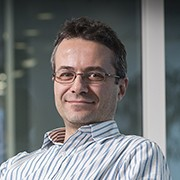
\includegraphics[width=0.207\linewidth]{antonio}~
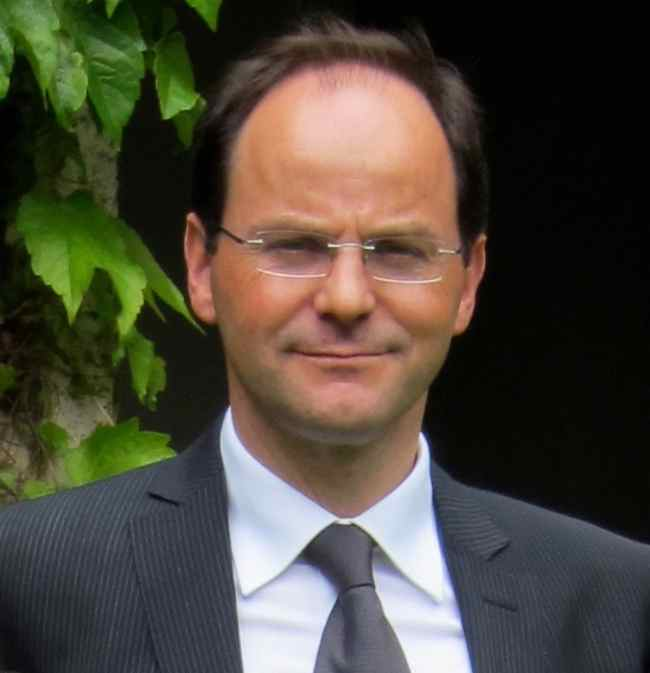
\includegraphics[width=0.2\linewidth]{roberto}
\end{frame}

\usebackgroundtemplate{}

\section{Research Overview}

\subsection{PhD Research}

\begin{frame}{First Author Publications during PhD}
\renewcommand{\thefootnote}{\fnsymbol{footnote}}
\begin{itemize}
    \item Decision Forests, Convolutional Networks and the Models in-Between.\\{\footnotesize Y.\ Ioannou, D.\ Robertson, D.\ Zikic, P.\ Kontschieder, J.\ Shotton, M.\ Brown, A.\ Criminisi.\\MSR Technical Report 2015} 
    \item \footnote{To be presented in this talk}Training CNNs with Low-Rank Filters for Efficient Image Classification.\\{\footnotesize Y.\ Ioannou, D.\ Robertson, J.\ Shotton, R.\ Cipolla, A.\ Criminisi. \\ICLR 2016}
    \item \footnotemark[1]Deep roots: Improving CNN efficiency with hierarchical filter groups.\\{\footnotesize Y.\ Ioannou, D.\ Robertson, R.\ Cipolla, A.\ Criminisi.\\CVPR 2017}
\end{itemize}
\end{frame}

\subsection{Collaborative Research}
\begin{frame}{Collaborative Research}
\begin{itemize}
    \item \textbf{Medical Computer Vision}
    \begin{itemize}
        \item Segmentation of brain tumor tissues with convolutional neural networks.\\{\footnotesize D.\ Zikic, Y.\ Ioannou, M.\ Brown, A.\ Criminisi. \textit{MICCAI-BRATS 2014}}
        \item Using CNNs for Malaria Diagnosis.\\{\footnotesize Intellectual Ventures/Gates Foundation}
    \end{itemize}
    \item \textbf{Adversarial Examples}\\Measuring Neural Net Robustness with Constraints.\\{\footnotesize O.\ Bastani, Y.\ Ioannou, L.\ Lampropoulos, D.\ Vytiniotis, A.\ Nori, A.\ Criminisi. \textit{NIPS 2016}}
    \item \textbf{Neural Network Design}\\Refining Architectures of Deep Convolutional Neural Networks.\\{\footnotesize 
S.\ Shankar, D.\ Robertson, Y.\ Ioannou, A.\ Criminisi, R.\ Cipolla. \textit{CVPR 2016}}
\end{itemize}
\end{frame}

\section{Motivation}

%%%%%%%%%%%%%%%%%%%%

\begin{frame}{ILSVRC}{Imagenet Large-Scale Visual Recognition Challenge}

\begin{figure}
    
\includegraphics[width=0.4\textwidth]{imagenetlogo}
\end{figure}
\begin{itemize}
    \item Imagenet Large-Scale Visual Recognition Challenge\footcite{ILSVRC2015}.
    \item 1.2 Million Training Images, 1000 classes.
    \item 50,000 image validiation/test set.
    \begin{itemize}
        \item In 2012 Alex Krizhevsky won challenge with CNN\footcite{Krizhevsky2012}.
        \item `AlexNet' was 26.2\% better than second best, 15.3\%.
    \end{itemize}
    \item State-of-the-art beats human error (5\%).
\end{itemize}    
\end{frame}


%%%%%%%%%%%%%%%%%%%%

\begin{frame}{AlexNet Complexity}
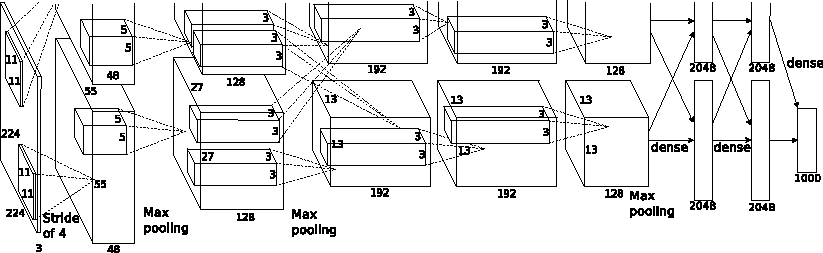
\includegraphics[width=\columnwidth]{alexnet}\footcite{Krizhevsky2012}
\begin{itemize}
\item $\approx$ 61 million parameters %60,965,224
\item $\approx$ 724 million FLOPS (per-sample) % 724,417,384
\item Imagenet has 1.28 million training samples ($227 \times 227 \times 3$) %227×227×3×1281167
\item Images of dimensions  ($227 \times 227 \times 3$) $\approx$ 200 billion pixels % %227×227×3×1281167 = 198,051,763,029
\end{itemize}
\end{frame}

\begin{frame}{AlexNet Complexity - FLOPS}
\centering
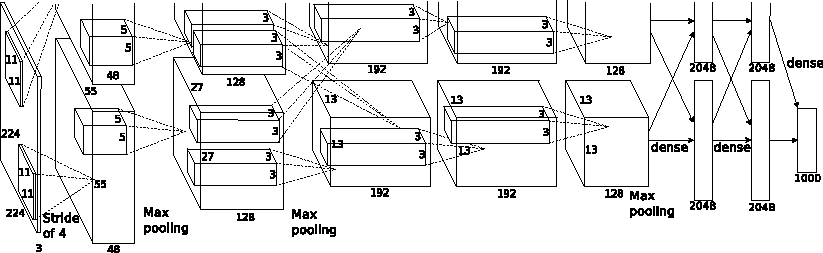
\includegraphics[width=0.9\columnwidth]{alexnet}
\tikzstyle{every node}=[font=\tiny]
\pgfplotstableread[col sep=comma]{alexnetma.csv}\datatable
\begin{tikzpicture}
\begin{axis}[
    axis x line=bottom,
    axis y line=left,
    ybar=0pt,
    bar width=1em,
    width=\linewidth,
    height=0.4\linewidth,
    enlarge x limits=0.1,
    ylabel=FLOPS,
    y label style={at={(axis description cs:0.09,.5)},anchor=south},
    y tick label style={
        /pgf/number format/.cd,
            fixed,
            fixed zerofill,
            precision=1,
        /tikz/.cd
    },
    ymin=0,
    xticklabels from table={\datatable}{layer},
    xticklabel style = {rotate = 90, xshift = -0.8ex, anchor = mid east, font=\tiny},
    xtick=data,
]
\addplot[ybar, draw=none, fill=red!40] table [x expr=\coordindex,y=ma]{\datatable};
\end{axis}
\end{tikzpicture}
\end{frame}

\begin{frame}{AlexNet Complexity - Parameters}
\centering
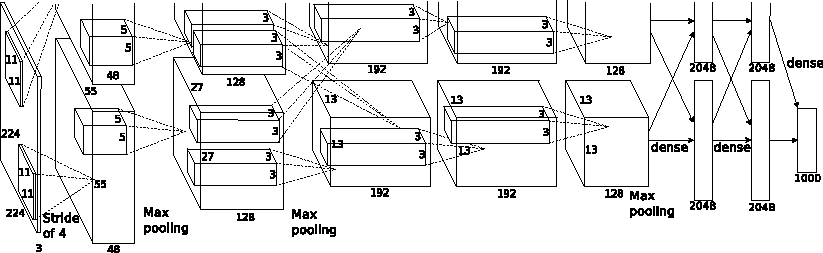
\includegraphics[width=0.9\columnwidth]{alexnet}
\tikzstyle{every node}=[font=\tiny]
\pgfplotstableread[col sep=comma]{alexnetma.csv}\datatable
\begin{tikzpicture}
\begin{axis}[
    axis x line=bottom,
    axis y line=left,
    ybar=0pt,
    bar width=1em,
    width=\linewidth,
    height=0.4\linewidth,
    enlarge x limits=0.1,
    ylabel=Parameters,
    y label style={at={(axis description cs:0.09,.5)},anchor=south},
    y tick label style={
        /pgf/number format/.cd,
            fixed,
            fixed zerofill,
            precision=1,
        /tikz/.cd
    },
    ymin=0,
    xticklabels from table={\datatable}{layer},
    xticklabel style = {rotate = 90, xshift = -0.8ex, anchor = mid east, font=\tiny},
    xtick=data,
]
\addplot[ybar, draw=none, fill=red!40] table [x expr=\coordindex,y=param]{\datatable};
\end{axis}
\end{tikzpicture}
$\approx$ 96\% in fully connected layers
%0.961714567
%0.038285433
\end{frame}

%%%%%%%%%%%%%%%%%%%%

\pgfplotstableread[col sep=comma]{../lrdata/bigpicture.csv}\datatable
\pgfplotstableread[col sep=comma]{../lrdata/bigpicture_ours.csv}\datatableours
\pgfplotstableread[col sep=comma]{../lrdata/bigpicture_aug.csv}\datatableaug
\pgfplotsset{major grid style={dotted,red}}
\pgfplotsset{minor grid style={dotted,red}}

\begin{frame}{}
\resizebox {\textwidth} {!} {
\begin{tikzpicture}
\begin{axis}[
  width=1.2\textwidth,
  height=1.3\textheight,
  axis x line=bottom,
  ylabel=Top-5 Error,
  xlabel=$\log_{10}$(Multiply-Accumulate Operations),
  axis lines=left,
%  enlarge x limits=0.05,
%  enlarge y limits=0.05,
  grid=both,
  ytick={0.00,0.02,...,0.22},
  xmode=log, 
  %ymin=0,ymax=0.2,
  xmin=10e7,xmax=10e13,
  yticklabel={\pgfmathparse{\tick*100}\pgfmathprintnumber{\pgfmathresult}\%},style={
        /pgf/number format/fixed,
        /pgf/number format/precision=1
  },
  legend style={at={(0.99,0.99)},anchor=north east},
]
%\addplot[mark=*,mark options={fill=green!70!black},nodes near coords,only marks,
%   point meta=explicit symbolic,
%   every node near coord/.append style={xshift=0.01em, anchor=west, font=\tiny},
%] table[meta=Network,x=Multiply-Acc.,y expr={1 - \thisrow{Top-5 Acc.} }]{\datatableours};
\addplot[mark=*,mark options={fill=blue},nodes near coords,only marks,
   point meta=explicit symbolic,
   every node near coord/.append style={xshift=0.01em, anchor=west, font=\tiny},
] table[meta=Network,x=Multiply-Acc.,y expr={1 - \thisrow{Top-5 Acc.} }]{\datatable};
\addplot[mark=square*,mark options={fill=red},nodes near coords,only marks,
   point meta=explicit symbolic,
   every node near coord/.append style={xshift=0.01em, anchor=west, font=\tiny},
] table[meta=Network,x=Test Multiply-Acc.,y expr={1 - \thisrow{Top-5 Acc.} }]{\datatableaug};
\legend{Crop \& Mirror Aug., Extra Augmentation}
\end{axis}
\end{tikzpicture}
}
\end{frame}

%%%%%%%%%%%%%%%%%%%%

\begin{frame}{}
\begin{figure}
\centering
\pgfplotstableread[col sep=comma]{../lrdata/bigpicture.csv}\datatable
\pgfplotstableread[col sep=comma]{../lrdata/bigpicture_ours.csv}\datatableours
\pgfplotstableread[col sep=comma]{../lrdata/bigpicture_aug.csv}\datatableaug
\pgfplotsset{major grid style={dotted,red}}
\pgfplotsset{minor grid style={dotted,red}}

\resizebox {\textwidth} {!} {
\begin{tikzpicture}
\begin{axis}[
  width=1.2\textwidth,
  height=1.1\textheight,
  axis x line=bottom,
  ylabel=Top-5 Error,
  xlabel=$\log_{10}$(Number of Parameters),
  axis lines=left,
  enlarge y limits=0.05,
  grid=both,
  ytick={0.01,0.02,...,0.2},
  xmode=log,
  xmin=10e6,xmax=10e8,
  yticklabel={\pgfmathparse{\tick*100}\pgfmathprintnumber{\pgfmathresult}\%},style={
        /pgf/number format/fixed,
        /pgf/number format/precision=1
  },
  legend style={at={(0.99,0.99)},anchor=north east},
]
%\addplot[mark=*,mark options={fill=green!70!black},
%   nodes near coords,
%   only marks,
%   point meta=explicit symbolic,
%   every node near coord/.append style={xshift=0.01em, anchor=west, font=\tiny},
%] table[meta=Network,x=Param.,y expr={1 - \thisrow{Top-5 Acc.} }]{\datatableours};
\addplot[mark=*,mark options={fill=blue},
   nodes near coords,
   only marks,
   point meta=explicit symbolic,
   every node near coord/.append style={xshift=0.01em, anchor=west, font=\tiny},
] table[meta=Network,x=Param.,y expr={1 - \thisrow{Top-5 Acc.} }]{\datatable};
\addplot[mark=square*,mark options={fill=red},
   nodes near coords,
   only marks,
   point meta=explicit symbolic,
   every node near coord/.append style={xshift=0.01em, anchor=west, font=\tiny},
   every node near coord/.append style={font=\tiny},
] table[meta=Network,x=Param.,y expr={1 - \thisrow{Top-5 Acc.} }]{\datatableaug};
\legend{Crop \& Mirror Aug., Extra Augmentation}
\end{axis}
\end{tikzpicture}
}
\end{figure}
\end{frame}

%%%%%%%%%%%%%%%%%%%%
\begin{frame}{The Problem}
% http://sms.cam.ac.uk/media/2017973?format=mpeg4&quality=720p
\begin{itemize}
%    \item Create a massively over-parameterized network, and ``regularize like hell'' to prevent over-fitting.
%    \item This seems to work well in practice for increasing generalization in networks such as VGG, and MSRA
    \item Creating a massively over-parameterized network, has consequences
    \item Training time: Translates into 2-3 weeks of training on 8 GPUs! (ResNet 200)
    \item Forward pass (ResNet 50): 12 ms GPU, 621 ms CPU
    \item Forward pass (GoogLeNet): 4.4 ms GPU, 300 ms CPU
\end{itemize}
\vfill
But what about the practicalities of using deep learning:
\begin{itemize}
    \item on embedded devices
    \item realtime applications
    \item backed by distributed/cloud computing
\end{itemize}
\end{frame}

\begin{frame}{Compression/Representation}
Isn't that already being addressed?
\begin{itemize}
\item Approximation (compression/pruning) of neural networks
\item Reduced representation (8-bit floats/binary!)
%\item Conditional computation
\end{itemize}
Allow us to have a trade off in compute \vs accuracy.
\vfill
\textit{These methods will still apply to any network.} Instead, let's try to  address the fundamental problem of over-parameterization.
\end{frame}
%%%%%%%%%%%%%%%%%%%%

\begin{frame}{Generalization and Num.\ Parameters}
	\begin{figure}[p]
		\centering
		\begin{subfigure}[t]{0.45\linewidth}
			\resizebox{\linewidth}{!}{%% Creator: Matplotlib, PGF backend
%%
%% To include the figure in your LaTeX document, write
%%   \input{<filename>.pgf}
%%
%% Make sure the required packages are loaded in your preamble
%%   \usepackage{pgf}
%%
%% Figures using additional raster images can only be included by \input if
%% they are in the same directory as the main LaTeX file. For loading figures
%% from other directories you can use the `import` package
%%   \usepackage{import}
%% and then include the figures with
%%   \import{<path to file>}{<filename>.pgf}
%%
%% Matplotlib used the following preamble
%%   \usepackage[utf8x]{inputenc}
%%   \usepackage[T1]{fontenc}
%%
\begingroup%
\makeatletter%
\begin{pgfpicture}%
\pgfpathrectangle{\pgfpointorigin}{\pgfqpoint{4.296389in}{2.655314in}}%
\pgfusepath{use as bounding box, clip}%
\begin{pgfscope}%
\pgfsetbuttcap%
\pgfsetmiterjoin%
\definecolor{currentfill}{rgb}{1.000000,1.000000,1.000000}%
\pgfsetfillcolor{currentfill}%
\pgfsetlinewidth{0.000000pt}%
\definecolor{currentstroke}{rgb}{1.000000,1.000000,1.000000}%
\pgfsetstrokecolor{currentstroke}%
\pgfsetdash{}{0pt}%
\pgfpathmoveto{\pgfqpoint{0.000000in}{0.000000in}}%
\pgfpathlineto{\pgfqpoint{4.296389in}{0.000000in}}%
\pgfpathlineto{\pgfqpoint{4.296389in}{2.655314in}}%
\pgfpathlineto{\pgfqpoint{0.000000in}{2.655314in}}%
\pgfpathclose%
\pgfusepath{fill}%
\end{pgfscope}%
\begin{pgfscope}%
\pgfsetbuttcap%
\pgfsetmiterjoin%
\definecolor{currentfill}{rgb}{1.000000,1.000000,1.000000}%
\pgfsetfillcolor{currentfill}%
\pgfsetlinewidth{0.000000pt}%
\definecolor{currentstroke}{rgb}{0.000000,0.000000,0.000000}%
\pgfsetstrokecolor{currentstroke}%
\pgfsetstrokeopacity{0.000000}%
\pgfsetdash{}{0pt}%
\pgfpathmoveto{\pgfqpoint{0.548317in}{0.386884in}}%
\pgfpathlineto{\pgfqpoint{4.124652in}{0.386884in}}%
\pgfpathlineto{\pgfqpoint{4.124652in}{2.488647in}}%
\pgfpathlineto{\pgfqpoint{0.548317in}{2.488647in}}%
\pgfpathclose%
\pgfusepath{fill}%
\end{pgfscope}%
\begin{pgfscope}%
\pgfsetbuttcap%
\pgfsetroundjoin%
\definecolor{currentfill}{rgb}{0.150000,0.150000,0.150000}%
\pgfsetfillcolor{currentfill}%
\pgfsetlinewidth{1.003750pt}%
\definecolor{currentstroke}{rgb}{0.150000,0.150000,0.150000}%
\pgfsetstrokecolor{currentstroke}%
\pgfsetdash{}{0pt}%
\pgfsys@defobject{currentmarker}{\pgfqpoint{0.000000in}{-0.083333in}}{\pgfqpoint{0.000000in}{0.000000in}}{%
\pgfpathmoveto{\pgfqpoint{0.000000in}{0.000000in}}%
\pgfpathlineto{\pgfqpoint{0.000000in}{-0.083333in}}%
\pgfusepath{stroke,fill}%
}%
\begin{pgfscope}%
\pgfsys@transformshift{0.548317in}{0.386884in}%
\pgfsys@useobject{currentmarker}{}%
\end{pgfscope}%
\end{pgfscope}%
\begin{pgfscope}%
\definecolor{textcolor}{rgb}{0.150000,0.150000,0.150000}%
\pgfsetstrokecolor{textcolor}%
\pgfsetfillcolor{textcolor}%
\pgftext[x=0.548317in,y=0.206329in,,top]{\color{textcolor}\sffamily\fontsize{10.000000}{12.000000}\selectfont \(\displaystyle 0.0\)}%
\end{pgfscope}%
\begin{pgfscope}%
\pgfsetbuttcap%
\pgfsetroundjoin%
\definecolor{currentfill}{rgb}{0.150000,0.150000,0.150000}%
\pgfsetfillcolor{currentfill}%
\pgfsetlinewidth{1.003750pt}%
\definecolor{currentstroke}{rgb}{0.150000,0.150000,0.150000}%
\pgfsetstrokecolor{currentstroke}%
\pgfsetdash{}{0pt}%
\pgfsys@defobject{currentmarker}{\pgfqpoint{0.000000in}{-0.083333in}}{\pgfqpoint{0.000000in}{0.000000in}}{%
\pgfpathmoveto{\pgfqpoint{0.000000in}{0.000000in}}%
\pgfpathlineto{\pgfqpoint{0.000000in}{-0.083333in}}%
\pgfusepath{stroke,fill}%
}%
\begin{pgfscope}%
\pgfsys@transformshift{1.263584in}{0.386884in}%
\pgfsys@useobject{currentmarker}{}%
\end{pgfscope}%
\end{pgfscope}%
\begin{pgfscope}%
\definecolor{textcolor}{rgb}{0.150000,0.150000,0.150000}%
\pgfsetstrokecolor{textcolor}%
\pgfsetfillcolor{textcolor}%
\pgftext[x=1.263584in,y=0.206329in,,top]{\color{textcolor}\sffamily\fontsize{10.000000}{12.000000}\selectfont \(\displaystyle 0.2\)}%
\end{pgfscope}%
\begin{pgfscope}%
\pgfsetbuttcap%
\pgfsetroundjoin%
\definecolor{currentfill}{rgb}{0.150000,0.150000,0.150000}%
\pgfsetfillcolor{currentfill}%
\pgfsetlinewidth{1.003750pt}%
\definecolor{currentstroke}{rgb}{0.150000,0.150000,0.150000}%
\pgfsetstrokecolor{currentstroke}%
\pgfsetdash{}{0pt}%
\pgfsys@defobject{currentmarker}{\pgfqpoint{0.000000in}{-0.083333in}}{\pgfqpoint{0.000000in}{0.000000in}}{%
\pgfpathmoveto{\pgfqpoint{0.000000in}{0.000000in}}%
\pgfpathlineto{\pgfqpoint{0.000000in}{-0.083333in}}%
\pgfusepath{stroke,fill}%
}%
\begin{pgfscope}%
\pgfsys@transformshift{1.978851in}{0.386884in}%
\pgfsys@useobject{currentmarker}{}%
\end{pgfscope}%
\end{pgfscope}%
\begin{pgfscope}%
\definecolor{textcolor}{rgb}{0.150000,0.150000,0.150000}%
\pgfsetstrokecolor{textcolor}%
\pgfsetfillcolor{textcolor}%
\pgftext[x=1.978851in,y=0.206329in,,top]{\color{textcolor}\sffamily\fontsize{10.000000}{12.000000}\selectfont \(\displaystyle 0.4\)}%
\end{pgfscope}%
\begin{pgfscope}%
\pgfsetbuttcap%
\pgfsetroundjoin%
\definecolor{currentfill}{rgb}{0.150000,0.150000,0.150000}%
\pgfsetfillcolor{currentfill}%
\pgfsetlinewidth{1.003750pt}%
\definecolor{currentstroke}{rgb}{0.150000,0.150000,0.150000}%
\pgfsetstrokecolor{currentstroke}%
\pgfsetdash{}{0pt}%
\pgfsys@defobject{currentmarker}{\pgfqpoint{0.000000in}{-0.083333in}}{\pgfqpoint{0.000000in}{0.000000in}}{%
\pgfpathmoveto{\pgfqpoint{0.000000in}{0.000000in}}%
\pgfpathlineto{\pgfqpoint{0.000000in}{-0.083333in}}%
\pgfusepath{stroke,fill}%
}%
\begin{pgfscope}%
\pgfsys@transformshift{2.694118in}{0.386884in}%
\pgfsys@useobject{currentmarker}{}%
\end{pgfscope}%
\end{pgfscope}%
\begin{pgfscope}%
\definecolor{textcolor}{rgb}{0.150000,0.150000,0.150000}%
\pgfsetstrokecolor{textcolor}%
\pgfsetfillcolor{textcolor}%
\pgftext[x=2.694118in,y=0.206329in,,top]{\color{textcolor}\sffamily\fontsize{10.000000}{12.000000}\selectfont \(\displaystyle 0.6\)}%
\end{pgfscope}%
\begin{pgfscope}%
\pgfsetbuttcap%
\pgfsetroundjoin%
\definecolor{currentfill}{rgb}{0.150000,0.150000,0.150000}%
\pgfsetfillcolor{currentfill}%
\pgfsetlinewidth{1.003750pt}%
\definecolor{currentstroke}{rgb}{0.150000,0.150000,0.150000}%
\pgfsetstrokecolor{currentstroke}%
\pgfsetdash{}{0pt}%
\pgfsys@defobject{currentmarker}{\pgfqpoint{0.000000in}{-0.083333in}}{\pgfqpoint{0.000000in}{0.000000in}}{%
\pgfpathmoveto{\pgfqpoint{0.000000in}{0.000000in}}%
\pgfpathlineto{\pgfqpoint{0.000000in}{-0.083333in}}%
\pgfusepath{stroke,fill}%
}%
\begin{pgfscope}%
\pgfsys@transformshift{3.409385in}{0.386884in}%
\pgfsys@useobject{currentmarker}{}%
\end{pgfscope}%
\end{pgfscope}%
\begin{pgfscope}%
\definecolor{textcolor}{rgb}{0.150000,0.150000,0.150000}%
\pgfsetstrokecolor{textcolor}%
\pgfsetfillcolor{textcolor}%
\pgftext[x=3.409385in,y=0.206329in,,top]{\color{textcolor}\sffamily\fontsize{10.000000}{12.000000}\selectfont \(\displaystyle 0.8\)}%
\end{pgfscope}%
\begin{pgfscope}%
\pgfsetbuttcap%
\pgfsetroundjoin%
\definecolor{currentfill}{rgb}{0.150000,0.150000,0.150000}%
\pgfsetfillcolor{currentfill}%
\pgfsetlinewidth{1.003750pt}%
\definecolor{currentstroke}{rgb}{0.150000,0.150000,0.150000}%
\pgfsetstrokecolor{currentstroke}%
\pgfsetdash{}{0pt}%
\pgfsys@defobject{currentmarker}{\pgfqpoint{0.000000in}{-0.083333in}}{\pgfqpoint{0.000000in}{0.000000in}}{%
\pgfpathmoveto{\pgfqpoint{0.000000in}{0.000000in}}%
\pgfpathlineto{\pgfqpoint{0.000000in}{-0.083333in}}%
\pgfusepath{stroke,fill}%
}%
\begin{pgfscope}%
\pgfsys@transformshift{4.124652in}{0.386884in}%
\pgfsys@useobject{currentmarker}{}%
\end{pgfscope}%
\end{pgfscope}%
\begin{pgfscope}%
\definecolor{textcolor}{rgb}{0.150000,0.150000,0.150000}%
\pgfsetstrokecolor{textcolor}%
\pgfsetfillcolor{textcolor}%
\pgftext[x=4.124652in,y=0.206329in,,top]{\color{textcolor}\sffamily\fontsize{10.000000}{12.000000}\selectfont \(\displaystyle 1.0\)}%
\end{pgfscope}%
\begin{pgfscope}%
\pgfsetbuttcap%
\pgfsetroundjoin%
\definecolor{currentfill}{rgb}{0.150000,0.150000,0.150000}%
\pgfsetfillcolor{currentfill}%
\pgfsetlinewidth{1.003750pt}%
\definecolor{currentstroke}{rgb}{0.150000,0.150000,0.150000}%
\pgfsetstrokecolor{currentstroke}%
\pgfsetdash{}{0pt}%
\pgfsys@defobject{currentmarker}{\pgfqpoint{-0.083333in}{0.000000in}}{\pgfqpoint{0.000000in}{0.000000in}}{%
\pgfpathmoveto{\pgfqpoint{0.000000in}{0.000000in}}%
\pgfpathlineto{\pgfqpoint{-0.083333in}{0.000000in}}%
\pgfusepath{stroke,fill}%
}%
\begin{pgfscope}%
\pgfsys@transformshift{0.548317in}{0.386884in}%
\pgfsys@useobject{currentmarker}{}%
\end{pgfscope}%
\end{pgfscope}%
\begin{pgfscope}%
\definecolor{textcolor}{rgb}{0.150000,0.150000,0.150000}%
\pgfsetstrokecolor{textcolor}%
\pgfsetfillcolor{textcolor}%
\pgftext[x=0.082267in,y=0.336742in,left,base]{\color{textcolor}\sffamily\fontsize{10.000000}{12.000000}\selectfont \(\displaystyle -1.0\)}%
\end{pgfscope}%
\begin{pgfscope}%
\pgfsetbuttcap%
\pgfsetroundjoin%
\definecolor{currentfill}{rgb}{0.150000,0.150000,0.150000}%
\pgfsetfillcolor{currentfill}%
\pgfsetlinewidth{1.003750pt}%
\definecolor{currentstroke}{rgb}{0.150000,0.150000,0.150000}%
\pgfsetstrokecolor{currentstroke}%
\pgfsetdash{}{0pt}%
\pgfsys@defobject{currentmarker}{\pgfqpoint{-0.083333in}{0.000000in}}{\pgfqpoint{0.000000in}{0.000000in}}{%
\pgfpathmoveto{\pgfqpoint{0.000000in}{0.000000in}}%
\pgfpathlineto{\pgfqpoint{-0.083333in}{0.000000in}}%
\pgfusepath{stroke,fill}%
}%
\begin{pgfscope}%
\pgfsys@transformshift{0.548317in}{0.912325in}%
\pgfsys@useobject{currentmarker}{}%
\end{pgfscope}%
\end{pgfscope}%
\begin{pgfscope}%
\definecolor{textcolor}{rgb}{0.150000,0.150000,0.150000}%
\pgfsetstrokecolor{textcolor}%
\pgfsetfillcolor{textcolor}%
\pgftext[x=0.082267in,y=0.862183in,left,base]{\color{textcolor}\sffamily\fontsize{10.000000}{12.000000}\selectfont \(\displaystyle -0.5\)}%
\end{pgfscope}%
\begin{pgfscope}%
\pgfsetbuttcap%
\pgfsetroundjoin%
\definecolor{currentfill}{rgb}{0.150000,0.150000,0.150000}%
\pgfsetfillcolor{currentfill}%
\pgfsetlinewidth{1.003750pt}%
\definecolor{currentstroke}{rgb}{0.150000,0.150000,0.150000}%
\pgfsetstrokecolor{currentstroke}%
\pgfsetdash{}{0pt}%
\pgfsys@defobject{currentmarker}{\pgfqpoint{-0.083333in}{0.000000in}}{\pgfqpoint{0.000000in}{0.000000in}}{%
\pgfpathmoveto{\pgfqpoint{0.000000in}{0.000000in}}%
\pgfpathlineto{\pgfqpoint{-0.083333in}{0.000000in}}%
\pgfusepath{stroke,fill}%
}%
\begin{pgfscope}%
\pgfsys@transformshift{0.548317in}{1.437766in}%
\pgfsys@useobject{currentmarker}{}%
\end{pgfscope}%
\end{pgfscope}%
\begin{pgfscope}%
\definecolor{textcolor}{rgb}{0.150000,0.150000,0.150000}%
\pgfsetstrokecolor{textcolor}%
\pgfsetfillcolor{textcolor}%
\pgftext[x=0.190292in,y=1.387624in,left,base]{\color{textcolor}\sffamily\fontsize{10.000000}{12.000000}\selectfont \(\displaystyle 0.0\)}%
\end{pgfscope}%
\begin{pgfscope}%
\pgfsetbuttcap%
\pgfsetroundjoin%
\definecolor{currentfill}{rgb}{0.150000,0.150000,0.150000}%
\pgfsetfillcolor{currentfill}%
\pgfsetlinewidth{1.003750pt}%
\definecolor{currentstroke}{rgb}{0.150000,0.150000,0.150000}%
\pgfsetstrokecolor{currentstroke}%
\pgfsetdash{}{0pt}%
\pgfsys@defobject{currentmarker}{\pgfqpoint{-0.083333in}{0.000000in}}{\pgfqpoint{0.000000in}{0.000000in}}{%
\pgfpathmoveto{\pgfqpoint{0.000000in}{0.000000in}}%
\pgfpathlineto{\pgfqpoint{-0.083333in}{0.000000in}}%
\pgfusepath{stroke,fill}%
}%
\begin{pgfscope}%
\pgfsys@transformshift{0.548317in}{1.963207in}%
\pgfsys@useobject{currentmarker}{}%
\end{pgfscope}%
\end{pgfscope}%
\begin{pgfscope}%
\definecolor{textcolor}{rgb}{0.150000,0.150000,0.150000}%
\pgfsetstrokecolor{textcolor}%
\pgfsetfillcolor{textcolor}%
\pgftext[x=0.190292in,y=1.913065in,left,base]{\color{textcolor}\sffamily\fontsize{10.000000}{12.000000}\selectfont \(\displaystyle 0.5\)}%
\end{pgfscope}%
\begin{pgfscope}%
\pgfsetbuttcap%
\pgfsetroundjoin%
\definecolor{currentfill}{rgb}{0.150000,0.150000,0.150000}%
\pgfsetfillcolor{currentfill}%
\pgfsetlinewidth{1.003750pt}%
\definecolor{currentstroke}{rgb}{0.150000,0.150000,0.150000}%
\pgfsetstrokecolor{currentstroke}%
\pgfsetdash{}{0pt}%
\pgfsys@defobject{currentmarker}{\pgfqpoint{-0.083333in}{0.000000in}}{\pgfqpoint{0.000000in}{0.000000in}}{%
\pgfpathmoveto{\pgfqpoint{0.000000in}{0.000000in}}%
\pgfpathlineto{\pgfqpoint{-0.083333in}{0.000000in}}%
\pgfusepath{stroke,fill}%
}%
\begin{pgfscope}%
\pgfsys@transformshift{0.548317in}{2.488647in}%
\pgfsys@useobject{currentmarker}{}%
\end{pgfscope}%
\end{pgfscope}%
\begin{pgfscope}%
\definecolor{textcolor}{rgb}{0.150000,0.150000,0.150000}%
\pgfsetstrokecolor{textcolor}%
\pgfsetfillcolor{textcolor}%
\pgftext[x=0.190292in,y=2.438505in,left,base]{\color{textcolor}\sffamily\fontsize{10.000000}{12.000000}\selectfont \(\displaystyle 1.0\)}%
\end{pgfscope}%
\begin{pgfscope}%
\pgfpathrectangle{\pgfqpoint{0.548317in}{0.386884in}}{\pgfqpoint{3.576335in}{2.101763in}} %
\pgfusepath{clip}%
\pgfsetbuttcap%
\pgfsetroundjoin%
\definecolor{currentfill}{rgb}{0.400000,0.760784,0.647059}%
\pgfsetfillcolor{currentfill}%
\pgfsetlinewidth{0.000000pt}%
\definecolor{currentstroke}{rgb}{0.400000,0.760784,0.647059}%
\pgfsetstrokecolor{currentstroke}%
\pgfsetdash{}{0pt}%
\pgfsys@defobject{currentmarker}{\pgfqpoint{-0.048611in}{-0.048611in}}{\pgfqpoint{0.048611in}{0.048611in}}{%
\pgfpathmoveto{\pgfqpoint{0.000000in}{-0.048611in}}%
\pgfpathcurveto{\pgfqpoint{0.012892in}{-0.048611in}}{\pgfqpoint{0.025257in}{-0.043489in}}{\pgfqpoint{0.034373in}{-0.034373in}}%
\pgfpathcurveto{\pgfqpoint{0.043489in}{-0.025257in}}{\pgfqpoint{0.048611in}{-0.012892in}}{\pgfqpoint{0.048611in}{0.000000in}}%
\pgfpathcurveto{\pgfqpoint{0.048611in}{0.012892in}}{\pgfqpoint{0.043489in}{0.025257in}}{\pgfqpoint{0.034373in}{0.034373in}}%
\pgfpathcurveto{\pgfqpoint{0.025257in}{0.043489in}}{\pgfqpoint{0.012892in}{0.048611in}}{\pgfqpoint{0.000000in}{0.048611in}}%
\pgfpathcurveto{\pgfqpoint{-0.012892in}{0.048611in}}{\pgfqpoint{-0.025257in}{0.043489in}}{\pgfqpoint{-0.034373in}{0.034373in}}%
\pgfpathcurveto{\pgfqpoint{-0.043489in}{0.025257in}}{\pgfqpoint{-0.048611in}{0.012892in}}{\pgfqpoint{-0.048611in}{0.000000in}}%
\pgfpathcurveto{\pgfqpoint{-0.048611in}{-0.012892in}}{\pgfqpoint{-0.043489in}{-0.025257in}}{\pgfqpoint{-0.034373in}{-0.034373in}}%
\pgfpathcurveto{\pgfqpoint{-0.025257in}{-0.043489in}}{\pgfqpoint{-0.012892in}{-0.048611in}}{\pgfqpoint{0.000000in}{-0.048611in}}%
\pgfpathclose%
\pgfusepath{fill}%
}%
\begin{pgfscope}%
\pgfsys@transformshift{2.260811in}{0.754316in}%
\pgfsys@useobject{currentmarker}{}%
\end{pgfscope}%
\begin{pgfscope}%
\pgfsys@transformshift{2.611975in}{0.899184in}%
\pgfsys@useobject{currentmarker}{}%
\end{pgfscope}%
\begin{pgfscope}%
\pgfsys@transformshift{3.012052in}{1.144101in}%
\pgfsys@useobject{currentmarker}{}%
\end{pgfscope}%
\end{pgfscope}%
\begin{pgfscope}%
\pgfpathrectangle{\pgfqpoint{0.548317in}{0.386884in}}{\pgfqpoint{3.576335in}{2.101763in}} %
\pgfusepath{clip}%
\pgfsetbuttcap%
\pgfsetroundjoin%
\pgfsetlinewidth{1.756562pt}%
\definecolor{currentstroke}{rgb}{0.988235,0.552941,0.384314}%
\pgfsetstrokecolor{currentstroke}%
\pgfsetdash{{5.600000pt}{2.400000pt}}{0.000000pt}%
\pgfpathmoveto{\pgfqpoint{0.534428in}{0.382588in}}%
\pgfpathlineto{\pgfqpoint{0.584442in}{0.397288in}}%
\pgfpathlineto{\pgfqpoint{0.656691in}{0.416887in}}%
\pgfpathlineto{\pgfqpoint{0.728940in}{0.435004in}}%
\pgfpathlineto{\pgfqpoint{0.801189in}{0.451796in}}%
\pgfpathlineto{\pgfqpoint{0.873438in}{0.467418in}}%
\pgfpathlineto{\pgfqpoint{0.945688in}{0.482026in}}%
\pgfpathlineto{\pgfqpoint{1.017937in}{0.495776in}}%
\pgfpathlineto{\pgfqpoint{1.090186in}{0.508825in}}%
\pgfpathlineto{\pgfqpoint{1.162435in}{0.521328in}}%
\pgfpathlineto{\pgfqpoint{1.234684in}{0.533440in}}%
\pgfpathlineto{\pgfqpoint{1.306933in}{0.545319in}}%
\pgfpathlineto{\pgfqpoint{1.379183in}{0.557120in}}%
\pgfpathlineto{\pgfqpoint{1.451432in}{0.568999in}}%
\pgfpathlineto{\pgfqpoint{1.523681in}{0.581112in}}%
\pgfpathlineto{\pgfqpoint{1.595930in}{0.593615in}}%
\pgfpathlineto{\pgfqpoint{1.668179in}{0.606663in}}%
\pgfpathlineto{\pgfqpoint{1.740429in}{0.620414in}}%
\pgfpathlineto{\pgfqpoint{1.812678in}{0.635022in}}%
\pgfpathlineto{\pgfqpoint{1.884927in}{0.650644in}}%
\pgfpathlineto{\pgfqpoint{1.957176in}{0.667435in}}%
\pgfpathlineto{\pgfqpoint{2.029425in}{0.685553in}}%
\pgfpathlineto{\pgfqpoint{2.101675in}{0.705151in}}%
\pgfpathlineto{\pgfqpoint{2.173924in}{0.726388in}}%
\pgfpathlineto{\pgfqpoint{2.246173in}{0.749418in}}%
\pgfpathlineto{\pgfqpoint{2.318422in}{0.774397in}}%
\pgfpathlineto{\pgfqpoint{2.390671in}{0.801482in}}%
\pgfpathlineto{\pgfqpoint{2.462921in}{0.830828in}}%
\pgfpathlineto{\pgfqpoint{2.535170in}{0.862592in}}%
\pgfpathlineto{\pgfqpoint{2.607419in}{0.896929in}}%
\pgfpathlineto{\pgfqpoint{2.679668in}{0.933995in}}%
\pgfpathlineto{\pgfqpoint{2.751917in}{0.973947in}}%
\pgfpathlineto{\pgfqpoint{2.824166in}{1.016940in}}%
\pgfpathlineto{\pgfqpoint{2.896416in}{1.063129in}}%
\pgfpathlineto{\pgfqpoint{2.968665in}{1.112672in}}%
\pgfpathlineto{\pgfqpoint{3.040914in}{1.165725in}}%
\pgfpathlineto{\pgfqpoint{3.113163in}{1.222442in}}%
\pgfpathlineto{\pgfqpoint{3.185412in}{1.282980in}}%
\pgfpathlineto{\pgfqpoint{3.257662in}{1.347495in}}%
\pgfpathlineto{\pgfqpoint{3.329911in}{1.416143in}}%
\pgfpathlineto{\pgfqpoint{3.402160in}{1.489080in}}%
\pgfpathlineto{\pgfqpoint{3.474409in}{1.566461in}}%
\pgfpathlineto{\pgfqpoint{3.546658in}{1.648444in}}%
\pgfpathlineto{\pgfqpoint{3.618908in}{1.735183in}}%
\pgfpathlineto{\pgfqpoint{3.691157in}{1.826835in}}%
\pgfpathlineto{\pgfqpoint{3.763406in}{1.923556in}}%
\pgfpathlineto{\pgfqpoint{3.835655in}{2.025501in}}%
\pgfpathlineto{\pgfqpoint{3.907904in}{2.132827in}}%
\pgfpathlineto{\pgfqpoint{3.980154in}{2.245689in}}%
\pgfpathlineto{\pgfqpoint{4.052403in}{2.364244in}}%
\pgfpathlineto{\pgfqpoint{4.124652in}{2.488647in}}%
\pgfusepath{stroke}%
\end{pgfscope}%
\begin{pgfscope}%
\pgfpathrectangle{\pgfqpoint{0.548317in}{0.386884in}}{\pgfqpoint{3.576335in}{2.101763in}} %
\pgfusepath{clip}%
\pgfsetroundcap%
\pgfsetroundjoin%
\pgfsetlinewidth{1.756562pt}%
\definecolor{currentstroke}{rgb}{0.552941,0.627451,0.796078}%
\pgfsetstrokecolor{currentstroke}%
\pgfsetdash{}{0pt}%
\pgfpathmoveto{\pgfqpoint{0.534428in}{0.664235in}}%
\pgfpathlineto{\pgfqpoint{0.584442in}{0.658600in}}%
\pgfpathlineto{\pgfqpoint{0.656691in}{0.650850in}}%
\pgfpathlineto{\pgfqpoint{0.728940in}{0.643574in}}%
\pgfpathlineto{\pgfqpoint{0.801189in}{0.636856in}}%
\pgfpathlineto{\pgfqpoint{0.873438in}{0.630780in}}%
\pgfpathlineto{\pgfqpoint{0.945688in}{0.625432in}}%
\pgfpathlineto{\pgfqpoint{1.017937in}{0.620894in}}%
\pgfpathlineto{\pgfqpoint{1.090186in}{0.617252in}}%
\pgfpathlineto{\pgfqpoint{1.162435in}{0.614590in}}%
\pgfpathlineto{\pgfqpoint{1.234684in}{0.612992in}}%
\pgfpathlineto{\pgfqpoint{1.306933in}{0.612542in}}%
\pgfpathlineto{\pgfqpoint{1.379183in}{0.613325in}}%
\pgfpathlineto{\pgfqpoint{1.451432in}{0.615424in}}%
\pgfpathlineto{\pgfqpoint{1.523681in}{0.618925in}}%
\pgfpathlineto{\pgfqpoint{1.595930in}{0.623912in}}%
\pgfpathlineto{\pgfqpoint{1.668179in}{0.630468in}}%
\pgfpathlineto{\pgfqpoint{1.740429in}{0.638678in}}%
\pgfpathlineto{\pgfqpoint{1.812678in}{0.648627in}}%
\pgfpathlineto{\pgfqpoint{1.884927in}{0.660399in}}%
\pgfpathlineto{\pgfqpoint{1.957176in}{0.674077in}}%
\pgfpathlineto{\pgfqpoint{2.029425in}{0.689747in}}%
\pgfpathlineto{\pgfqpoint{2.101675in}{0.707493in}}%
\pgfpathlineto{\pgfqpoint{2.173924in}{0.727398in}}%
\pgfpathlineto{\pgfqpoint{2.246173in}{0.749548in}}%
\pgfpathlineto{\pgfqpoint{2.318422in}{0.774026in}}%
\pgfpathlineto{\pgfqpoint{2.390671in}{0.800917in}}%
\pgfpathlineto{\pgfqpoint{2.462921in}{0.830305in}}%
\pgfpathlineto{\pgfqpoint{2.535170in}{0.862274in}}%
\pgfpathlineto{\pgfqpoint{2.607419in}{0.896909in}}%
\pgfpathlineto{\pgfqpoint{2.679668in}{0.934294in}}%
\pgfpathlineto{\pgfqpoint{2.751917in}{0.974513in}}%
\pgfpathlineto{\pgfqpoint{2.824166in}{1.017651in}}%
\pgfpathlineto{\pgfqpoint{2.896416in}{1.063792in}}%
\pgfpathlineto{\pgfqpoint{2.968665in}{1.113019in}}%
\pgfpathlineto{\pgfqpoint{3.040914in}{1.165419in}}%
\pgfpathlineto{\pgfqpoint{3.113163in}{1.221074in}}%
\pgfpathlineto{\pgfqpoint{3.185412in}{1.280069in}}%
\pgfpathlineto{\pgfqpoint{3.257662in}{1.342488in}}%
\pgfpathlineto{\pgfqpoint{3.329911in}{1.408416in}}%
\pgfpathlineto{\pgfqpoint{3.402160in}{1.477937in}}%
\pgfpathlineto{\pgfqpoint{3.474409in}{1.551136in}}%
\pgfpathlineto{\pgfqpoint{3.546658in}{1.628095in}}%
\pgfpathlineto{\pgfqpoint{3.618908in}{1.708901in}}%
\pgfpathlineto{\pgfqpoint{3.691157in}{1.793637in}}%
\pgfpathlineto{\pgfqpoint{3.763406in}{1.882387in}}%
\pgfpathlineto{\pgfqpoint{3.835655in}{1.975236in}}%
\pgfpathlineto{\pgfqpoint{3.907904in}{2.072268in}}%
\pgfpathlineto{\pgfqpoint{3.980154in}{2.173567in}}%
\pgfpathlineto{\pgfqpoint{4.052403in}{2.279218in}}%
\pgfpathlineto{\pgfqpoint{4.124652in}{2.389305in}}%
\pgfusepath{stroke}%
\end{pgfscope}%
\begin{pgfscope}%
\pgfsetrectcap%
\pgfsetmiterjoin%
\pgfsetlinewidth{1.254687pt}%
\definecolor{currentstroke}{rgb}{0.150000,0.150000,0.150000}%
\pgfsetstrokecolor{currentstroke}%
\pgfsetdash{}{0pt}%
\pgfpathmoveto{\pgfqpoint{0.548317in}{0.386884in}}%
\pgfpathlineto{\pgfqpoint{0.548317in}{2.488647in}}%
\pgfusepath{stroke}%
\end{pgfscope}%
\begin{pgfscope}%
\pgfsetrectcap%
\pgfsetmiterjoin%
\pgfsetlinewidth{1.254687pt}%
\definecolor{currentstroke}{rgb}{0.150000,0.150000,0.150000}%
\pgfsetstrokecolor{currentstroke}%
\pgfsetdash{}{0pt}%
\pgfpathmoveto{\pgfqpoint{0.548317in}{0.386884in}}%
\pgfpathlineto{\pgfqpoint{4.124652in}{0.386884in}}%
\pgfusepath{stroke}%
\end{pgfscope}%
\begin{pgfscope}%
\pgfsetbuttcap%
\pgfsetroundjoin%
\definecolor{currentfill}{rgb}{0.400000,0.760784,0.647059}%
\pgfsetfillcolor{currentfill}%
\pgfsetlinewidth{0.000000pt}%
\definecolor{currentstroke}{rgb}{0.400000,0.760784,0.647059}%
\pgfsetstrokecolor{currentstroke}%
\pgfsetdash{}{0pt}%
\pgfsys@defobject{currentmarker}{\pgfqpoint{-0.048611in}{-0.048611in}}{\pgfqpoint{0.048611in}{0.048611in}}{%
\pgfpathmoveto{\pgfqpoint{0.000000in}{-0.048611in}}%
\pgfpathcurveto{\pgfqpoint{0.012892in}{-0.048611in}}{\pgfqpoint{0.025257in}{-0.043489in}}{\pgfqpoint{0.034373in}{-0.034373in}}%
\pgfpathcurveto{\pgfqpoint{0.043489in}{-0.025257in}}{\pgfqpoint{0.048611in}{-0.012892in}}{\pgfqpoint{0.048611in}{0.000000in}}%
\pgfpathcurveto{\pgfqpoint{0.048611in}{0.012892in}}{\pgfqpoint{0.043489in}{0.025257in}}{\pgfqpoint{0.034373in}{0.034373in}}%
\pgfpathcurveto{\pgfqpoint{0.025257in}{0.043489in}}{\pgfqpoint{0.012892in}{0.048611in}}{\pgfqpoint{0.000000in}{0.048611in}}%
\pgfpathcurveto{\pgfqpoint{-0.012892in}{0.048611in}}{\pgfqpoint{-0.025257in}{0.043489in}}{\pgfqpoint{-0.034373in}{0.034373in}}%
\pgfpathcurveto{\pgfqpoint{-0.043489in}{0.025257in}}{\pgfqpoint{-0.048611in}{0.012892in}}{\pgfqpoint{-0.048611in}{0.000000in}}%
\pgfpathcurveto{\pgfqpoint{-0.048611in}{-0.012892in}}{\pgfqpoint{-0.043489in}{-0.025257in}}{\pgfqpoint{-0.034373in}{-0.034373in}}%
\pgfpathcurveto{\pgfqpoint{-0.025257in}{-0.043489in}}{\pgfqpoint{-0.012892in}{-0.048611in}}{\pgfqpoint{0.000000in}{-0.048611in}}%
\pgfpathclose%
\pgfusepath{fill}%
}%
\begin{pgfscope}%
\pgfsys@transformshift{0.812206in}{2.311974in}%
\pgfsys@useobject{currentmarker}{}%
\end{pgfscope}%
\end{pgfscope}%
\begin{pgfscope}%
\definecolor{textcolor}{rgb}{0.150000,0.150000,0.150000}%
\pgfsetstrokecolor{textcolor}%
\pgfsetfillcolor{textcolor}%
\pgftext[x=1.062206in,y=2.263363in,left,base]{\color{textcolor}\sffamily\fontsize{10.000000}{12.000000}\selectfont samples}%
\end{pgfscope}%
\begin{pgfscope}%
\pgfsetbuttcap%
\pgfsetroundjoin%
\pgfsetlinewidth{1.756562pt}%
\definecolor{currentstroke}{rgb}{0.988235,0.552941,0.384314}%
\pgfsetstrokecolor{currentstroke}%
\pgfsetdash{{5.600000pt}{2.400000pt}}{0.000000pt}%
\pgfpathmoveto{\pgfqpoint{0.673317in}{2.115246in}}%
\pgfpathlineto{\pgfqpoint{0.951095in}{2.115246in}}%
\pgfusepath{stroke}%
\end{pgfscope}%
\begin{pgfscope}%
\definecolor{textcolor}{rgb}{0.150000,0.150000,0.150000}%
\pgfsetstrokecolor{textcolor}%
\pgfsetfillcolor{textcolor}%
\pgftext[x=1.062206in,y=2.066635in,left,base]{\color{textcolor}\sffamily\fontsize{10.000000}{12.000000}\selectfont function}%
\end{pgfscope}%
\begin{pgfscope}%
\pgfsetroundcap%
\pgfsetroundjoin%
\pgfsetlinewidth{1.756562pt}%
\definecolor{currentstroke}{rgb}{0.552941,0.627451,0.796078}%
\pgfsetstrokecolor{currentstroke}%
\pgfsetdash{}{0pt}%
\pgfpathmoveto{\pgfqpoint{0.673317in}{1.918518in}}%
\pgfpathlineto{\pgfqpoint{0.951095in}{1.918518in}}%
\pgfusepath{stroke}%
\end{pgfscope}%
\begin{pgfscope}%
\definecolor{textcolor}{rgb}{0.150000,0.150000,0.150000}%
\pgfsetstrokecolor{textcolor}%
\pgfsetfillcolor{textcolor}%
\pgftext[x=1.062206in,y=1.869907in,left,base]{\color{textcolor}\sffamily\fontsize{10.000000}{12.000000}\selectfont 3rd order fit}%
\end{pgfscope}%
\end{pgfpicture}%
\makeatother%
\endgroup%
}
			\caption{\engordnumber{3}-order poly., 3 points}
			\label{fig:polyfit3rd}
		\end{subfigure}
		~
		\begin{subfigure}[t]{0.45\linewidth}
			\resizebox{\linewidth}{!}{%% Creator: Matplotlib, PGF backend
%%
%% To include the figure in your LaTeX document, write
%%   \input{<filename>.pgf}
%%
%% Make sure the required packages are loaded in your preamble
%%   \usepackage{pgf}
%%
%% Figures using additional raster images can only be included by \input if
%% they are in the same directory as the main LaTeX file. For loading figures
%% from other directories you can use the `import` package
%%   \usepackage{import}
%% and then include the figures with
%%   \import{<path to file>}{<filename>.pgf}
%%
%% Matplotlib used the following preamble
%%   \usepackage[utf8x]{inputenc}
%%   \usepackage[T1]{fontenc}
%%
\begingroup%
\makeatletter%
\begin{pgfpicture}%
\pgfpathrectangle{\pgfpointorigin}{\pgfqpoint{4.296389in}{2.655314in}}%
\pgfusepath{use as bounding box, clip}%
\begin{pgfscope}%
\pgfsetbuttcap%
\pgfsetmiterjoin%
\definecolor{currentfill}{rgb}{1.000000,1.000000,1.000000}%
\pgfsetfillcolor{currentfill}%
\pgfsetlinewidth{0.000000pt}%
\definecolor{currentstroke}{rgb}{1.000000,1.000000,1.000000}%
\pgfsetstrokecolor{currentstroke}%
\pgfsetdash{}{0pt}%
\pgfpathmoveto{\pgfqpoint{0.000000in}{0.000000in}}%
\pgfpathlineto{\pgfqpoint{4.296389in}{0.000000in}}%
\pgfpathlineto{\pgfqpoint{4.296389in}{2.655314in}}%
\pgfpathlineto{\pgfqpoint{0.000000in}{2.655314in}}%
\pgfpathclose%
\pgfusepath{fill}%
\end{pgfscope}%
\begin{pgfscope}%
\pgfsetbuttcap%
\pgfsetmiterjoin%
\definecolor{currentfill}{rgb}{1.000000,1.000000,1.000000}%
\pgfsetfillcolor{currentfill}%
\pgfsetlinewidth{0.000000pt}%
\definecolor{currentstroke}{rgb}{0.000000,0.000000,0.000000}%
\pgfsetstrokecolor{currentstroke}%
\pgfsetstrokeopacity{0.000000}%
\pgfsetdash{}{0pt}%
\pgfpathmoveto{\pgfqpoint{0.548317in}{0.386884in}}%
\pgfpathlineto{\pgfqpoint{4.124652in}{0.386884in}}%
\pgfpathlineto{\pgfqpoint{4.124652in}{2.488647in}}%
\pgfpathlineto{\pgfqpoint{0.548317in}{2.488647in}}%
\pgfpathclose%
\pgfusepath{fill}%
\end{pgfscope}%
\begin{pgfscope}%
\pgfsetbuttcap%
\pgfsetroundjoin%
\definecolor{currentfill}{rgb}{0.150000,0.150000,0.150000}%
\pgfsetfillcolor{currentfill}%
\pgfsetlinewidth{1.003750pt}%
\definecolor{currentstroke}{rgb}{0.150000,0.150000,0.150000}%
\pgfsetstrokecolor{currentstroke}%
\pgfsetdash{}{0pt}%
\pgfsys@defobject{currentmarker}{\pgfqpoint{0.000000in}{-0.083333in}}{\pgfqpoint{0.000000in}{0.000000in}}{%
\pgfpathmoveto{\pgfqpoint{0.000000in}{0.000000in}}%
\pgfpathlineto{\pgfqpoint{0.000000in}{-0.083333in}}%
\pgfusepath{stroke,fill}%
}%
\begin{pgfscope}%
\pgfsys@transformshift{0.548317in}{0.386884in}%
\pgfsys@useobject{currentmarker}{}%
\end{pgfscope}%
\end{pgfscope}%
\begin{pgfscope}%
\definecolor{textcolor}{rgb}{0.150000,0.150000,0.150000}%
\pgfsetstrokecolor{textcolor}%
\pgfsetfillcolor{textcolor}%
\pgftext[x=0.548317in,y=0.206329in,,top]{\color{textcolor}\sffamily\fontsize{10.000000}{12.000000}\selectfont \(\displaystyle 0.0\)}%
\end{pgfscope}%
\begin{pgfscope}%
\pgfsetbuttcap%
\pgfsetroundjoin%
\definecolor{currentfill}{rgb}{0.150000,0.150000,0.150000}%
\pgfsetfillcolor{currentfill}%
\pgfsetlinewidth{1.003750pt}%
\definecolor{currentstroke}{rgb}{0.150000,0.150000,0.150000}%
\pgfsetstrokecolor{currentstroke}%
\pgfsetdash{}{0pt}%
\pgfsys@defobject{currentmarker}{\pgfqpoint{0.000000in}{-0.083333in}}{\pgfqpoint{0.000000in}{0.000000in}}{%
\pgfpathmoveto{\pgfqpoint{0.000000in}{0.000000in}}%
\pgfpathlineto{\pgfqpoint{0.000000in}{-0.083333in}}%
\pgfusepath{stroke,fill}%
}%
\begin{pgfscope}%
\pgfsys@transformshift{1.263584in}{0.386884in}%
\pgfsys@useobject{currentmarker}{}%
\end{pgfscope}%
\end{pgfscope}%
\begin{pgfscope}%
\definecolor{textcolor}{rgb}{0.150000,0.150000,0.150000}%
\pgfsetstrokecolor{textcolor}%
\pgfsetfillcolor{textcolor}%
\pgftext[x=1.263584in,y=0.206329in,,top]{\color{textcolor}\sffamily\fontsize{10.000000}{12.000000}\selectfont \(\displaystyle 0.2\)}%
\end{pgfscope}%
\begin{pgfscope}%
\pgfsetbuttcap%
\pgfsetroundjoin%
\definecolor{currentfill}{rgb}{0.150000,0.150000,0.150000}%
\pgfsetfillcolor{currentfill}%
\pgfsetlinewidth{1.003750pt}%
\definecolor{currentstroke}{rgb}{0.150000,0.150000,0.150000}%
\pgfsetstrokecolor{currentstroke}%
\pgfsetdash{}{0pt}%
\pgfsys@defobject{currentmarker}{\pgfqpoint{0.000000in}{-0.083333in}}{\pgfqpoint{0.000000in}{0.000000in}}{%
\pgfpathmoveto{\pgfqpoint{0.000000in}{0.000000in}}%
\pgfpathlineto{\pgfqpoint{0.000000in}{-0.083333in}}%
\pgfusepath{stroke,fill}%
}%
\begin{pgfscope}%
\pgfsys@transformshift{1.978851in}{0.386884in}%
\pgfsys@useobject{currentmarker}{}%
\end{pgfscope}%
\end{pgfscope}%
\begin{pgfscope}%
\definecolor{textcolor}{rgb}{0.150000,0.150000,0.150000}%
\pgfsetstrokecolor{textcolor}%
\pgfsetfillcolor{textcolor}%
\pgftext[x=1.978851in,y=0.206329in,,top]{\color{textcolor}\sffamily\fontsize{10.000000}{12.000000}\selectfont \(\displaystyle 0.4\)}%
\end{pgfscope}%
\begin{pgfscope}%
\pgfsetbuttcap%
\pgfsetroundjoin%
\definecolor{currentfill}{rgb}{0.150000,0.150000,0.150000}%
\pgfsetfillcolor{currentfill}%
\pgfsetlinewidth{1.003750pt}%
\definecolor{currentstroke}{rgb}{0.150000,0.150000,0.150000}%
\pgfsetstrokecolor{currentstroke}%
\pgfsetdash{}{0pt}%
\pgfsys@defobject{currentmarker}{\pgfqpoint{0.000000in}{-0.083333in}}{\pgfqpoint{0.000000in}{0.000000in}}{%
\pgfpathmoveto{\pgfqpoint{0.000000in}{0.000000in}}%
\pgfpathlineto{\pgfqpoint{0.000000in}{-0.083333in}}%
\pgfusepath{stroke,fill}%
}%
\begin{pgfscope}%
\pgfsys@transformshift{2.694118in}{0.386884in}%
\pgfsys@useobject{currentmarker}{}%
\end{pgfscope}%
\end{pgfscope}%
\begin{pgfscope}%
\definecolor{textcolor}{rgb}{0.150000,0.150000,0.150000}%
\pgfsetstrokecolor{textcolor}%
\pgfsetfillcolor{textcolor}%
\pgftext[x=2.694118in,y=0.206329in,,top]{\color{textcolor}\sffamily\fontsize{10.000000}{12.000000}\selectfont \(\displaystyle 0.6\)}%
\end{pgfscope}%
\begin{pgfscope}%
\pgfsetbuttcap%
\pgfsetroundjoin%
\definecolor{currentfill}{rgb}{0.150000,0.150000,0.150000}%
\pgfsetfillcolor{currentfill}%
\pgfsetlinewidth{1.003750pt}%
\definecolor{currentstroke}{rgb}{0.150000,0.150000,0.150000}%
\pgfsetstrokecolor{currentstroke}%
\pgfsetdash{}{0pt}%
\pgfsys@defobject{currentmarker}{\pgfqpoint{0.000000in}{-0.083333in}}{\pgfqpoint{0.000000in}{0.000000in}}{%
\pgfpathmoveto{\pgfqpoint{0.000000in}{0.000000in}}%
\pgfpathlineto{\pgfqpoint{0.000000in}{-0.083333in}}%
\pgfusepath{stroke,fill}%
}%
\begin{pgfscope}%
\pgfsys@transformshift{3.409385in}{0.386884in}%
\pgfsys@useobject{currentmarker}{}%
\end{pgfscope}%
\end{pgfscope}%
\begin{pgfscope}%
\definecolor{textcolor}{rgb}{0.150000,0.150000,0.150000}%
\pgfsetstrokecolor{textcolor}%
\pgfsetfillcolor{textcolor}%
\pgftext[x=3.409385in,y=0.206329in,,top]{\color{textcolor}\sffamily\fontsize{10.000000}{12.000000}\selectfont \(\displaystyle 0.8\)}%
\end{pgfscope}%
\begin{pgfscope}%
\pgfsetbuttcap%
\pgfsetroundjoin%
\definecolor{currentfill}{rgb}{0.150000,0.150000,0.150000}%
\pgfsetfillcolor{currentfill}%
\pgfsetlinewidth{1.003750pt}%
\definecolor{currentstroke}{rgb}{0.150000,0.150000,0.150000}%
\pgfsetstrokecolor{currentstroke}%
\pgfsetdash{}{0pt}%
\pgfsys@defobject{currentmarker}{\pgfqpoint{0.000000in}{-0.083333in}}{\pgfqpoint{0.000000in}{0.000000in}}{%
\pgfpathmoveto{\pgfqpoint{0.000000in}{0.000000in}}%
\pgfpathlineto{\pgfqpoint{0.000000in}{-0.083333in}}%
\pgfusepath{stroke,fill}%
}%
\begin{pgfscope}%
\pgfsys@transformshift{4.124652in}{0.386884in}%
\pgfsys@useobject{currentmarker}{}%
\end{pgfscope}%
\end{pgfscope}%
\begin{pgfscope}%
\definecolor{textcolor}{rgb}{0.150000,0.150000,0.150000}%
\pgfsetstrokecolor{textcolor}%
\pgfsetfillcolor{textcolor}%
\pgftext[x=4.124652in,y=0.206329in,,top]{\color{textcolor}\sffamily\fontsize{10.000000}{12.000000}\selectfont \(\displaystyle 1.0\)}%
\end{pgfscope}%
\begin{pgfscope}%
\pgfsetbuttcap%
\pgfsetroundjoin%
\definecolor{currentfill}{rgb}{0.150000,0.150000,0.150000}%
\pgfsetfillcolor{currentfill}%
\pgfsetlinewidth{1.003750pt}%
\definecolor{currentstroke}{rgb}{0.150000,0.150000,0.150000}%
\pgfsetstrokecolor{currentstroke}%
\pgfsetdash{}{0pt}%
\pgfsys@defobject{currentmarker}{\pgfqpoint{-0.083333in}{0.000000in}}{\pgfqpoint{0.000000in}{0.000000in}}{%
\pgfpathmoveto{\pgfqpoint{0.000000in}{0.000000in}}%
\pgfpathlineto{\pgfqpoint{-0.083333in}{0.000000in}}%
\pgfusepath{stroke,fill}%
}%
\begin{pgfscope}%
\pgfsys@transformshift{0.548317in}{0.386884in}%
\pgfsys@useobject{currentmarker}{}%
\end{pgfscope}%
\end{pgfscope}%
\begin{pgfscope}%
\definecolor{textcolor}{rgb}{0.150000,0.150000,0.150000}%
\pgfsetstrokecolor{textcolor}%
\pgfsetfillcolor{textcolor}%
\pgftext[x=0.082267in,y=0.336742in,left,base]{\color{textcolor}\sffamily\fontsize{10.000000}{12.000000}\selectfont \(\displaystyle -1.0\)}%
\end{pgfscope}%
\begin{pgfscope}%
\pgfsetbuttcap%
\pgfsetroundjoin%
\definecolor{currentfill}{rgb}{0.150000,0.150000,0.150000}%
\pgfsetfillcolor{currentfill}%
\pgfsetlinewidth{1.003750pt}%
\definecolor{currentstroke}{rgb}{0.150000,0.150000,0.150000}%
\pgfsetstrokecolor{currentstroke}%
\pgfsetdash{}{0pt}%
\pgfsys@defobject{currentmarker}{\pgfqpoint{-0.083333in}{0.000000in}}{\pgfqpoint{0.000000in}{0.000000in}}{%
\pgfpathmoveto{\pgfqpoint{0.000000in}{0.000000in}}%
\pgfpathlineto{\pgfqpoint{-0.083333in}{0.000000in}}%
\pgfusepath{stroke,fill}%
}%
\begin{pgfscope}%
\pgfsys@transformshift{0.548317in}{0.912325in}%
\pgfsys@useobject{currentmarker}{}%
\end{pgfscope}%
\end{pgfscope}%
\begin{pgfscope}%
\definecolor{textcolor}{rgb}{0.150000,0.150000,0.150000}%
\pgfsetstrokecolor{textcolor}%
\pgfsetfillcolor{textcolor}%
\pgftext[x=0.082267in,y=0.862183in,left,base]{\color{textcolor}\sffamily\fontsize{10.000000}{12.000000}\selectfont \(\displaystyle -0.5\)}%
\end{pgfscope}%
\begin{pgfscope}%
\pgfsetbuttcap%
\pgfsetroundjoin%
\definecolor{currentfill}{rgb}{0.150000,0.150000,0.150000}%
\pgfsetfillcolor{currentfill}%
\pgfsetlinewidth{1.003750pt}%
\definecolor{currentstroke}{rgb}{0.150000,0.150000,0.150000}%
\pgfsetstrokecolor{currentstroke}%
\pgfsetdash{}{0pt}%
\pgfsys@defobject{currentmarker}{\pgfqpoint{-0.083333in}{0.000000in}}{\pgfqpoint{0.000000in}{0.000000in}}{%
\pgfpathmoveto{\pgfqpoint{0.000000in}{0.000000in}}%
\pgfpathlineto{\pgfqpoint{-0.083333in}{0.000000in}}%
\pgfusepath{stroke,fill}%
}%
\begin{pgfscope}%
\pgfsys@transformshift{0.548317in}{1.437766in}%
\pgfsys@useobject{currentmarker}{}%
\end{pgfscope}%
\end{pgfscope}%
\begin{pgfscope}%
\definecolor{textcolor}{rgb}{0.150000,0.150000,0.150000}%
\pgfsetstrokecolor{textcolor}%
\pgfsetfillcolor{textcolor}%
\pgftext[x=0.190292in,y=1.387624in,left,base]{\color{textcolor}\sffamily\fontsize{10.000000}{12.000000}\selectfont \(\displaystyle 0.0\)}%
\end{pgfscope}%
\begin{pgfscope}%
\pgfsetbuttcap%
\pgfsetroundjoin%
\definecolor{currentfill}{rgb}{0.150000,0.150000,0.150000}%
\pgfsetfillcolor{currentfill}%
\pgfsetlinewidth{1.003750pt}%
\definecolor{currentstroke}{rgb}{0.150000,0.150000,0.150000}%
\pgfsetstrokecolor{currentstroke}%
\pgfsetdash{}{0pt}%
\pgfsys@defobject{currentmarker}{\pgfqpoint{-0.083333in}{0.000000in}}{\pgfqpoint{0.000000in}{0.000000in}}{%
\pgfpathmoveto{\pgfqpoint{0.000000in}{0.000000in}}%
\pgfpathlineto{\pgfqpoint{-0.083333in}{0.000000in}}%
\pgfusepath{stroke,fill}%
}%
\begin{pgfscope}%
\pgfsys@transformshift{0.548317in}{1.963207in}%
\pgfsys@useobject{currentmarker}{}%
\end{pgfscope}%
\end{pgfscope}%
\begin{pgfscope}%
\definecolor{textcolor}{rgb}{0.150000,0.150000,0.150000}%
\pgfsetstrokecolor{textcolor}%
\pgfsetfillcolor{textcolor}%
\pgftext[x=0.190292in,y=1.913065in,left,base]{\color{textcolor}\sffamily\fontsize{10.000000}{12.000000}\selectfont \(\displaystyle 0.5\)}%
\end{pgfscope}%
\begin{pgfscope}%
\pgfsetbuttcap%
\pgfsetroundjoin%
\definecolor{currentfill}{rgb}{0.150000,0.150000,0.150000}%
\pgfsetfillcolor{currentfill}%
\pgfsetlinewidth{1.003750pt}%
\definecolor{currentstroke}{rgb}{0.150000,0.150000,0.150000}%
\pgfsetstrokecolor{currentstroke}%
\pgfsetdash{}{0pt}%
\pgfsys@defobject{currentmarker}{\pgfqpoint{-0.083333in}{0.000000in}}{\pgfqpoint{0.000000in}{0.000000in}}{%
\pgfpathmoveto{\pgfqpoint{0.000000in}{0.000000in}}%
\pgfpathlineto{\pgfqpoint{-0.083333in}{0.000000in}}%
\pgfusepath{stroke,fill}%
}%
\begin{pgfscope}%
\pgfsys@transformshift{0.548317in}{2.488647in}%
\pgfsys@useobject{currentmarker}{}%
\end{pgfscope}%
\end{pgfscope}%
\begin{pgfscope}%
\definecolor{textcolor}{rgb}{0.150000,0.150000,0.150000}%
\pgfsetstrokecolor{textcolor}%
\pgfsetfillcolor{textcolor}%
\pgftext[x=0.190292in,y=2.438505in,left,base]{\color{textcolor}\sffamily\fontsize{10.000000}{12.000000}\selectfont \(\displaystyle 1.0\)}%
\end{pgfscope}%
\begin{pgfscope}%
\pgfpathrectangle{\pgfqpoint{0.548317in}{0.386884in}}{\pgfqpoint{3.576335in}{2.101763in}} %
\pgfusepath{clip}%
\pgfsetbuttcap%
\pgfsetroundjoin%
\definecolor{currentfill}{rgb}{0.400000,0.760784,0.647059}%
\pgfsetfillcolor{currentfill}%
\pgfsetlinewidth{0.000000pt}%
\definecolor{currentstroke}{rgb}{0.400000,0.760784,0.647059}%
\pgfsetstrokecolor{currentstroke}%
\pgfsetdash{}{0pt}%
\pgfsys@defobject{currentmarker}{\pgfqpoint{-0.048611in}{-0.048611in}}{\pgfqpoint{0.048611in}{0.048611in}}{%
\pgfpathmoveto{\pgfqpoint{0.000000in}{-0.048611in}}%
\pgfpathcurveto{\pgfqpoint{0.012892in}{-0.048611in}}{\pgfqpoint{0.025257in}{-0.043489in}}{\pgfqpoint{0.034373in}{-0.034373in}}%
\pgfpathcurveto{\pgfqpoint{0.043489in}{-0.025257in}}{\pgfqpoint{0.048611in}{-0.012892in}}{\pgfqpoint{0.048611in}{0.000000in}}%
\pgfpathcurveto{\pgfqpoint{0.048611in}{0.012892in}}{\pgfqpoint{0.043489in}{0.025257in}}{\pgfqpoint{0.034373in}{0.034373in}}%
\pgfpathcurveto{\pgfqpoint{0.025257in}{0.043489in}}{\pgfqpoint{0.012892in}{0.048611in}}{\pgfqpoint{0.000000in}{0.048611in}}%
\pgfpathcurveto{\pgfqpoint{-0.012892in}{0.048611in}}{\pgfqpoint{-0.025257in}{0.043489in}}{\pgfqpoint{-0.034373in}{0.034373in}}%
\pgfpathcurveto{\pgfqpoint{-0.043489in}{0.025257in}}{\pgfqpoint{-0.048611in}{0.012892in}}{\pgfqpoint{-0.048611in}{0.000000in}}%
\pgfpathcurveto{\pgfqpoint{-0.048611in}{-0.012892in}}{\pgfqpoint{-0.043489in}{-0.025257in}}{\pgfqpoint{-0.034373in}{-0.034373in}}%
\pgfpathcurveto{\pgfqpoint{-0.025257in}{-0.043489in}}{\pgfqpoint{-0.012892in}{-0.048611in}}{\pgfqpoint{0.000000in}{-0.048611in}}%
\pgfpathclose%
\pgfusepath{fill}%
}%
\begin{pgfscope}%
\pgfsys@transformshift{2.260811in}{0.754316in}%
\pgfsys@useobject{currentmarker}{}%
\end{pgfscope}%
\begin{pgfscope}%
\pgfsys@transformshift{2.611975in}{0.899184in}%
\pgfsys@useobject{currentmarker}{}%
\end{pgfscope}%
\begin{pgfscope}%
\pgfsys@transformshift{3.012052in}{1.144101in}%
\pgfsys@useobject{currentmarker}{}%
\end{pgfscope}%
\end{pgfscope}%
\begin{pgfscope}%
\pgfpathrectangle{\pgfqpoint{0.548317in}{0.386884in}}{\pgfqpoint{3.576335in}{2.101763in}} %
\pgfusepath{clip}%
\pgfsetbuttcap%
\pgfsetroundjoin%
\pgfsetlinewidth{1.756562pt}%
\definecolor{currentstroke}{rgb}{0.988235,0.552941,0.384314}%
\pgfsetstrokecolor{currentstroke}%
\pgfsetdash{{5.600000pt}{2.400000pt}}{0.000000pt}%
\pgfpathmoveto{\pgfqpoint{0.548317in}{0.386884in}}%
\pgfpathlineto{\pgfqpoint{0.584442in}{0.397288in}}%
\pgfpathlineto{\pgfqpoint{0.620566in}{0.407283in}}%
\pgfpathlineto{\pgfqpoint{0.656691in}{0.416887in}}%
\pgfpathlineto{\pgfqpoint{0.692815in}{0.426121in}}%
\pgfpathlineto{\pgfqpoint{0.728940in}{0.435004in}}%
\pgfpathlineto{\pgfqpoint{0.765065in}{0.443556in}}%
\pgfpathlineto{\pgfqpoint{0.801189in}{0.451796in}}%
\pgfpathlineto{\pgfqpoint{0.837314in}{0.459743in}}%
\pgfpathlineto{\pgfqpoint{0.873438in}{0.467418in}}%
\pgfpathlineto{\pgfqpoint{0.909563in}{0.474839in}}%
\pgfpathlineto{\pgfqpoint{0.945688in}{0.482026in}}%
\pgfpathlineto{\pgfqpoint{0.981812in}{0.488999in}}%
\pgfpathlineto{\pgfqpoint{1.017937in}{0.495776in}}%
\pgfpathlineto{\pgfqpoint{1.054061in}{0.502379in}}%
\pgfpathlineto{\pgfqpoint{1.090186in}{0.508825in}}%
\pgfpathlineto{\pgfqpoint{1.126311in}{0.515135in}}%
\pgfpathlineto{\pgfqpoint{1.162435in}{0.521328in}}%
\pgfpathlineto{\pgfqpoint{1.198560in}{0.527423in}}%
\pgfpathlineto{\pgfqpoint{1.234684in}{0.533440in}}%
\pgfpathlineto{\pgfqpoint{1.270809in}{0.539399in}}%
\pgfpathlineto{\pgfqpoint{1.306933in}{0.545319in}}%
\pgfpathlineto{\pgfqpoint{1.343058in}{0.551220in}}%
\pgfpathlineto{\pgfqpoint{1.379183in}{0.557120in}}%
\pgfpathlineto{\pgfqpoint{1.415307in}{0.563040in}}%
\pgfpathlineto{\pgfqpoint{1.451432in}{0.568999in}}%
\pgfpathlineto{\pgfqpoint{1.487556in}{0.575017in}}%
\pgfpathlineto{\pgfqpoint{1.523681in}{0.581112in}}%
\pgfpathlineto{\pgfqpoint{1.559806in}{0.587305in}}%
\pgfpathlineto{\pgfqpoint{1.595930in}{0.593615in}}%
\pgfpathlineto{\pgfqpoint{1.632055in}{0.600061in}}%
\pgfpathlineto{\pgfqpoint{1.668179in}{0.606663in}}%
\pgfpathlineto{\pgfqpoint{1.704304in}{0.613441in}}%
\pgfpathlineto{\pgfqpoint{1.740429in}{0.620414in}}%
\pgfpathlineto{\pgfqpoint{1.776553in}{0.627601in}}%
\pgfpathlineto{\pgfqpoint{1.812678in}{0.635022in}}%
\pgfpathlineto{\pgfqpoint{1.848802in}{0.642696in}}%
\pgfpathlineto{\pgfqpoint{1.884927in}{0.650644in}}%
\pgfpathlineto{\pgfqpoint{1.921052in}{0.658884in}}%
\pgfpathlineto{\pgfqpoint{1.957176in}{0.667435in}}%
\pgfpathlineto{\pgfqpoint{1.993301in}{0.676318in}}%
\pgfpathlineto{\pgfqpoint{2.029425in}{0.685553in}}%
\pgfpathlineto{\pgfqpoint{2.065550in}{0.695157in}}%
\pgfpathlineto{\pgfqpoint{2.101675in}{0.705151in}}%
\pgfpathlineto{\pgfqpoint{2.137799in}{0.715555in}}%
\pgfpathlineto{\pgfqpoint{2.173924in}{0.726388in}}%
\pgfpathlineto{\pgfqpoint{2.210048in}{0.737669in}}%
\pgfpathlineto{\pgfqpoint{2.246173in}{0.749418in}}%
\pgfpathlineto{\pgfqpoint{2.282298in}{0.761654in}}%
\pgfpathlineto{\pgfqpoint{2.318422in}{0.774397in}}%
\pgfpathlineto{\pgfqpoint{2.354547in}{0.787667in}}%
\pgfpathlineto{\pgfqpoint{2.390671in}{0.801482in}}%
\pgfpathlineto{\pgfqpoint{2.426796in}{0.815863in}}%
\pgfpathlineto{\pgfqpoint{2.462921in}{0.830828in}}%
\pgfpathlineto{\pgfqpoint{2.499045in}{0.846398in}}%
\pgfpathlineto{\pgfqpoint{2.535170in}{0.862592in}}%
\pgfpathlineto{\pgfqpoint{2.571294in}{0.879429in}}%
\pgfpathlineto{\pgfqpoint{2.607419in}{0.896929in}}%
\pgfpathlineto{\pgfqpoint{2.643543in}{0.915111in}}%
\pgfpathlineto{\pgfqpoint{2.679668in}{0.933995in}}%
\pgfpathlineto{\pgfqpoint{2.715793in}{0.953601in}}%
\pgfpathlineto{\pgfqpoint{2.751917in}{0.973947in}}%
\pgfpathlineto{\pgfqpoint{2.788042in}{0.995053in}}%
\pgfpathlineto{\pgfqpoint{2.824166in}{1.016940in}}%
\pgfpathlineto{\pgfqpoint{2.860291in}{1.039625in}}%
\pgfpathlineto{\pgfqpoint{2.896416in}{1.063129in}}%
\pgfpathlineto{\pgfqpoint{2.932540in}{1.087472in}}%
\pgfpathlineto{\pgfqpoint{2.968665in}{1.112672in}}%
\pgfpathlineto{\pgfqpoint{3.004789in}{1.138750in}}%
\pgfpathlineto{\pgfqpoint{3.040914in}{1.165725in}}%
\pgfpathlineto{\pgfqpoint{3.077039in}{1.193615in}}%
\pgfpathlineto{\pgfqpoint{3.113163in}{1.222442in}}%
\pgfpathlineto{\pgfqpoint{3.149288in}{1.252223in}}%
\pgfpathlineto{\pgfqpoint{3.185412in}{1.282980in}}%
\pgfpathlineto{\pgfqpoint{3.221537in}{1.314730in}}%
\pgfpathlineto{\pgfqpoint{3.257662in}{1.347495in}}%
\pgfpathlineto{\pgfqpoint{3.293786in}{1.381293in}}%
\pgfpathlineto{\pgfqpoint{3.329911in}{1.416143in}}%
\pgfpathlineto{\pgfqpoint{3.366035in}{1.452065in}}%
\pgfpathlineto{\pgfqpoint{3.402160in}{1.489080in}}%
\pgfpathlineto{\pgfqpoint{3.438285in}{1.527205in}}%
\pgfpathlineto{\pgfqpoint{3.474409in}{1.566461in}}%
\pgfpathlineto{\pgfqpoint{3.510534in}{1.606868in}}%
\pgfpathlineto{\pgfqpoint{3.546658in}{1.648444in}}%
\pgfpathlineto{\pgfqpoint{3.582783in}{1.691209in}}%
\pgfpathlineto{\pgfqpoint{3.618908in}{1.735183in}}%
\pgfpathlineto{\pgfqpoint{3.655032in}{1.780385in}}%
\pgfpathlineto{\pgfqpoint{3.691157in}{1.826835in}}%
\pgfpathlineto{\pgfqpoint{3.727281in}{1.874552in}}%
\pgfpathlineto{\pgfqpoint{3.763406in}{1.923556in}}%
\pgfpathlineto{\pgfqpoint{3.799531in}{1.973866in}}%
\pgfpathlineto{\pgfqpoint{3.835655in}{2.025501in}}%
\pgfpathlineto{\pgfqpoint{3.871780in}{2.078482in}}%
\pgfpathlineto{\pgfqpoint{3.907904in}{2.132827in}}%
\pgfpathlineto{\pgfqpoint{3.944029in}{2.188556in}}%
\pgfpathlineto{\pgfqpoint{3.980154in}{2.245689in}}%
\pgfpathlineto{\pgfqpoint{4.016278in}{2.304245in}}%
\pgfpathlineto{\pgfqpoint{4.052403in}{2.364244in}}%
\pgfpathlineto{\pgfqpoint{4.088527in}{2.425705in}}%
\pgfpathlineto{\pgfqpoint{4.124652in}{2.488647in}}%
\pgfusepath{stroke}%
\end{pgfscope}%
\begin{pgfscope}%
\pgfpathrectangle{\pgfqpoint{0.548317in}{0.386884in}}{\pgfqpoint{3.576335in}{2.101763in}} %
\pgfusepath{clip}%
\pgfsetroundcap%
\pgfsetroundjoin%
\pgfsetlinewidth{1.756562pt}%
\definecolor{currentstroke}{rgb}{0.552941,0.627451,0.796078}%
\pgfsetstrokecolor{currentstroke}%
\pgfsetdash{}{0pt}%
\pgfpathmoveto{\pgfqpoint{0.548317in}{0.950836in}}%
\pgfpathlineto{\pgfqpoint{0.584442in}{0.945928in}}%
\pgfpathlineto{\pgfqpoint{0.620566in}{0.940953in}}%
\pgfpathlineto{\pgfqpoint{0.656691in}{0.935910in}}%
\pgfpathlineto{\pgfqpoint{0.692815in}{0.930800in}}%
\pgfpathlineto{\pgfqpoint{0.728940in}{0.925622in}}%
\pgfpathlineto{\pgfqpoint{0.765065in}{0.920379in}}%
\pgfpathlineto{\pgfqpoint{0.801189in}{0.915069in}}%
\pgfpathlineto{\pgfqpoint{0.837314in}{0.909696in}}%
\pgfpathlineto{\pgfqpoint{0.873438in}{0.904259in}}%
\pgfpathlineto{\pgfqpoint{0.909563in}{0.898761in}}%
\pgfpathlineto{\pgfqpoint{0.945688in}{0.893204in}}%
\pgfpathlineto{\pgfqpoint{0.981812in}{0.887590in}}%
\pgfpathlineto{\pgfqpoint{1.017937in}{0.881921in}}%
\pgfpathlineto{\pgfqpoint{1.054061in}{0.876202in}}%
\pgfpathlineto{\pgfqpoint{1.090186in}{0.870436in}}%
\pgfpathlineto{\pgfqpoint{1.126311in}{0.864626in}}%
\pgfpathlineto{\pgfqpoint{1.162435in}{0.858779in}}%
\pgfpathlineto{\pgfqpoint{1.198560in}{0.852899in}}%
\pgfpathlineto{\pgfqpoint{1.234684in}{0.846994in}}%
\pgfpathlineto{\pgfqpoint{1.270809in}{0.841069in}}%
\pgfpathlineto{\pgfqpoint{1.306933in}{0.835135in}}%
\pgfpathlineto{\pgfqpoint{1.343058in}{0.829199in}}%
\pgfpathlineto{\pgfqpoint{1.379183in}{0.823273in}}%
\pgfpathlineto{\pgfqpoint{1.415307in}{0.817368in}}%
\pgfpathlineto{\pgfqpoint{1.451432in}{0.811497in}}%
\pgfpathlineto{\pgfqpoint{1.487556in}{0.805676in}}%
\pgfpathlineto{\pgfqpoint{1.523681in}{0.799921in}}%
\pgfpathlineto{\pgfqpoint{1.559806in}{0.794250in}}%
\pgfpathlineto{\pgfqpoint{1.595930in}{0.788685in}}%
\pgfpathlineto{\pgfqpoint{1.632055in}{0.783249in}}%
\pgfpathlineto{\pgfqpoint{1.668179in}{0.777968in}}%
\pgfpathlineto{\pgfqpoint{1.704304in}{0.772872in}}%
\pgfpathlineto{\pgfqpoint{1.740429in}{0.767992in}}%
\pgfpathlineto{\pgfqpoint{1.776553in}{0.763365in}}%
\pgfpathlineto{\pgfqpoint{1.812678in}{0.759031in}}%
\pgfpathlineto{\pgfqpoint{1.848802in}{0.755035in}}%
\pgfpathlineto{\pgfqpoint{1.884927in}{0.751427in}}%
\pgfpathlineto{\pgfqpoint{1.921052in}{0.748261in}}%
\pgfpathlineto{\pgfqpoint{1.957176in}{0.745600in}}%
\pgfpathlineto{\pgfqpoint{1.993301in}{0.743510in}}%
\pgfpathlineto{\pgfqpoint{2.029425in}{0.742066in}}%
\pgfpathlineto{\pgfqpoint{2.065550in}{0.741350in}}%
\pgfpathlineto{\pgfqpoint{2.101675in}{0.741452in}}%
\pgfpathlineto{\pgfqpoint{2.137799in}{0.742469in}}%
\pgfpathlineto{\pgfqpoint{2.173924in}{0.744509in}}%
\pgfpathlineto{\pgfqpoint{2.210048in}{0.747688in}}%
\pgfpathlineto{\pgfqpoint{2.246173in}{0.752128in}}%
\pgfpathlineto{\pgfqpoint{2.282298in}{0.757962in}}%
\pgfpathlineto{\pgfqpoint{2.318422in}{0.765329in}}%
\pgfpathlineto{\pgfqpoint{2.354547in}{0.774374in}}%
\pgfpathlineto{\pgfqpoint{2.390671in}{0.785242in}}%
\pgfpathlineto{\pgfqpoint{2.426796in}{0.798080in}}%
\pgfpathlineto{\pgfqpoint{2.462921in}{0.813027in}}%
\pgfpathlineto{\pgfqpoint{2.499045in}{0.830208in}}%
\pgfpathlineto{\pgfqpoint{2.535170in}{0.849723in}}%
\pgfpathlineto{\pgfqpoint{2.571294in}{0.871634in}}%
\pgfpathlineto{\pgfqpoint{2.607419in}{0.895949in}}%
\pgfpathlineto{\pgfqpoint{2.643543in}{0.922596in}}%
\pgfpathlineto{\pgfqpoint{2.679668in}{0.951392in}}%
\pgfpathlineto{\pgfqpoint{2.715793in}{0.982006in}}%
\pgfpathlineto{\pgfqpoint{2.751917in}{1.013910in}}%
\pgfpathlineto{\pgfqpoint{2.788042in}{1.046310in}}%
\pgfpathlineto{\pgfqpoint{2.824166in}{1.078072in}}%
\pgfpathlineto{\pgfqpoint{2.860291in}{1.107616in}}%
\pgfpathlineto{\pgfqpoint{2.896416in}{1.132793in}}%
\pgfpathlineto{\pgfqpoint{2.932540in}{1.150720in}}%
\pgfpathlineto{\pgfqpoint{2.968665in}{1.157590in}}%
\pgfpathlineto{\pgfqpoint{3.004789in}{1.148422in}}%
\pgfpathlineto{\pgfqpoint{3.040914in}{1.116762in}}%
\pgfpathlineto{\pgfqpoint{3.077039in}{1.054310in}}%
\pgfpathlineto{\pgfqpoint{3.113163in}{0.950463in}}%
\pgfpathlineto{\pgfqpoint{3.149288in}{0.791758in}}%
\pgfpathlineto{\pgfqpoint{3.185412in}{0.561190in}}%
\pgfpathlineto{\pgfqpoint{3.206408in}{0.372996in}}%
\pgfusepath{stroke}%
\end{pgfscope}%
\begin{pgfscope}%
\pgfsetrectcap%
\pgfsetmiterjoin%
\pgfsetlinewidth{1.254687pt}%
\definecolor{currentstroke}{rgb}{0.150000,0.150000,0.150000}%
\pgfsetstrokecolor{currentstroke}%
\pgfsetdash{}{0pt}%
\pgfpathmoveto{\pgfqpoint{0.548317in}{0.386884in}}%
\pgfpathlineto{\pgfqpoint{0.548317in}{2.488647in}}%
\pgfusepath{stroke}%
\end{pgfscope}%
\begin{pgfscope}%
\pgfsetrectcap%
\pgfsetmiterjoin%
\pgfsetlinewidth{1.254687pt}%
\definecolor{currentstroke}{rgb}{0.150000,0.150000,0.150000}%
\pgfsetstrokecolor{currentstroke}%
\pgfsetdash{}{0pt}%
\pgfpathmoveto{\pgfqpoint{0.548317in}{0.386884in}}%
\pgfpathlineto{\pgfqpoint{4.124652in}{0.386884in}}%
\pgfusepath{stroke}%
\end{pgfscope}%
\begin{pgfscope}%
\pgfsetbuttcap%
\pgfsetroundjoin%
\definecolor{currentfill}{rgb}{0.400000,0.760784,0.647059}%
\pgfsetfillcolor{currentfill}%
\pgfsetlinewidth{0.000000pt}%
\definecolor{currentstroke}{rgb}{0.400000,0.760784,0.647059}%
\pgfsetstrokecolor{currentstroke}%
\pgfsetdash{}{0pt}%
\pgfsys@defobject{currentmarker}{\pgfqpoint{-0.048611in}{-0.048611in}}{\pgfqpoint{0.048611in}{0.048611in}}{%
\pgfpathmoveto{\pgfqpoint{0.000000in}{-0.048611in}}%
\pgfpathcurveto{\pgfqpoint{0.012892in}{-0.048611in}}{\pgfqpoint{0.025257in}{-0.043489in}}{\pgfqpoint{0.034373in}{-0.034373in}}%
\pgfpathcurveto{\pgfqpoint{0.043489in}{-0.025257in}}{\pgfqpoint{0.048611in}{-0.012892in}}{\pgfqpoint{0.048611in}{0.000000in}}%
\pgfpathcurveto{\pgfqpoint{0.048611in}{0.012892in}}{\pgfqpoint{0.043489in}{0.025257in}}{\pgfqpoint{0.034373in}{0.034373in}}%
\pgfpathcurveto{\pgfqpoint{0.025257in}{0.043489in}}{\pgfqpoint{0.012892in}{0.048611in}}{\pgfqpoint{0.000000in}{0.048611in}}%
\pgfpathcurveto{\pgfqpoint{-0.012892in}{0.048611in}}{\pgfqpoint{-0.025257in}{0.043489in}}{\pgfqpoint{-0.034373in}{0.034373in}}%
\pgfpathcurveto{\pgfqpoint{-0.043489in}{0.025257in}}{\pgfqpoint{-0.048611in}{0.012892in}}{\pgfqpoint{-0.048611in}{0.000000in}}%
\pgfpathcurveto{\pgfqpoint{-0.048611in}{-0.012892in}}{\pgfqpoint{-0.043489in}{-0.025257in}}{\pgfqpoint{-0.034373in}{-0.034373in}}%
\pgfpathcurveto{\pgfqpoint{-0.025257in}{-0.043489in}}{\pgfqpoint{-0.012892in}{-0.048611in}}{\pgfqpoint{0.000000in}{-0.048611in}}%
\pgfpathclose%
\pgfusepath{fill}%
}%
\begin{pgfscope}%
\pgfsys@transformshift{0.812206in}{2.311974in}%
\pgfsys@useobject{currentmarker}{}%
\end{pgfscope}%
\end{pgfscope}%
\begin{pgfscope}%
\definecolor{textcolor}{rgb}{0.150000,0.150000,0.150000}%
\pgfsetstrokecolor{textcolor}%
\pgfsetfillcolor{textcolor}%
\pgftext[x=1.062206in,y=2.263363in,left,base]{\color{textcolor}\sffamily\fontsize{10.000000}{12.000000}\selectfont samples}%
\end{pgfscope}%
\begin{pgfscope}%
\pgfsetbuttcap%
\pgfsetroundjoin%
\pgfsetlinewidth{1.756562pt}%
\definecolor{currentstroke}{rgb}{0.988235,0.552941,0.384314}%
\pgfsetstrokecolor{currentstroke}%
\pgfsetdash{{5.600000pt}{2.400000pt}}{0.000000pt}%
\pgfpathmoveto{\pgfqpoint{0.673317in}{2.115246in}}%
\pgfpathlineto{\pgfqpoint{0.951095in}{2.115246in}}%
\pgfusepath{stroke}%
\end{pgfscope}%
\begin{pgfscope}%
\definecolor{textcolor}{rgb}{0.150000,0.150000,0.150000}%
\pgfsetstrokecolor{textcolor}%
\pgfsetfillcolor{textcolor}%
\pgftext[x=1.062206in,y=2.066635in,left,base]{\color{textcolor}\sffamily\fontsize{10.000000}{12.000000}\selectfont function}%
\end{pgfscope}%
\begin{pgfscope}%
\pgfsetroundcap%
\pgfsetroundjoin%
\pgfsetlinewidth{1.756562pt}%
\definecolor{currentstroke}{rgb}{0.552941,0.627451,0.796078}%
\pgfsetstrokecolor{currentstroke}%
\pgfsetdash{}{0pt}%
\pgfpathmoveto{\pgfqpoint{0.673317in}{1.918518in}}%
\pgfpathlineto{\pgfqpoint{0.951095in}{1.918518in}}%
\pgfusepath{stroke}%
\end{pgfscope}%
\begin{pgfscope}%
\definecolor{textcolor}{rgb}{0.150000,0.150000,0.150000}%
\pgfsetstrokecolor{textcolor}%
\pgfsetfillcolor{textcolor}%
\pgftext[x=1.062206in,y=1.869907in,left,base]{\color{textcolor}\sffamily\fontsize{10.000000}{12.000000}\selectfont 20th order fit}%
\end{pgfscope}%
\end{pgfpicture}%
\makeatother%
\endgroup%
}
			\caption{\engordnumber{20}-order poly., 3 points}
			\label{fig:polyfit20th}
		\end{subfigure}\\	
		\begin{subfigure}[t]{0.45\linewidth}
			\resizebox{\linewidth}{!}{%% Creator: Matplotlib, PGF backend
%%
%% To include the figure in your LaTeX document, write
%%   \input{<filename>.pgf}
%%
%% Make sure the required packages are loaded in your preamble
%%   \usepackage{pgf}
%%
%% Figures using additional raster images can only be included by \input if
%% they are in the same directory as the main LaTeX file. For loading figures
%% from other directories you can use the `import` package
%%   \usepackage{import}
%% and then include the figures with
%%   \import{<path to file>}{<filename>.pgf}
%%
%% Matplotlib used the following preamble
%%   \usepackage[utf8x]{inputenc}
%%   \usepackage[T1]{fontenc}
%%
\begingroup%
\makeatletter%
\begin{pgfpicture}%
\pgfpathrectangle{\pgfpointorigin}{\pgfqpoint{4.296389in}{2.655314in}}%
\pgfusepath{use as bounding box, clip}%
\begin{pgfscope}%
\pgfsetbuttcap%
\pgfsetmiterjoin%
\definecolor{currentfill}{rgb}{1.000000,1.000000,1.000000}%
\pgfsetfillcolor{currentfill}%
\pgfsetlinewidth{0.000000pt}%
\definecolor{currentstroke}{rgb}{1.000000,1.000000,1.000000}%
\pgfsetstrokecolor{currentstroke}%
\pgfsetdash{}{0pt}%
\pgfpathmoveto{\pgfqpoint{0.000000in}{0.000000in}}%
\pgfpathlineto{\pgfqpoint{4.296389in}{0.000000in}}%
\pgfpathlineto{\pgfqpoint{4.296389in}{2.655314in}}%
\pgfpathlineto{\pgfqpoint{0.000000in}{2.655314in}}%
\pgfpathclose%
\pgfusepath{fill}%
\end{pgfscope}%
\begin{pgfscope}%
\pgfsetbuttcap%
\pgfsetmiterjoin%
\definecolor{currentfill}{rgb}{1.000000,1.000000,1.000000}%
\pgfsetfillcolor{currentfill}%
\pgfsetlinewidth{0.000000pt}%
\definecolor{currentstroke}{rgb}{0.000000,0.000000,0.000000}%
\pgfsetstrokecolor{currentstroke}%
\pgfsetstrokeopacity{0.000000}%
\pgfsetdash{}{0pt}%
\pgfpathmoveto{\pgfqpoint{0.548317in}{0.386884in}}%
\pgfpathlineto{\pgfqpoint{4.124652in}{0.386884in}}%
\pgfpathlineto{\pgfqpoint{4.124652in}{2.488647in}}%
\pgfpathlineto{\pgfqpoint{0.548317in}{2.488647in}}%
\pgfpathclose%
\pgfusepath{fill}%
\end{pgfscope}%
\begin{pgfscope}%
\pgfsetbuttcap%
\pgfsetroundjoin%
\definecolor{currentfill}{rgb}{0.150000,0.150000,0.150000}%
\pgfsetfillcolor{currentfill}%
\pgfsetlinewidth{1.003750pt}%
\definecolor{currentstroke}{rgb}{0.150000,0.150000,0.150000}%
\pgfsetstrokecolor{currentstroke}%
\pgfsetdash{}{0pt}%
\pgfsys@defobject{currentmarker}{\pgfqpoint{0.000000in}{-0.083333in}}{\pgfqpoint{0.000000in}{0.000000in}}{%
\pgfpathmoveto{\pgfqpoint{0.000000in}{0.000000in}}%
\pgfpathlineto{\pgfqpoint{0.000000in}{-0.083333in}}%
\pgfusepath{stroke,fill}%
}%
\begin{pgfscope}%
\pgfsys@transformshift{0.548317in}{0.386884in}%
\pgfsys@useobject{currentmarker}{}%
\end{pgfscope}%
\end{pgfscope}%
\begin{pgfscope}%
\definecolor{textcolor}{rgb}{0.150000,0.150000,0.150000}%
\pgfsetstrokecolor{textcolor}%
\pgfsetfillcolor{textcolor}%
\pgftext[x=0.548317in,y=0.206329in,,top]{\color{textcolor}\sffamily\fontsize{10.000000}{12.000000}\selectfont \(\displaystyle 0.0\)}%
\end{pgfscope}%
\begin{pgfscope}%
\pgfsetbuttcap%
\pgfsetroundjoin%
\definecolor{currentfill}{rgb}{0.150000,0.150000,0.150000}%
\pgfsetfillcolor{currentfill}%
\pgfsetlinewidth{1.003750pt}%
\definecolor{currentstroke}{rgb}{0.150000,0.150000,0.150000}%
\pgfsetstrokecolor{currentstroke}%
\pgfsetdash{}{0pt}%
\pgfsys@defobject{currentmarker}{\pgfqpoint{0.000000in}{-0.083333in}}{\pgfqpoint{0.000000in}{0.000000in}}{%
\pgfpathmoveto{\pgfqpoint{0.000000in}{0.000000in}}%
\pgfpathlineto{\pgfqpoint{0.000000in}{-0.083333in}}%
\pgfusepath{stroke,fill}%
}%
\begin{pgfscope}%
\pgfsys@transformshift{1.263584in}{0.386884in}%
\pgfsys@useobject{currentmarker}{}%
\end{pgfscope}%
\end{pgfscope}%
\begin{pgfscope}%
\definecolor{textcolor}{rgb}{0.150000,0.150000,0.150000}%
\pgfsetstrokecolor{textcolor}%
\pgfsetfillcolor{textcolor}%
\pgftext[x=1.263584in,y=0.206329in,,top]{\color{textcolor}\sffamily\fontsize{10.000000}{12.000000}\selectfont \(\displaystyle 0.2\)}%
\end{pgfscope}%
\begin{pgfscope}%
\pgfsetbuttcap%
\pgfsetroundjoin%
\definecolor{currentfill}{rgb}{0.150000,0.150000,0.150000}%
\pgfsetfillcolor{currentfill}%
\pgfsetlinewidth{1.003750pt}%
\definecolor{currentstroke}{rgb}{0.150000,0.150000,0.150000}%
\pgfsetstrokecolor{currentstroke}%
\pgfsetdash{}{0pt}%
\pgfsys@defobject{currentmarker}{\pgfqpoint{0.000000in}{-0.083333in}}{\pgfqpoint{0.000000in}{0.000000in}}{%
\pgfpathmoveto{\pgfqpoint{0.000000in}{0.000000in}}%
\pgfpathlineto{\pgfqpoint{0.000000in}{-0.083333in}}%
\pgfusepath{stroke,fill}%
}%
\begin{pgfscope}%
\pgfsys@transformshift{1.978851in}{0.386884in}%
\pgfsys@useobject{currentmarker}{}%
\end{pgfscope}%
\end{pgfscope}%
\begin{pgfscope}%
\definecolor{textcolor}{rgb}{0.150000,0.150000,0.150000}%
\pgfsetstrokecolor{textcolor}%
\pgfsetfillcolor{textcolor}%
\pgftext[x=1.978851in,y=0.206329in,,top]{\color{textcolor}\sffamily\fontsize{10.000000}{12.000000}\selectfont \(\displaystyle 0.4\)}%
\end{pgfscope}%
\begin{pgfscope}%
\pgfsetbuttcap%
\pgfsetroundjoin%
\definecolor{currentfill}{rgb}{0.150000,0.150000,0.150000}%
\pgfsetfillcolor{currentfill}%
\pgfsetlinewidth{1.003750pt}%
\definecolor{currentstroke}{rgb}{0.150000,0.150000,0.150000}%
\pgfsetstrokecolor{currentstroke}%
\pgfsetdash{}{0pt}%
\pgfsys@defobject{currentmarker}{\pgfqpoint{0.000000in}{-0.083333in}}{\pgfqpoint{0.000000in}{0.000000in}}{%
\pgfpathmoveto{\pgfqpoint{0.000000in}{0.000000in}}%
\pgfpathlineto{\pgfqpoint{0.000000in}{-0.083333in}}%
\pgfusepath{stroke,fill}%
}%
\begin{pgfscope}%
\pgfsys@transformshift{2.694118in}{0.386884in}%
\pgfsys@useobject{currentmarker}{}%
\end{pgfscope}%
\end{pgfscope}%
\begin{pgfscope}%
\definecolor{textcolor}{rgb}{0.150000,0.150000,0.150000}%
\pgfsetstrokecolor{textcolor}%
\pgfsetfillcolor{textcolor}%
\pgftext[x=2.694118in,y=0.206329in,,top]{\color{textcolor}\sffamily\fontsize{10.000000}{12.000000}\selectfont \(\displaystyle 0.6\)}%
\end{pgfscope}%
\begin{pgfscope}%
\pgfsetbuttcap%
\pgfsetroundjoin%
\definecolor{currentfill}{rgb}{0.150000,0.150000,0.150000}%
\pgfsetfillcolor{currentfill}%
\pgfsetlinewidth{1.003750pt}%
\definecolor{currentstroke}{rgb}{0.150000,0.150000,0.150000}%
\pgfsetstrokecolor{currentstroke}%
\pgfsetdash{}{0pt}%
\pgfsys@defobject{currentmarker}{\pgfqpoint{0.000000in}{-0.083333in}}{\pgfqpoint{0.000000in}{0.000000in}}{%
\pgfpathmoveto{\pgfqpoint{0.000000in}{0.000000in}}%
\pgfpathlineto{\pgfqpoint{0.000000in}{-0.083333in}}%
\pgfusepath{stroke,fill}%
}%
\begin{pgfscope}%
\pgfsys@transformshift{3.409385in}{0.386884in}%
\pgfsys@useobject{currentmarker}{}%
\end{pgfscope}%
\end{pgfscope}%
\begin{pgfscope}%
\definecolor{textcolor}{rgb}{0.150000,0.150000,0.150000}%
\pgfsetstrokecolor{textcolor}%
\pgfsetfillcolor{textcolor}%
\pgftext[x=3.409385in,y=0.206329in,,top]{\color{textcolor}\sffamily\fontsize{10.000000}{12.000000}\selectfont \(\displaystyle 0.8\)}%
\end{pgfscope}%
\begin{pgfscope}%
\pgfsetbuttcap%
\pgfsetroundjoin%
\definecolor{currentfill}{rgb}{0.150000,0.150000,0.150000}%
\pgfsetfillcolor{currentfill}%
\pgfsetlinewidth{1.003750pt}%
\definecolor{currentstroke}{rgb}{0.150000,0.150000,0.150000}%
\pgfsetstrokecolor{currentstroke}%
\pgfsetdash{}{0pt}%
\pgfsys@defobject{currentmarker}{\pgfqpoint{0.000000in}{-0.083333in}}{\pgfqpoint{0.000000in}{0.000000in}}{%
\pgfpathmoveto{\pgfqpoint{0.000000in}{0.000000in}}%
\pgfpathlineto{\pgfqpoint{0.000000in}{-0.083333in}}%
\pgfusepath{stroke,fill}%
}%
\begin{pgfscope}%
\pgfsys@transformshift{4.124652in}{0.386884in}%
\pgfsys@useobject{currentmarker}{}%
\end{pgfscope}%
\end{pgfscope}%
\begin{pgfscope}%
\definecolor{textcolor}{rgb}{0.150000,0.150000,0.150000}%
\pgfsetstrokecolor{textcolor}%
\pgfsetfillcolor{textcolor}%
\pgftext[x=4.124652in,y=0.206329in,,top]{\color{textcolor}\sffamily\fontsize{10.000000}{12.000000}\selectfont \(\displaystyle 1.0\)}%
\end{pgfscope}%
\begin{pgfscope}%
\pgfsetbuttcap%
\pgfsetroundjoin%
\definecolor{currentfill}{rgb}{0.150000,0.150000,0.150000}%
\pgfsetfillcolor{currentfill}%
\pgfsetlinewidth{1.003750pt}%
\definecolor{currentstroke}{rgb}{0.150000,0.150000,0.150000}%
\pgfsetstrokecolor{currentstroke}%
\pgfsetdash{}{0pt}%
\pgfsys@defobject{currentmarker}{\pgfqpoint{-0.083333in}{0.000000in}}{\pgfqpoint{0.000000in}{0.000000in}}{%
\pgfpathmoveto{\pgfqpoint{0.000000in}{0.000000in}}%
\pgfpathlineto{\pgfqpoint{-0.083333in}{0.000000in}}%
\pgfusepath{stroke,fill}%
}%
\begin{pgfscope}%
\pgfsys@transformshift{0.548317in}{0.386884in}%
\pgfsys@useobject{currentmarker}{}%
\end{pgfscope}%
\end{pgfscope}%
\begin{pgfscope}%
\definecolor{textcolor}{rgb}{0.150000,0.150000,0.150000}%
\pgfsetstrokecolor{textcolor}%
\pgfsetfillcolor{textcolor}%
\pgftext[x=0.082267in,y=0.336742in,left,base]{\color{textcolor}\sffamily\fontsize{10.000000}{12.000000}\selectfont \(\displaystyle -1.0\)}%
\end{pgfscope}%
\begin{pgfscope}%
\pgfsetbuttcap%
\pgfsetroundjoin%
\definecolor{currentfill}{rgb}{0.150000,0.150000,0.150000}%
\pgfsetfillcolor{currentfill}%
\pgfsetlinewidth{1.003750pt}%
\definecolor{currentstroke}{rgb}{0.150000,0.150000,0.150000}%
\pgfsetstrokecolor{currentstroke}%
\pgfsetdash{}{0pt}%
\pgfsys@defobject{currentmarker}{\pgfqpoint{-0.083333in}{0.000000in}}{\pgfqpoint{0.000000in}{0.000000in}}{%
\pgfpathmoveto{\pgfqpoint{0.000000in}{0.000000in}}%
\pgfpathlineto{\pgfqpoint{-0.083333in}{0.000000in}}%
\pgfusepath{stroke,fill}%
}%
\begin{pgfscope}%
\pgfsys@transformshift{0.548317in}{0.912325in}%
\pgfsys@useobject{currentmarker}{}%
\end{pgfscope}%
\end{pgfscope}%
\begin{pgfscope}%
\definecolor{textcolor}{rgb}{0.150000,0.150000,0.150000}%
\pgfsetstrokecolor{textcolor}%
\pgfsetfillcolor{textcolor}%
\pgftext[x=0.082267in,y=0.862183in,left,base]{\color{textcolor}\sffamily\fontsize{10.000000}{12.000000}\selectfont \(\displaystyle -0.5\)}%
\end{pgfscope}%
\begin{pgfscope}%
\pgfsetbuttcap%
\pgfsetroundjoin%
\definecolor{currentfill}{rgb}{0.150000,0.150000,0.150000}%
\pgfsetfillcolor{currentfill}%
\pgfsetlinewidth{1.003750pt}%
\definecolor{currentstroke}{rgb}{0.150000,0.150000,0.150000}%
\pgfsetstrokecolor{currentstroke}%
\pgfsetdash{}{0pt}%
\pgfsys@defobject{currentmarker}{\pgfqpoint{-0.083333in}{0.000000in}}{\pgfqpoint{0.000000in}{0.000000in}}{%
\pgfpathmoveto{\pgfqpoint{0.000000in}{0.000000in}}%
\pgfpathlineto{\pgfqpoint{-0.083333in}{0.000000in}}%
\pgfusepath{stroke,fill}%
}%
\begin{pgfscope}%
\pgfsys@transformshift{0.548317in}{1.437766in}%
\pgfsys@useobject{currentmarker}{}%
\end{pgfscope}%
\end{pgfscope}%
\begin{pgfscope}%
\definecolor{textcolor}{rgb}{0.150000,0.150000,0.150000}%
\pgfsetstrokecolor{textcolor}%
\pgfsetfillcolor{textcolor}%
\pgftext[x=0.190292in,y=1.387624in,left,base]{\color{textcolor}\sffamily\fontsize{10.000000}{12.000000}\selectfont \(\displaystyle 0.0\)}%
\end{pgfscope}%
\begin{pgfscope}%
\pgfsetbuttcap%
\pgfsetroundjoin%
\definecolor{currentfill}{rgb}{0.150000,0.150000,0.150000}%
\pgfsetfillcolor{currentfill}%
\pgfsetlinewidth{1.003750pt}%
\definecolor{currentstroke}{rgb}{0.150000,0.150000,0.150000}%
\pgfsetstrokecolor{currentstroke}%
\pgfsetdash{}{0pt}%
\pgfsys@defobject{currentmarker}{\pgfqpoint{-0.083333in}{0.000000in}}{\pgfqpoint{0.000000in}{0.000000in}}{%
\pgfpathmoveto{\pgfqpoint{0.000000in}{0.000000in}}%
\pgfpathlineto{\pgfqpoint{-0.083333in}{0.000000in}}%
\pgfusepath{stroke,fill}%
}%
\begin{pgfscope}%
\pgfsys@transformshift{0.548317in}{1.963207in}%
\pgfsys@useobject{currentmarker}{}%
\end{pgfscope}%
\end{pgfscope}%
\begin{pgfscope}%
\definecolor{textcolor}{rgb}{0.150000,0.150000,0.150000}%
\pgfsetstrokecolor{textcolor}%
\pgfsetfillcolor{textcolor}%
\pgftext[x=0.190292in,y=1.913065in,left,base]{\color{textcolor}\sffamily\fontsize{10.000000}{12.000000}\selectfont \(\displaystyle 0.5\)}%
\end{pgfscope}%
\begin{pgfscope}%
\pgfsetbuttcap%
\pgfsetroundjoin%
\definecolor{currentfill}{rgb}{0.150000,0.150000,0.150000}%
\pgfsetfillcolor{currentfill}%
\pgfsetlinewidth{1.003750pt}%
\definecolor{currentstroke}{rgb}{0.150000,0.150000,0.150000}%
\pgfsetstrokecolor{currentstroke}%
\pgfsetdash{}{0pt}%
\pgfsys@defobject{currentmarker}{\pgfqpoint{-0.083333in}{0.000000in}}{\pgfqpoint{0.000000in}{0.000000in}}{%
\pgfpathmoveto{\pgfqpoint{0.000000in}{0.000000in}}%
\pgfpathlineto{\pgfqpoint{-0.083333in}{0.000000in}}%
\pgfusepath{stroke,fill}%
}%
\begin{pgfscope}%
\pgfsys@transformshift{0.548317in}{2.488647in}%
\pgfsys@useobject{currentmarker}{}%
\end{pgfscope}%
\end{pgfscope}%
\begin{pgfscope}%
\definecolor{textcolor}{rgb}{0.150000,0.150000,0.150000}%
\pgfsetstrokecolor{textcolor}%
\pgfsetfillcolor{textcolor}%
\pgftext[x=0.190292in,y=2.438505in,left,base]{\color{textcolor}\sffamily\fontsize{10.000000}{12.000000}\selectfont \(\displaystyle 1.0\)}%
\end{pgfscope}%
\begin{pgfscope}%
\pgfpathrectangle{\pgfqpoint{0.548317in}{0.386884in}}{\pgfqpoint{3.576335in}{2.101763in}} %
\pgfusepath{clip}%
\pgfsetbuttcap%
\pgfsetroundjoin%
\definecolor{currentfill}{rgb}{0.400000,0.760784,0.647059}%
\pgfsetfillcolor{currentfill}%
\pgfsetlinewidth{0.000000pt}%
\definecolor{currentstroke}{rgb}{0.400000,0.760784,0.647059}%
\pgfsetstrokecolor{currentstroke}%
\pgfsetdash{}{0pt}%
\pgfsys@defobject{currentmarker}{\pgfqpoint{-0.048611in}{-0.048611in}}{\pgfqpoint{0.048611in}{0.048611in}}{%
\pgfpathmoveto{\pgfqpoint{0.000000in}{-0.048611in}}%
\pgfpathcurveto{\pgfqpoint{0.012892in}{-0.048611in}}{\pgfqpoint{0.025257in}{-0.043489in}}{\pgfqpoint{0.034373in}{-0.034373in}}%
\pgfpathcurveto{\pgfqpoint{0.043489in}{-0.025257in}}{\pgfqpoint{0.048611in}{-0.012892in}}{\pgfqpoint{0.048611in}{0.000000in}}%
\pgfpathcurveto{\pgfqpoint{0.048611in}{0.012892in}}{\pgfqpoint{0.043489in}{0.025257in}}{\pgfqpoint{0.034373in}{0.034373in}}%
\pgfpathcurveto{\pgfqpoint{0.025257in}{0.043489in}}{\pgfqpoint{0.012892in}{0.048611in}}{\pgfqpoint{0.000000in}{0.048611in}}%
\pgfpathcurveto{\pgfqpoint{-0.012892in}{0.048611in}}{\pgfqpoint{-0.025257in}{0.043489in}}{\pgfqpoint{-0.034373in}{0.034373in}}%
\pgfpathcurveto{\pgfqpoint{-0.043489in}{0.025257in}}{\pgfqpoint{-0.048611in}{0.012892in}}{\pgfqpoint{-0.048611in}{0.000000in}}%
\pgfpathcurveto{\pgfqpoint{-0.048611in}{-0.012892in}}{\pgfqpoint{-0.043489in}{-0.025257in}}{\pgfqpoint{-0.034373in}{-0.034373in}}%
\pgfpathcurveto{\pgfqpoint{-0.025257in}{-0.043489in}}{\pgfqpoint{-0.012892in}{-0.048611in}}{\pgfqpoint{0.000000in}{-0.048611in}}%
\pgfpathclose%
\pgfusepath{fill}%
}%
\begin{pgfscope}%
\pgfsys@transformshift{2.070523in}{0.696509in}%
\pgfsys@useobject{currentmarker}{}%
\end{pgfscope}%
\begin{pgfscope}%
\pgfsys@transformshift{3.072668in}{1.190191in}%
\pgfsys@useobject{currentmarker}{}%
\end{pgfscope}%
\begin{pgfscope}%
\pgfsys@transformshift{1.924913in}{0.659782in}%
\pgfsys@useobject{currentmarker}{}%
\end{pgfscope}%
\begin{pgfscope}%
\pgfsys@transformshift{2.346466in}{0.784652in}%
\pgfsys@useobject{currentmarker}{}%
\end{pgfscope}%
\begin{pgfscope}%
\pgfsys@transformshift{1.785447in}{0.629405in}%
\pgfsys@useobject{currentmarker}{}%
\end{pgfscope}%
\begin{pgfscope}%
\pgfsys@transformshift{2.976879in}{1.118524in}%
\pgfsys@useobject{currentmarker}{}%
\end{pgfscope}%
\begin{pgfscope}%
\pgfsys@transformshift{1.535300in}{0.583092in}%
\pgfsys@useobject{currentmarker}{}%
\end{pgfscope}%
\begin{pgfscope}%
\pgfsys@transformshift{2.445080in}{0.823363in}%
\pgfsys@useobject{currentmarker}{}%
\end{pgfscope}%
\begin{pgfscope}%
\pgfsys@transformshift{1.459375in}{0.570316in}%
\pgfsys@useobject{currentmarker}{}%
\end{pgfscope}%
\begin{pgfscope}%
\pgfsys@transformshift{2.736514in}{0.965179in}%
\pgfsys@useobject{currentmarker}{}%
\end{pgfscope}%
\end{pgfscope}%
\begin{pgfscope}%
\pgfpathrectangle{\pgfqpoint{0.548317in}{0.386884in}}{\pgfqpoint{3.576335in}{2.101763in}} %
\pgfusepath{clip}%
\pgfsetbuttcap%
\pgfsetroundjoin%
\pgfsetlinewidth{1.756562pt}%
\definecolor{currentstroke}{rgb}{0.988235,0.552941,0.384314}%
\pgfsetstrokecolor{currentstroke}%
\pgfsetdash{{5.600000pt}{2.400000pt}}{0.000000pt}%
\pgfpathmoveto{\pgfqpoint{0.548317in}{0.386884in}}%
\pgfpathlineto{\pgfqpoint{0.584442in}{0.397288in}}%
\pgfpathlineto{\pgfqpoint{0.620566in}{0.407283in}}%
\pgfpathlineto{\pgfqpoint{0.656691in}{0.416887in}}%
\pgfpathlineto{\pgfqpoint{0.692815in}{0.426121in}}%
\pgfpathlineto{\pgfqpoint{0.728940in}{0.435004in}}%
\pgfpathlineto{\pgfqpoint{0.765065in}{0.443556in}}%
\pgfpathlineto{\pgfqpoint{0.801189in}{0.451796in}}%
\pgfpathlineto{\pgfqpoint{0.837314in}{0.459743in}}%
\pgfpathlineto{\pgfqpoint{0.873438in}{0.467418in}}%
\pgfpathlineto{\pgfqpoint{0.909563in}{0.474839in}}%
\pgfpathlineto{\pgfqpoint{0.945688in}{0.482026in}}%
\pgfpathlineto{\pgfqpoint{0.981812in}{0.488999in}}%
\pgfpathlineto{\pgfqpoint{1.017937in}{0.495776in}}%
\pgfpathlineto{\pgfqpoint{1.054061in}{0.502379in}}%
\pgfpathlineto{\pgfqpoint{1.090186in}{0.508825in}}%
\pgfpathlineto{\pgfqpoint{1.126311in}{0.515135in}}%
\pgfpathlineto{\pgfqpoint{1.162435in}{0.521328in}}%
\pgfpathlineto{\pgfqpoint{1.198560in}{0.527423in}}%
\pgfpathlineto{\pgfqpoint{1.234684in}{0.533440in}}%
\pgfpathlineto{\pgfqpoint{1.270809in}{0.539399in}}%
\pgfpathlineto{\pgfqpoint{1.306933in}{0.545319in}}%
\pgfpathlineto{\pgfqpoint{1.343058in}{0.551220in}}%
\pgfpathlineto{\pgfqpoint{1.379183in}{0.557120in}}%
\pgfpathlineto{\pgfqpoint{1.415307in}{0.563040in}}%
\pgfpathlineto{\pgfqpoint{1.451432in}{0.568999in}}%
\pgfpathlineto{\pgfqpoint{1.487556in}{0.575017in}}%
\pgfpathlineto{\pgfqpoint{1.523681in}{0.581112in}}%
\pgfpathlineto{\pgfqpoint{1.559806in}{0.587305in}}%
\pgfpathlineto{\pgfqpoint{1.595930in}{0.593615in}}%
\pgfpathlineto{\pgfqpoint{1.632055in}{0.600061in}}%
\pgfpathlineto{\pgfqpoint{1.668179in}{0.606663in}}%
\pgfpathlineto{\pgfqpoint{1.704304in}{0.613441in}}%
\pgfpathlineto{\pgfqpoint{1.740429in}{0.620414in}}%
\pgfpathlineto{\pgfqpoint{1.776553in}{0.627601in}}%
\pgfpathlineto{\pgfqpoint{1.812678in}{0.635022in}}%
\pgfpathlineto{\pgfqpoint{1.848802in}{0.642696in}}%
\pgfpathlineto{\pgfqpoint{1.884927in}{0.650644in}}%
\pgfpathlineto{\pgfqpoint{1.921052in}{0.658884in}}%
\pgfpathlineto{\pgfqpoint{1.957176in}{0.667435in}}%
\pgfpathlineto{\pgfqpoint{1.993301in}{0.676318in}}%
\pgfpathlineto{\pgfqpoint{2.029425in}{0.685553in}}%
\pgfpathlineto{\pgfqpoint{2.065550in}{0.695157in}}%
\pgfpathlineto{\pgfqpoint{2.101675in}{0.705151in}}%
\pgfpathlineto{\pgfqpoint{2.137799in}{0.715555in}}%
\pgfpathlineto{\pgfqpoint{2.173924in}{0.726388in}}%
\pgfpathlineto{\pgfqpoint{2.210048in}{0.737669in}}%
\pgfpathlineto{\pgfqpoint{2.246173in}{0.749418in}}%
\pgfpathlineto{\pgfqpoint{2.282298in}{0.761654in}}%
\pgfpathlineto{\pgfqpoint{2.318422in}{0.774397in}}%
\pgfpathlineto{\pgfqpoint{2.354547in}{0.787667in}}%
\pgfpathlineto{\pgfqpoint{2.390671in}{0.801482in}}%
\pgfpathlineto{\pgfqpoint{2.426796in}{0.815863in}}%
\pgfpathlineto{\pgfqpoint{2.462921in}{0.830828in}}%
\pgfpathlineto{\pgfqpoint{2.499045in}{0.846398in}}%
\pgfpathlineto{\pgfqpoint{2.535170in}{0.862592in}}%
\pgfpathlineto{\pgfqpoint{2.571294in}{0.879429in}}%
\pgfpathlineto{\pgfqpoint{2.607419in}{0.896929in}}%
\pgfpathlineto{\pgfqpoint{2.643543in}{0.915111in}}%
\pgfpathlineto{\pgfqpoint{2.679668in}{0.933995in}}%
\pgfpathlineto{\pgfqpoint{2.715793in}{0.953601in}}%
\pgfpathlineto{\pgfqpoint{2.751917in}{0.973947in}}%
\pgfpathlineto{\pgfqpoint{2.788042in}{0.995053in}}%
\pgfpathlineto{\pgfqpoint{2.824166in}{1.016940in}}%
\pgfpathlineto{\pgfqpoint{2.860291in}{1.039625in}}%
\pgfpathlineto{\pgfqpoint{2.896416in}{1.063129in}}%
\pgfpathlineto{\pgfqpoint{2.932540in}{1.087472in}}%
\pgfpathlineto{\pgfqpoint{2.968665in}{1.112672in}}%
\pgfpathlineto{\pgfqpoint{3.004789in}{1.138750in}}%
\pgfpathlineto{\pgfqpoint{3.040914in}{1.165725in}}%
\pgfpathlineto{\pgfqpoint{3.077039in}{1.193615in}}%
\pgfpathlineto{\pgfqpoint{3.113163in}{1.222442in}}%
\pgfpathlineto{\pgfqpoint{3.149288in}{1.252223in}}%
\pgfpathlineto{\pgfqpoint{3.185412in}{1.282980in}}%
\pgfpathlineto{\pgfqpoint{3.221537in}{1.314730in}}%
\pgfpathlineto{\pgfqpoint{3.257662in}{1.347495in}}%
\pgfpathlineto{\pgfqpoint{3.293786in}{1.381293in}}%
\pgfpathlineto{\pgfqpoint{3.329911in}{1.416143in}}%
\pgfpathlineto{\pgfqpoint{3.366035in}{1.452065in}}%
\pgfpathlineto{\pgfqpoint{3.402160in}{1.489080in}}%
\pgfpathlineto{\pgfqpoint{3.438285in}{1.527205in}}%
\pgfpathlineto{\pgfqpoint{3.474409in}{1.566461in}}%
\pgfpathlineto{\pgfqpoint{3.510534in}{1.606868in}}%
\pgfpathlineto{\pgfqpoint{3.546658in}{1.648444in}}%
\pgfpathlineto{\pgfqpoint{3.582783in}{1.691209in}}%
\pgfpathlineto{\pgfqpoint{3.618908in}{1.735183in}}%
\pgfpathlineto{\pgfqpoint{3.655032in}{1.780385in}}%
\pgfpathlineto{\pgfqpoint{3.691157in}{1.826835in}}%
\pgfpathlineto{\pgfqpoint{3.727281in}{1.874552in}}%
\pgfpathlineto{\pgfqpoint{3.763406in}{1.923556in}}%
\pgfpathlineto{\pgfqpoint{3.799531in}{1.973866in}}%
\pgfpathlineto{\pgfqpoint{3.835655in}{2.025501in}}%
\pgfpathlineto{\pgfqpoint{3.871780in}{2.078482in}}%
\pgfpathlineto{\pgfqpoint{3.907904in}{2.132827in}}%
\pgfpathlineto{\pgfqpoint{3.944029in}{2.188556in}}%
\pgfpathlineto{\pgfqpoint{3.980154in}{2.245689in}}%
\pgfpathlineto{\pgfqpoint{4.016278in}{2.304245in}}%
\pgfpathlineto{\pgfqpoint{4.052403in}{2.364244in}}%
\pgfpathlineto{\pgfqpoint{4.088527in}{2.425705in}}%
\pgfpathlineto{\pgfqpoint{4.124652in}{2.488647in}}%
\pgfusepath{stroke}%
\end{pgfscope}%
\begin{pgfscope}%
\pgfpathrectangle{\pgfqpoint{0.548317in}{0.386884in}}{\pgfqpoint{3.576335in}{2.101763in}} %
\pgfusepath{clip}%
\pgfsetroundcap%
\pgfsetroundjoin%
\pgfsetlinewidth{1.756562pt}%
\definecolor{currentstroke}{rgb}{0.552941,0.627451,0.796078}%
\pgfsetstrokecolor{currentstroke}%
\pgfsetdash{}{0pt}%
\pgfpathmoveto{\pgfqpoint{0.548317in}{0.386884in}}%
\pgfpathlineto{\pgfqpoint{0.584442in}{0.397288in}}%
\pgfpathlineto{\pgfqpoint{0.620566in}{0.407283in}}%
\pgfpathlineto{\pgfqpoint{0.656691in}{0.416887in}}%
\pgfpathlineto{\pgfqpoint{0.692815in}{0.426121in}}%
\pgfpathlineto{\pgfqpoint{0.728940in}{0.435004in}}%
\pgfpathlineto{\pgfqpoint{0.765065in}{0.443556in}}%
\pgfpathlineto{\pgfqpoint{0.801189in}{0.451796in}}%
\pgfpathlineto{\pgfqpoint{0.837314in}{0.459743in}}%
\pgfpathlineto{\pgfqpoint{0.873438in}{0.467418in}}%
\pgfpathlineto{\pgfqpoint{0.909563in}{0.474839in}}%
\pgfpathlineto{\pgfqpoint{0.945688in}{0.482026in}}%
\pgfpathlineto{\pgfqpoint{0.981812in}{0.488999in}}%
\pgfpathlineto{\pgfqpoint{1.017937in}{0.495776in}}%
\pgfpathlineto{\pgfqpoint{1.054061in}{0.502379in}}%
\pgfpathlineto{\pgfqpoint{1.090186in}{0.508825in}}%
\pgfpathlineto{\pgfqpoint{1.126311in}{0.515135in}}%
\pgfpathlineto{\pgfqpoint{1.162435in}{0.521328in}}%
\pgfpathlineto{\pgfqpoint{1.198560in}{0.527423in}}%
\pgfpathlineto{\pgfqpoint{1.234684in}{0.533440in}}%
\pgfpathlineto{\pgfqpoint{1.270809in}{0.539399in}}%
\pgfpathlineto{\pgfqpoint{1.306933in}{0.545319in}}%
\pgfpathlineto{\pgfqpoint{1.343058in}{0.551220in}}%
\pgfpathlineto{\pgfqpoint{1.379183in}{0.557120in}}%
\pgfpathlineto{\pgfqpoint{1.415307in}{0.563040in}}%
\pgfpathlineto{\pgfqpoint{1.451432in}{0.568999in}}%
\pgfpathlineto{\pgfqpoint{1.487556in}{0.575017in}}%
\pgfpathlineto{\pgfqpoint{1.523681in}{0.581112in}}%
\pgfpathlineto{\pgfqpoint{1.559806in}{0.587305in}}%
\pgfpathlineto{\pgfqpoint{1.595930in}{0.593615in}}%
\pgfpathlineto{\pgfqpoint{1.632055in}{0.600061in}}%
\pgfpathlineto{\pgfqpoint{1.668179in}{0.606663in}}%
\pgfpathlineto{\pgfqpoint{1.704304in}{0.613441in}}%
\pgfpathlineto{\pgfqpoint{1.740429in}{0.620414in}}%
\pgfpathlineto{\pgfqpoint{1.776553in}{0.627601in}}%
\pgfpathlineto{\pgfqpoint{1.812678in}{0.635022in}}%
\pgfpathlineto{\pgfqpoint{1.848802in}{0.642696in}}%
\pgfpathlineto{\pgfqpoint{1.884927in}{0.650644in}}%
\pgfpathlineto{\pgfqpoint{1.921052in}{0.658884in}}%
\pgfpathlineto{\pgfqpoint{1.957176in}{0.667435in}}%
\pgfpathlineto{\pgfqpoint{1.993301in}{0.676318in}}%
\pgfpathlineto{\pgfqpoint{2.029425in}{0.685553in}}%
\pgfpathlineto{\pgfqpoint{2.065550in}{0.695157in}}%
\pgfpathlineto{\pgfqpoint{2.101675in}{0.705151in}}%
\pgfpathlineto{\pgfqpoint{2.137799in}{0.715555in}}%
\pgfpathlineto{\pgfqpoint{2.173924in}{0.726388in}}%
\pgfpathlineto{\pgfqpoint{2.210048in}{0.737669in}}%
\pgfpathlineto{\pgfqpoint{2.246173in}{0.749418in}}%
\pgfpathlineto{\pgfqpoint{2.282298in}{0.761654in}}%
\pgfpathlineto{\pgfqpoint{2.318422in}{0.774397in}}%
\pgfpathlineto{\pgfqpoint{2.354547in}{0.787667in}}%
\pgfpathlineto{\pgfqpoint{2.390671in}{0.801482in}}%
\pgfpathlineto{\pgfqpoint{2.426796in}{0.815863in}}%
\pgfpathlineto{\pgfqpoint{2.462921in}{0.830828in}}%
\pgfpathlineto{\pgfqpoint{2.499045in}{0.846398in}}%
\pgfpathlineto{\pgfqpoint{2.535170in}{0.862592in}}%
\pgfpathlineto{\pgfqpoint{2.571294in}{0.879429in}}%
\pgfpathlineto{\pgfqpoint{2.607419in}{0.896929in}}%
\pgfpathlineto{\pgfqpoint{2.643543in}{0.915111in}}%
\pgfpathlineto{\pgfqpoint{2.679668in}{0.933995in}}%
\pgfpathlineto{\pgfqpoint{2.715793in}{0.953601in}}%
\pgfpathlineto{\pgfqpoint{2.751917in}{0.973947in}}%
\pgfpathlineto{\pgfqpoint{2.788042in}{0.995053in}}%
\pgfpathlineto{\pgfqpoint{2.824166in}{1.016940in}}%
\pgfpathlineto{\pgfqpoint{2.860291in}{1.039625in}}%
\pgfpathlineto{\pgfqpoint{2.896416in}{1.063129in}}%
\pgfpathlineto{\pgfqpoint{2.932540in}{1.087472in}}%
\pgfpathlineto{\pgfqpoint{2.968665in}{1.112672in}}%
\pgfpathlineto{\pgfqpoint{3.004789in}{1.138750in}}%
\pgfpathlineto{\pgfqpoint{3.040914in}{1.165725in}}%
\pgfpathlineto{\pgfqpoint{3.077039in}{1.193615in}}%
\pgfpathlineto{\pgfqpoint{3.113163in}{1.222442in}}%
\pgfpathlineto{\pgfqpoint{3.149288in}{1.252223in}}%
\pgfpathlineto{\pgfqpoint{3.185412in}{1.282980in}}%
\pgfpathlineto{\pgfqpoint{3.221537in}{1.314730in}}%
\pgfpathlineto{\pgfqpoint{3.257662in}{1.347495in}}%
\pgfpathlineto{\pgfqpoint{3.293786in}{1.381293in}}%
\pgfpathlineto{\pgfqpoint{3.329911in}{1.416143in}}%
\pgfpathlineto{\pgfqpoint{3.366035in}{1.452065in}}%
\pgfpathlineto{\pgfqpoint{3.402160in}{1.489080in}}%
\pgfpathlineto{\pgfqpoint{3.438285in}{1.527205in}}%
\pgfpathlineto{\pgfqpoint{3.474409in}{1.566461in}}%
\pgfpathlineto{\pgfqpoint{3.510534in}{1.606868in}}%
\pgfpathlineto{\pgfqpoint{3.546658in}{1.648444in}}%
\pgfpathlineto{\pgfqpoint{3.582783in}{1.691209in}}%
\pgfpathlineto{\pgfqpoint{3.618908in}{1.735183in}}%
\pgfpathlineto{\pgfqpoint{3.655032in}{1.780385in}}%
\pgfpathlineto{\pgfqpoint{3.691157in}{1.826835in}}%
\pgfpathlineto{\pgfqpoint{3.727281in}{1.874552in}}%
\pgfpathlineto{\pgfqpoint{3.763406in}{1.923556in}}%
\pgfpathlineto{\pgfqpoint{3.799531in}{1.973866in}}%
\pgfpathlineto{\pgfqpoint{3.835655in}{2.025501in}}%
\pgfpathlineto{\pgfqpoint{3.871780in}{2.078482in}}%
\pgfpathlineto{\pgfqpoint{3.907904in}{2.132827in}}%
\pgfpathlineto{\pgfqpoint{3.944029in}{2.188556in}}%
\pgfpathlineto{\pgfqpoint{3.980154in}{2.245689in}}%
\pgfpathlineto{\pgfqpoint{4.016278in}{2.304245in}}%
\pgfpathlineto{\pgfqpoint{4.052403in}{2.364244in}}%
\pgfpathlineto{\pgfqpoint{4.088527in}{2.425705in}}%
\pgfpathlineto{\pgfqpoint{4.124652in}{2.488647in}}%
\pgfusepath{stroke}%
\end{pgfscope}%
\begin{pgfscope}%
\pgfsetrectcap%
\pgfsetmiterjoin%
\pgfsetlinewidth{1.254687pt}%
\definecolor{currentstroke}{rgb}{0.150000,0.150000,0.150000}%
\pgfsetstrokecolor{currentstroke}%
\pgfsetdash{}{0pt}%
\pgfpathmoveto{\pgfqpoint{0.548317in}{0.386884in}}%
\pgfpathlineto{\pgfqpoint{0.548317in}{2.488647in}}%
\pgfusepath{stroke}%
\end{pgfscope}%
\begin{pgfscope}%
\pgfsetrectcap%
\pgfsetmiterjoin%
\pgfsetlinewidth{1.254687pt}%
\definecolor{currentstroke}{rgb}{0.150000,0.150000,0.150000}%
\pgfsetstrokecolor{currentstroke}%
\pgfsetdash{}{0pt}%
\pgfpathmoveto{\pgfqpoint{0.548317in}{0.386884in}}%
\pgfpathlineto{\pgfqpoint{4.124652in}{0.386884in}}%
\pgfusepath{stroke}%
\end{pgfscope}%
\begin{pgfscope}%
\pgfsetbuttcap%
\pgfsetroundjoin%
\definecolor{currentfill}{rgb}{0.400000,0.760784,0.647059}%
\pgfsetfillcolor{currentfill}%
\pgfsetlinewidth{0.000000pt}%
\definecolor{currentstroke}{rgb}{0.400000,0.760784,0.647059}%
\pgfsetstrokecolor{currentstroke}%
\pgfsetdash{}{0pt}%
\pgfsys@defobject{currentmarker}{\pgfqpoint{-0.048611in}{-0.048611in}}{\pgfqpoint{0.048611in}{0.048611in}}{%
\pgfpathmoveto{\pgfqpoint{0.000000in}{-0.048611in}}%
\pgfpathcurveto{\pgfqpoint{0.012892in}{-0.048611in}}{\pgfqpoint{0.025257in}{-0.043489in}}{\pgfqpoint{0.034373in}{-0.034373in}}%
\pgfpathcurveto{\pgfqpoint{0.043489in}{-0.025257in}}{\pgfqpoint{0.048611in}{-0.012892in}}{\pgfqpoint{0.048611in}{0.000000in}}%
\pgfpathcurveto{\pgfqpoint{0.048611in}{0.012892in}}{\pgfqpoint{0.043489in}{0.025257in}}{\pgfqpoint{0.034373in}{0.034373in}}%
\pgfpathcurveto{\pgfqpoint{0.025257in}{0.043489in}}{\pgfqpoint{0.012892in}{0.048611in}}{\pgfqpoint{0.000000in}{0.048611in}}%
\pgfpathcurveto{\pgfqpoint{-0.012892in}{0.048611in}}{\pgfqpoint{-0.025257in}{0.043489in}}{\pgfqpoint{-0.034373in}{0.034373in}}%
\pgfpathcurveto{\pgfqpoint{-0.043489in}{0.025257in}}{\pgfqpoint{-0.048611in}{0.012892in}}{\pgfqpoint{-0.048611in}{0.000000in}}%
\pgfpathcurveto{\pgfqpoint{-0.048611in}{-0.012892in}}{\pgfqpoint{-0.043489in}{-0.025257in}}{\pgfqpoint{-0.034373in}{-0.034373in}}%
\pgfpathcurveto{\pgfqpoint{-0.025257in}{-0.043489in}}{\pgfqpoint{-0.012892in}{-0.048611in}}{\pgfqpoint{0.000000in}{-0.048611in}}%
\pgfpathclose%
\pgfusepath{fill}%
}%
\begin{pgfscope}%
\pgfsys@transformshift{0.812206in}{2.311974in}%
\pgfsys@useobject{currentmarker}{}%
\end{pgfscope}%
\end{pgfscope}%
\begin{pgfscope}%
\definecolor{textcolor}{rgb}{0.150000,0.150000,0.150000}%
\pgfsetstrokecolor{textcolor}%
\pgfsetfillcolor{textcolor}%
\pgftext[x=1.062206in,y=2.263363in,left,base]{\color{textcolor}\sffamily\fontsize{10.000000}{12.000000}\selectfont samples}%
\end{pgfscope}%
\begin{pgfscope}%
\pgfsetbuttcap%
\pgfsetroundjoin%
\pgfsetlinewidth{1.756562pt}%
\definecolor{currentstroke}{rgb}{0.988235,0.552941,0.384314}%
\pgfsetstrokecolor{currentstroke}%
\pgfsetdash{{5.600000pt}{2.400000pt}}{0.000000pt}%
\pgfpathmoveto{\pgfqpoint{0.673317in}{2.115246in}}%
\pgfpathlineto{\pgfqpoint{0.951095in}{2.115246in}}%
\pgfusepath{stroke}%
\end{pgfscope}%
\begin{pgfscope}%
\definecolor{textcolor}{rgb}{0.150000,0.150000,0.150000}%
\pgfsetstrokecolor{textcolor}%
\pgfsetfillcolor{textcolor}%
\pgftext[x=1.062206in,y=2.066635in,left,base]{\color{textcolor}\sffamily\fontsize{10.000000}{12.000000}\selectfont function}%
\end{pgfscope}%
\begin{pgfscope}%
\pgfsetroundcap%
\pgfsetroundjoin%
\pgfsetlinewidth{1.756562pt}%
\definecolor{currentstroke}{rgb}{0.552941,0.627451,0.796078}%
\pgfsetstrokecolor{currentstroke}%
\pgfsetdash{}{0pt}%
\pgfpathmoveto{\pgfqpoint{0.673317in}{1.918518in}}%
\pgfpathlineto{\pgfqpoint{0.951095in}{1.918518in}}%
\pgfusepath{stroke}%
\end{pgfscope}%
\begin{pgfscope}%
\definecolor{textcolor}{rgb}{0.150000,0.150000,0.150000}%
\pgfsetstrokecolor{textcolor}%
\pgfsetfillcolor{textcolor}%
\pgftext[x=1.062206in,y=1.869907in,left,base]{\color{textcolor}\sffamily\fontsize{10.000000}{12.000000}\selectfont 3rd order fit}%
\end{pgfscope}%
\end{pgfpicture}%
\makeatother%
\endgroup%
}
			\caption{\engordnumber{3}-order poly., 10 points}
			\label{fig:polyfit3rdlots}
		\end{subfigure}
		~
		\begin{subfigure}[t]{0.45\linewidth}
			\resizebox{\linewidth}{!}{%% Creator: Matplotlib, PGF backend
%%
%% To include the figure in your LaTeX document, write
%%   \input{<filename>.pgf}
%%
%% Make sure the required packages are loaded in your preamble
%%   \usepackage{pgf}
%%
%% Figures using additional raster images can only be included by \input if
%% they are in the same directory as the main LaTeX file. For loading figures
%% from other directories you can use the `import` package
%%   \usepackage{import}
%% and then include the figures with
%%   \import{<path to file>}{<filename>.pgf}
%%
%% Matplotlib used the following preamble
%%   \usepackage[utf8x]{inputenc}
%%   \usepackage[T1]{fontenc}
%%
\begingroup%
\makeatletter%
\begin{pgfpicture}%
\pgfpathrectangle{\pgfpointorigin}{\pgfqpoint{4.296389in}{2.655314in}}%
\pgfusepath{use as bounding box, clip}%
\begin{pgfscope}%
\pgfsetbuttcap%
\pgfsetmiterjoin%
\definecolor{currentfill}{rgb}{1.000000,1.000000,1.000000}%
\pgfsetfillcolor{currentfill}%
\pgfsetlinewidth{0.000000pt}%
\definecolor{currentstroke}{rgb}{1.000000,1.000000,1.000000}%
\pgfsetstrokecolor{currentstroke}%
\pgfsetdash{}{0pt}%
\pgfpathmoveto{\pgfqpoint{0.000000in}{0.000000in}}%
\pgfpathlineto{\pgfqpoint{4.296389in}{0.000000in}}%
\pgfpathlineto{\pgfqpoint{4.296389in}{2.655314in}}%
\pgfpathlineto{\pgfqpoint{0.000000in}{2.655314in}}%
\pgfpathclose%
\pgfusepath{fill}%
\end{pgfscope}%
\begin{pgfscope}%
\pgfsetbuttcap%
\pgfsetmiterjoin%
\definecolor{currentfill}{rgb}{1.000000,1.000000,1.000000}%
\pgfsetfillcolor{currentfill}%
\pgfsetlinewidth{0.000000pt}%
\definecolor{currentstroke}{rgb}{0.000000,0.000000,0.000000}%
\pgfsetstrokecolor{currentstroke}%
\pgfsetstrokeopacity{0.000000}%
\pgfsetdash{}{0pt}%
\pgfpathmoveto{\pgfqpoint{0.548317in}{0.386884in}}%
\pgfpathlineto{\pgfqpoint{4.124652in}{0.386884in}}%
\pgfpathlineto{\pgfqpoint{4.124652in}{2.488647in}}%
\pgfpathlineto{\pgfqpoint{0.548317in}{2.488647in}}%
\pgfpathclose%
\pgfusepath{fill}%
\end{pgfscope}%
\begin{pgfscope}%
\pgfsetbuttcap%
\pgfsetroundjoin%
\definecolor{currentfill}{rgb}{0.150000,0.150000,0.150000}%
\pgfsetfillcolor{currentfill}%
\pgfsetlinewidth{1.003750pt}%
\definecolor{currentstroke}{rgb}{0.150000,0.150000,0.150000}%
\pgfsetstrokecolor{currentstroke}%
\pgfsetdash{}{0pt}%
\pgfsys@defobject{currentmarker}{\pgfqpoint{0.000000in}{-0.083333in}}{\pgfqpoint{0.000000in}{0.000000in}}{%
\pgfpathmoveto{\pgfqpoint{0.000000in}{0.000000in}}%
\pgfpathlineto{\pgfqpoint{0.000000in}{-0.083333in}}%
\pgfusepath{stroke,fill}%
}%
\begin{pgfscope}%
\pgfsys@transformshift{0.548317in}{0.386884in}%
\pgfsys@useobject{currentmarker}{}%
\end{pgfscope}%
\end{pgfscope}%
\begin{pgfscope}%
\definecolor{textcolor}{rgb}{0.150000,0.150000,0.150000}%
\pgfsetstrokecolor{textcolor}%
\pgfsetfillcolor{textcolor}%
\pgftext[x=0.548317in,y=0.206329in,,top]{\color{textcolor}\sffamily\fontsize{10.000000}{12.000000}\selectfont \(\displaystyle 0.0\)}%
\end{pgfscope}%
\begin{pgfscope}%
\pgfsetbuttcap%
\pgfsetroundjoin%
\definecolor{currentfill}{rgb}{0.150000,0.150000,0.150000}%
\pgfsetfillcolor{currentfill}%
\pgfsetlinewidth{1.003750pt}%
\definecolor{currentstroke}{rgb}{0.150000,0.150000,0.150000}%
\pgfsetstrokecolor{currentstroke}%
\pgfsetdash{}{0pt}%
\pgfsys@defobject{currentmarker}{\pgfqpoint{0.000000in}{-0.083333in}}{\pgfqpoint{0.000000in}{0.000000in}}{%
\pgfpathmoveto{\pgfqpoint{0.000000in}{0.000000in}}%
\pgfpathlineto{\pgfqpoint{0.000000in}{-0.083333in}}%
\pgfusepath{stroke,fill}%
}%
\begin{pgfscope}%
\pgfsys@transformshift{1.263584in}{0.386884in}%
\pgfsys@useobject{currentmarker}{}%
\end{pgfscope}%
\end{pgfscope}%
\begin{pgfscope}%
\definecolor{textcolor}{rgb}{0.150000,0.150000,0.150000}%
\pgfsetstrokecolor{textcolor}%
\pgfsetfillcolor{textcolor}%
\pgftext[x=1.263584in,y=0.206329in,,top]{\color{textcolor}\sffamily\fontsize{10.000000}{12.000000}\selectfont \(\displaystyle 0.2\)}%
\end{pgfscope}%
\begin{pgfscope}%
\pgfsetbuttcap%
\pgfsetroundjoin%
\definecolor{currentfill}{rgb}{0.150000,0.150000,0.150000}%
\pgfsetfillcolor{currentfill}%
\pgfsetlinewidth{1.003750pt}%
\definecolor{currentstroke}{rgb}{0.150000,0.150000,0.150000}%
\pgfsetstrokecolor{currentstroke}%
\pgfsetdash{}{0pt}%
\pgfsys@defobject{currentmarker}{\pgfqpoint{0.000000in}{-0.083333in}}{\pgfqpoint{0.000000in}{0.000000in}}{%
\pgfpathmoveto{\pgfqpoint{0.000000in}{0.000000in}}%
\pgfpathlineto{\pgfqpoint{0.000000in}{-0.083333in}}%
\pgfusepath{stroke,fill}%
}%
\begin{pgfscope}%
\pgfsys@transformshift{1.978851in}{0.386884in}%
\pgfsys@useobject{currentmarker}{}%
\end{pgfscope}%
\end{pgfscope}%
\begin{pgfscope}%
\definecolor{textcolor}{rgb}{0.150000,0.150000,0.150000}%
\pgfsetstrokecolor{textcolor}%
\pgfsetfillcolor{textcolor}%
\pgftext[x=1.978851in,y=0.206329in,,top]{\color{textcolor}\sffamily\fontsize{10.000000}{12.000000}\selectfont \(\displaystyle 0.4\)}%
\end{pgfscope}%
\begin{pgfscope}%
\pgfsetbuttcap%
\pgfsetroundjoin%
\definecolor{currentfill}{rgb}{0.150000,0.150000,0.150000}%
\pgfsetfillcolor{currentfill}%
\pgfsetlinewidth{1.003750pt}%
\definecolor{currentstroke}{rgb}{0.150000,0.150000,0.150000}%
\pgfsetstrokecolor{currentstroke}%
\pgfsetdash{}{0pt}%
\pgfsys@defobject{currentmarker}{\pgfqpoint{0.000000in}{-0.083333in}}{\pgfqpoint{0.000000in}{0.000000in}}{%
\pgfpathmoveto{\pgfqpoint{0.000000in}{0.000000in}}%
\pgfpathlineto{\pgfqpoint{0.000000in}{-0.083333in}}%
\pgfusepath{stroke,fill}%
}%
\begin{pgfscope}%
\pgfsys@transformshift{2.694118in}{0.386884in}%
\pgfsys@useobject{currentmarker}{}%
\end{pgfscope}%
\end{pgfscope}%
\begin{pgfscope}%
\definecolor{textcolor}{rgb}{0.150000,0.150000,0.150000}%
\pgfsetstrokecolor{textcolor}%
\pgfsetfillcolor{textcolor}%
\pgftext[x=2.694118in,y=0.206329in,,top]{\color{textcolor}\sffamily\fontsize{10.000000}{12.000000}\selectfont \(\displaystyle 0.6\)}%
\end{pgfscope}%
\begin{pgfscope}%
\pgfsetbuttcap%
\pgfsetroundjoin%
\definecolor{currentfill}{rgb}{0.150000,0.150000,0.150000}%
\pgfsetfillcolor{currentfill}%
\pgfsetlinewidth{1.003750pt}%
\definecolor{currentstroke}{rgb}{0.150000,0.150000,0.150000}%
\pgfsetstrokecolor{currentstroke}%
\pgfsetdash{}{0pt}%
\pgfsys@defobject{currentmarker}{\pgfqpoint{0.000000in}{-0.083333in}}{\pgfqpoint{0.000000in}{0.000000in}}{%
\pgfpathmoveto{\pgfqpoint{0.000000in}{0.000000in}}%
\pgfpathlineto{\pgfqpoint{0.000000in}{-0.083333in}}%
\pgfusepath{stroke,fill}%
}%
\begin{pgfscope}%
\pgfsys@transformshift{3.409385in}{0.386884in}%
\pgfsys@useobject{currentmarker}{}%
\end{pgfscope}%
\end{pgfscope}%
\begin{pgfscope}%
\definecolor{textcolor}{rgb}{0.150000,0.150000,0.150000}%
\pgfsetstrokecolor{textcolor}%
\pgfsetfillcolor{textcolor}%
\pgftext[x=3.409385in,y=0.206329in,,top]{\color{textcolor}\sffamily\fontsize{10.000000}{12.000000}\selectfont \(\displaystyle 0.8\)}%
\end{pgfscope}%
\begin{pgfscope}%
\pgfsetbuttcap%
\pgfsetroundjoin%
\definecolor{currentfill}{rgb}{0.150000,0.150000,0.150000}%
\pgfsetfillcolor{currentfill}%
\pgfsetlinewidth{1.003750pt}%
\definecolor{currentstroke}{rgb}{0.150000,0.150000,0.150000}%
\pgfsetstrokecolor{currentstroke}%
\pgfsetdash{}{0pt}%
\pgfsys@defobject{currentmarker}{\pgfqpoint{0.000000in}{-0.083333in}}{\pgfqpoint{0.000000in}{0.000000in}}{%
\pgfpathmoveto{\pgfqpoint{0.000000in}{0.000000in}}%
\pgfpathlineto{\pgfqpoint{0.000000in}{-0.083333in}}%
\pgfusepath{stroke,fill}%
}%
\begin{pgfscope}%
\pgfsys@transformshift{4.124652in}{0.386884in}%
\pgfsys@useobject{currentmarker}{}%
\end{pgfscope}%
\end{pgfscope}%
\begin{pgfscope}%
\definecolor{textcolor}{rgb}{0.150000,0.150000,0.150000}%
\pgfsetstrokecolor{textcolor}%
\pgfsetfillcolor{textcolor}%
\pgftext[x=4.124652in,y=0.206329in,,top]{\color{textcolor}\sffamily\fontsize{10.000000}{12.000000}\selectfont \(\displaystyle 1.0\)}%
\end{pgfscope}%
\begin{pgfscope}%
\pgfsetbuttcap%
\pgfsetroundjoin%
\definecolor{currentfill}{rgb}{0.150000,0.150000,0.150000}%
\pgfsetfillcolor{currentfill}%
\pgfsetlinewidth{1.003750pt}%
\definecolor{currentstroke}{rgb}{0.150000,0.150000,0.150000}%
\pgfsetstrokecolor{currentstroke}%
\pgfsetdash{}{0pt}%
\pgfsys@defobject{currentmarker}{\pgfqpoint{-0.083333in}{0.000000in}}{\pgfqpoint{0.000000in}{0.000000in}}{%
\pgfpathmoveto{\pgfqpoint{0.000000in}{0.000000in}}%
\pgfpathlineto{\pgfqpoint{-0.083333in}{0.000000in}}%
\pgfusepath{stroke,fill}%
}%
\begin{pgfscope}%
\pgfsys@transformshift{0.548317in}{0.386884in}%
\pgfsys@useobject{currentmarker}{}%
\end{pgfscope}%
\end{pgfscope}%
\begin{pgfscope}%
\definecolor{textcolor}{rgb}{0.150000,0.150000,0.150000}%
\pgfsetstrokecolor{textcolor}%
\pgfsetfillcolor{textcolor}%
\pgftext[x=0.082267in,y=0.336742in,left,base]{\color{textcolor}\sffamily\fontsize{10.000000}{12.000000}\selectfont \(\displaystyle -1.0\)}%
\end{pgfscope}%
\begin{pgfscope}%
\pgfsetbuttcap%
\pgfsetroundjoin%
\definecolor{currentfill}{rgb}{0.150000,0.150000,0.150000}%
\pgfsetfillcolor{currentfill}%
\pgfsetlinewidth{1.003750pt}%
\definecolor{currentstroke}{rgb}{0.150000,0.150000,0.150000}%
\pgfsetstrokecolor{currentstroke}%
\pgfsetdash{}{0pt}%
\pgfsys@defobject{currentmarker}{\pgfqpoint{-0.083333in}{0.000000in}}{\pgfqpoint{0.000000in}{0.000000in}}{%
\pgfpathmoveto{\pgfqpoint{0.000000in}{0.000000in}}%
\pgfpathlineto{\pgfqpoint{-0.083333in}{0.000000in}}%
\pgfusepath{stroke,fill}%
}%
\begin{pgfscope}%
\pgfsys@transformshift{0.548317in}{0.912325in}%
\pgfsys@useobject{currentmarker}{}%
\end{pgfscope}%
\end{pgfscope}%
\begin{pgfscope}%
\definecolor{textcolor}{rgb}{0.150000,0.150000,0.150000}%
\pgfsetstrokecolor{textcolor}%
\pgfsetfillcolor{textcolor}%
\pgftext[x=0.082267in,y=0.862183in,left,base]{\color{textcolor}\sffamily\fontsize{10.000000}{12.000000}\selectfont \(\displaystyle -0.5\)}%
\end{pgfscope}%
\begin{pgfscope}%
\pgfsetbuttcap%
\pgfsetroundjoin%
\definecolor{currentfill}{rgb}{0.150000,0.150000,0.150000}%
\pgfsetfillcolor{currentfill}%
\pgfsetlinewidth{1.003750pt}%
\definecolor{currentstroke}{rgb}{0.150000,0.150000,0.150000}%
\pgfsetstrokecolor{currentstroke}%
\pgfsetdash{}{0pt}%
\pgfsys@defobject{currentmarker}{\pgfqpoint{-0.083333in}{0.000000in}}{\pgfqpoint{0.000000in}{0.000000in}}{%
\pgfpathmoveto{\pgfqpoint{0.000000in}{0.000000in}}%
\pgfpathlineto{\pgfqpoint{-0.083333in}{0.000000in}}%
\pgfusepath{stroke,fill}%
}%
\begin{pgfscope}%
\pgfsys@transformshift{0.548317in}{1.437766in}%
\pgfsys@useobject{currentmarker}{}%
\end{pgfscope}%
\end{pgfscope}%
\begin{pgfscope}%
\definecolor{textcolor}{rgb}{0.150000,0.150000,0.150000}%
\pgfsetstrokecolor{textcolor}%
\pgfsetfillcolor{textcolor}%
\pgftext[x=0.190292in,y=1.387624in,left,base]{\color{textcolor}\sffamily\fontsize{10.000000}{12.000000}\selectfont \(\displaystyle 0.0\)}%
\end{pgfscope}%
\begin{pgfscope}%
\pgfsetbuttcap%
\pgfsetroundjoin%
\definecolor{currentfill}{rgb}{0.150000,0.150000,0.150000}%
\pgfsetfillcolor{currentfill}%
\pgfsetlinewidth{1.003750pt}%
\definecolor{currentstroke}{rgb}{0.150000,0.150000,0.150000}%
\pgfsetstrokecolor{currentstroke}%
\pgfsetdash{}{0pt}%
\pgfsys@defobject{currentmarker}{\pgfqpoint{-0.083333in}{0.000000in}}{\pgfqpoint{0.000000in}{0.000000in}}{%
\pgfpathmoveto{\pgfqpoint{0.000000in}{0.000000in}}%
\pgfpathlineto{\pgfqpoint{-0.083333in}{0.000000in}}%
\pgfusepath{stroke,fill}%
}%
\begin{pgfscope}%
\pgfsys@transformshift{0.548317in}{1.963207in}%
\pgfsys@useobject{currentmarker}{}%
\end{pgfscope}%
\end{pgfscope}%
\begin{pgfscope}%
\definecolor{textcolor}{rgb}{0.150000,0.150000,0.150000}%
\pgfsetstrokecolor{textcolor}%
\pgfsetfillcolor{textcolor}%
\pgftext[x=0.190292in,y=1.913065in,left,base]{\color{textcolor}\sffamily\fontsize{10.000000}{12.000000}\selectfont \(\displaystyle 0.5\)}%
\end{pgfscope}%
\begin{pgfscope}%
\pgfsetbuttcap%
\pgfsetroundjoin%
\definecolor{currentfill}{rgb}{0.150000,0.150000,0.150000}%
\pgfsetfillcolor{currentfill}%
\pgfsetlinewidth{1.003750pt}%
\definecolor{currentstroke}{rgb}{0.150000,0.150000,0.150000}%
\pgfsetstrokecolor{currentstroke}%
\pgfsetdash{}{0pt}%
\pgfsys@defobject{currentmarker}{\pgfqpoint{-0.083333in}{0.000000in}}{\pgfqpoint{0.000000in}{0.000000in}}{%
\pgfpathmoveto{\pgfqpoint{0.000000in}{0.000000in}}%
\pgfpathlineto{\pgfqpoint{-0.083333in}{0.000000in}}%
\pgfusepath{stroke,fill}%
}%
\begin{pgfscope}%
\pgfsys@transformshift{0.548317in}{2.488647in}%
\pgfsys@useobject{currentmarker}{}%
\end{pgfscope}%
\end{pgfscope}%
\begin{pgfscope}%
\definecolor{textcolor}{rgb}{0.150000,0.150000,0.150000}%
\pgfsetstrokecolor{textcolor}%
\pgfsetfillcolor{textcolor}%
\pgftext[x=0.190292in,y=2.438505in,left,base]{\color{textcolor}\sffamily\fontsize{10.000000}{12.000000}\selectfont \(\displaystyle 1.0\)}%
\end{pgfscope}%
\begin{pgfscope}%
\pgfpathrectangle{\pgfqpoint{0.548317in}{0.386884in}}{\pgfqpoint{3.576335in}{2.101763in}} %
\pgfusepath{clip}%
\pgfsetbuttcap%
\pgfsetroundjoin%
\definecolor{currentfill}{rgb}{0.400000,0.760784,0.647059}%
\pgfsetfillcolor{currentfill}%
\pgfsetlinewidth{0.000000pt}%
\definecolor{currentstroke}{rgb}{0.400000,0.760784,0.647059}%
\pgfsetstrokecolor{currentstroke}%
\pgfsetdash{}{0pt}%
\pgfsys@defobject{currentmarker}{\pgfqpoint{-0.048611in}{-0.048611in}}{\pgfqpoint{0.048611in}{0.048611in}}{%
\pgfpathmoveto{\pgfqpoint{0.000000in}{-0.048611in}}%
\pgfpathcurveto{\pgfqpoint{0.012892in}{-0.048611in}}{\pgfqpoint{0.025257in}{-0.043489in}}{\pgfqpoint{0.034373in}{-0.034373in}}%
\pgfpathcurveto{\pgfqpoint{0.043489in}{-0.025257in}}{\pgfqpoint{0.048611in}{-0.012892in}}{\pgfqpoint{0.048611in}{0.000000in}}%
\pgfpathcurveto{\pgfqpoint{0.048611in}{0.012892in}}{\pgfqpoint{0.043489in}{0.025257in}}{\pgfqpoint{0.034373in}{0.034373in}}%
\pgfpathcurveto{\pgfqpoint{0.025257in}{0.043489in}}{\pgfqpoint{0.012892in}{0.048611in}}{\pgfqpoint{0.000000in}{0.048611in}}%
\pgfpathcurveto{\pgfqpoint{-0.012892in}{0.048611in}}{\pgfqpoint{-0.025257in}{0.043489in}}{\pgfqpoint{-0.034373in}{0.034373in}}%
\pgfpathcurveto{\pgfqpoint{-0.043489in}{0.025257in}}{\pgfqpoint{-0.048611in}{0.012892in}}{\pgfqpoint{-0.048611in}{0.000000in}}%
\pgfpathcurveto{\pgfqpoint{-0.048611in}{-0.012892in}}{\pgfqpoint{-0.043489in}{-0.025257in}}{\pgfqpoint{-0.034373in}{-0.034373in}}%
\pgfpathcurveto{\pgfqpoint{-0.025257in}{-0.043489in}}{\pgfqpoint{-0.012892in}{-0.048611in}}{\pgfqpoint{0.000000in}{-0.048611in}}%
\pgfpathclose%
\pgfusepath{fill}%
}%
\begin{pgfscope}%
\pgfsys@transformshift{2.070523in}{0.696509in}%
\pgfsys@useobject{currentmarker}{}%
\end{pgfscope}%
\begin{pgfscope}%
\pgfsys@transformshift{3.072668in}{1.190191in}%
\pgfsys@useobject{currentmarker}{}%
\end{pgfscope}%
\begin{pgfscope}%
\pgfsys@transformshift{1.924913in}{0.659782in}%
\pgfsys@useobject{currentmarker}{}%
\end{pgfscope}%
\begin{pgfscope}%
\pgfsys@transformshift{2.346466in}{0.784652in}%
\pgfsys@useobject{currentmarker}{}%
\end{pgfscope}%
\begin{pgfscope}%
\pgfsys@transformshift{1.785447in}{0.629405in}%
\pgfsys@useobject{currentmarker}{}%
\end{pgfscope}%
\begin{pgfscope}%
\pgfsys@transformshift{2.976879in}{1.118524in}%
\pgfsys@useobject{currentmarker}{}%
\end{pgfscope}%
\begin{pgfscope}%
\pgfsys@transformshift{1.535300in}{0.583092in}%
\pgfsys@useobject{currentmarker}{}%
\end{pgfscope}%
\begin{pgfscope}%
\pgfsys@transformshift{2.445080in}{0.823363in}%
\pgfsys@useobject{currentmarker}{}%
\end{pgfscope}%
\begin{pgfscope}%
\pgfsys@transformshift{1.459375in}{0.570316in}%
\pgfsys@useobject{currentmarker}{}%
\end{pgfscope}%
\begin{pgfscope}%
\pgfsys@transformshift{2.736514in}{0.965179in}%
\pgfsys@useobject{currentmarker}{}%
\end{pgfscope}%
\end{pgfscope}%
\begin{pgfscope}%
\pgfpathrectangle{\pgfqpoint{0.548317in}{0.386884in}}{\pgfqpoint{3.576335in}{2.101763in}} %
\pgfusepath{clip}%
\pgfsetbuttcap%
\pgfsetroundjoin%
\pgfsetlinewidth{1.756562pt}%
\definecolor{currentstroke}{rgb}{0.988235,0.552941,0.384314}%
\pgfsetstrokecolor{currentstroke}%
\pgfsetdash{{5.600000pt}{2.400000pt}}{0.000000pt}%
\pgfpathmoveto{\pgfqpoint{0.548317in}{0.386884in}}%
\pgfpathlineto{\pgfqpoint{0.584442in}{0.397288in}}%
\pgfpathlineto{\pgfqpoint{0.620566in}{0.407283in}}%
\pgfpathlineto{\pgfqpoint{0.656691in}{0.416887in}}%
\pgfpathlineto{\pgfqpoint{0.692815in}{0.426121in}}%
\pgfpathlineto{\pgfqpoint{0.728940in}{0.435004in}}%
\pgfpathlineto{\pgfqpoint{0.765065in}{0.443556in}}%
\pgfpathlineto{\pgfqpoint{0.801189in}{0.451796in}}%
\pgfpathlineto{\pgfqpoint{0.837314in}{0.459743in}}%
\pgfpathlineto{\pgfqpoint{0.873438in}{0.467418in}}%
\pgfpathlineto{\pgfqpoint{0.909563in}{0.474839in}}%
\pgfpathlineto{\pgfqpoint{0.945688in}{0.482026in}}%
\pgfpathlineto{\pgfqpoint{0.981812in}{0.488999in}}%
\pgfpathlineto{\pgfqpoint{1.017937in}{0.495776in}}%
\pgfpathlineto{\pgfqpoint{1.054061in}{0.502379in}}%
\pgfpathlineto{\pgfqpoint{1.090186in}{0.508825in}}%
\pgfpathlineto{\pgfqpoint{1.126311in}{0.515135in}}%
\pgfpathlineto{\pgfqpoint{1.162435in}{0.521328in}}%
\pgfpathlineto{\pgfqpoint{1.198560in}{0.527423in}}%
\pgfpathlineto{\pgfqpoint{1.234684in}{0.533440in}}%
\pgfpathlineto{\pgfqpoint{1.270809in}{0.539399in}}%
\pgfpathlineto{\pgfqpoint{1.306933in}{0.545319in}}%
\pgfpathlineto{\pgfqpoint{1.343058in}{0.551220in}}%
\pgfpathlineto{\pgfqpoint{1.379183in}{0.557120in}}%
\pgfpathlineto{\pgfqpoint{1.415307in}{0.563040in}}%
\pgfpathlineto{\pgfqpoint{1.451432in}{0.568999in}}%
\pgfpathlineto{\pgfqpoint{1.487556in}{0.575017in}}%
\pgfpathlineto{\pgfqpoint{1.523681in}{0.581112in}}%
\pgfpathlineto{\pgfqpoint{1.559806in}{0.587305in}}%
\pgfpathlineto{\pgfqpoint{1.595930in}{0.593615in}}%
\pgfpathlineto{\pgfqpoint{1.632055in}{0.600061in}}%
\pgfpathlineto{\pgfqpoint{1.668179in}{0.606663in}}%
\pgfpathlineto{\pgfqpoint{1.704304in}{0.613441in}}%
\pgfpathlineto{\pgfqpoint{1.740429in}{0.620414in}}%
\pgfpathlineto{\pgfqpoint{1.776553in}{0.627601in}}%
\pgfpathlineto{\pgfqpoint{1.812678in}{0.635022in}}%
\pgfpathlineto{\pgfqpoint{1.848802in}{0.642696in}}%
\pgfpathlineto{\pgfqpoint{1.884927in}{0.650644in}}%
\pgfpathlineto{\pgfqpoint{1.921052in}{0.658884in}}%
\pgfpathlineto{\pgfqpoint{1.957176in}{0.667435in}}%
\pgfpathlineto{\pgfqpoint{1.993301in}{0.676318in}}%
\pgfpathlineto{\pgfqpoint{2.029425in}{0.685553in}}%
\pgfpathlineto{\pgfqpoint{2.065550in}{0.695157in}}%
\pgfpathlineto{\pgfqpoint{2.101675in}{0.705151in}}%
\pgfpathlineto{\pgfqpoint{2.137799in}{0.715555in}}%
\pgfpathlineto{\pgfqpoint{2.173924in}{0.726388in}}%
\pgfpathlineto{\pgfqpoint{2.210048in}{0.737669in}}%
\pgfpathlineto{\pgfqpoint{2.246173in}{0.749418in}}%
\pgfpathlineto{\pgfqpoint{2.282298in}{0.761654in}}%
\pgfpathlineto{\pgfqpoint{2.318422in}{0.774397in}}%
\pgfpathlineto{\pgfqpoint{2.354547in}{0.787667in}}%
\pgfpathlineto{\pgfqpoint{2.390671in}{0.801482in}}%
\pgfpathlineto{\pgfqpoint{2.426796in}{0.815863in}}%
\pgfpathlineto{\pgfqpoint{2.462921in}{0.830828in}}%
\pgfpathlineto{\pgfqpoint{2.499045in}{0.846398in}}%
\pgfpathlineto{\pgfqpoint{2.535170in}{0.862592in}}%
\pgfpathlineto{\pgfqpoint{2.571294in}{0.879429in}}%
\pgfpathlineto{\pgfqpoint{2.607419in}{0.896929in}}%
\pgfpathlineto{\pgfqpoint{2.643543in}{0.915111in}}%
\pgfpathlineto{\pgfqpoint{2.679668in}{0.933995in}}%
\pgfpathlineto{\pgfqpoint{2.715793in}{0.953601in}}%
\pgfpathlineto{\pgfqpoint{2.751917in}{0.973947in}}%
\pgfpathlineto{\pgfqpoint{2.788042in}{0.995053in}}%
\pgfpathlineto{\pgfqpoint{2.824166in}{1.016940in}}%
\pgfpathlineto{\pgfqpoint{2.860291in}{1.039625in}}%
\pgfpathlineto{\pgfqpoint{2.896416in}{1.063129in}}%
\pgfpathlineto{\pgfqpoint{2.932540in}{1.087472in}}%
\pgfpathlineto{\pgfqpoint{2.968665in}{1.112672in}}%
\pgfpathlineto{\pgfqpoint{3.004789in}{1.138750in}}%
\pgfpathlineto{\pgfqpoint{3.040914in}{1.165725in}}%
\pgfpathlineto{\pgfqpoint{3.077039in}{1.193615in}}%
\pgfpathlineto{\pgfqpoint{3.113163in}{1.222442in}}%
\pgfpathlineto{\pgfqpoint{3.149288in}{1.252223in}}%
\pgfpathlineto{\pgfqpoint{3.185412in}{1.282980in}}%
\pgfpathlineto{\pgfqpoint{3.221537in}{1.314730in}}%
\pgfpathlineto{\pgfqpoint{3.257662in}{1.347495in}}%
\pgfpathlineto{\pgfqpoint{3.293786in}{1.381293in}}%
\pgfpathlineto{\pgfqpoint{3.329911in}{1.416143in}}%
\pgfpathlineto{\pgfqpoint{3.366035in}{1.452065in}}%
\pgfpathlineto{\pgfqpoint{3.402160in}{1.489080in}}%
\pgfpathlineto{\pgfqpoint{3.438285in}{1.527205in}}%
\pgfpathlineto{\pgfqpoint{3.474409in}{1.566461in}}%
\pgfpathlineto{\pgfqpoint{3.510534in}{1.606868in}}%
\pgfpathlineto{\pgfqpoint{3.546658in}{1.648444in}}%
\pgfpathlineto{\pgfqpoint{3.582783in}{1.691209in}}%
\pgfpathlineto{\pgfqpoint{3.618908in}{1.735183in}}%
\pgfpathlineto{\pgfqpoint{3.655032in}{1.780385in}}%
\pgfpathlineto{\pgfqpoint{3.691157in}{1.826835in}}%
\pgfpathlineto{\pgfqpoint{3.727281in}{1.874552in}}%
\pgfpathlineto{\pgfqpoint{3.763406in}{1.923556in}}%
\pgfpathlineto{\pgfqpoint{3.799531in}{1.973866in}}%
\pgfpathlineto{\pgfqpoint{3.835655in}{2.025501in}}%
\pgfpathlineto{\pgfqpoint{3.871780in}{2.078482in}}%
\pgfpathlineto{\pgfqpoint{3.907904in}{2.132827in}}%
\pgfpathlineto{\pgfqpoint{3.944029in}{2.188556in}}%
\pgfpathlineto{\pgfqpoint{3.980154in}{2.245689in}}%
\pgfpathlineto{\pgfqpoint{4.016278in}{2.304245in}}%
\pgfpathlineto{\pgfqpoint{4.052403in}{2.364244in}}%
\pgfpathlineto{\pgfqpoint{4.088527in}{2.425705in}}%
\pgfpathlineto{\pgfqpoint{4.124652in}{2.488647in}}%
\pgfusepath{stroke}%
\end{pgfscope}%
\begin{pgfscope}%
\pgfpathrectangle{\pgfqpoint{0.548317in}{0.386884in}}{\pgfqpoint{3.576335in}{2.101763in}} %
\pgfusepath{clip}%
\pgfsetroundcap%
\pgfsetroundjoin%
\pgfsetlinewidth{1.756562pt}%
\definecolor{currentstroke}{rgb}{0.552941,0.627451,0.796078}%
\pgfsetstrokecolor{currentstroke}%
\pgfsetdash{}{0pt}%
\pgfpathmoveto{\pgfqpoint{0.548317in}{0.391060in}}%
\pgfpathlineto{\pgfqpoint{0.584442in}{0.400779in}}%
\pgfpathlineto{\pgfqpoint{0.620566in}{0.410181in}}%
\pgfpathlineto{\pgfqpoint{0.656691in}{0.419277in}}%
\pgfpathlineto{\pgfqpoint{0.692815in}{0.428077in}}%
\pgfpathlineto{\pgfqpoint{0.728940in}{0.436592in}}%
\pgfpathlineto{\pgfqpoint{0.765065in}{0.444834in}}%
\pgfpathlineto{\pgfqpoint{0.801189in}{0.452814in}}%
\pgfpathlineto{\pgfqpoint{0.837314in}{0.460547in}}%
\pgfpathlineto{\pgfqpoint{0.873438in}{0.468044in}}%
\pgfpathlineto{\pgfqpoint{0.909563in}{0.475322in}}%
\pgfpathlineto{\pgfqpoint{0.945688in}{0.482393in}}%
\pgfpathlineto{\pgfqpoint{0.981812in}{0.489274in}}%
\pgfpathlineto{\pgfqpoint{1.017937in}{0.495979in}}%
\pgfpathlineto{\pgfqpoint{1.054061in}{0.502525in}}%
\pgfpathlineto{\pgfqpoint{1.090186in}{0.508928in}}%
\pgfpathlineto{\pgfqpoint{1.126311in}{0.515206in}}%
\pgfpathlineto{\pgfqpoint{1.162435in}{0.521376in}}%
\pgfpathlineto{\pgfqpoint{1.198560in}{0.527454in}}%
\pgfpathlineto{\pgfqpoint{1.234684in}{0.533460in}}%
\pgfpathlineto{\pgfqpoint{1.270809in}{0.539411in}}%
\pgfpathlineto{\pgfqpoint{1.306933in}{0.545326in}}%
\pgfpathlineto{\pgfqpoint{1.343058in}{0.551223in}}%
\pgfpathlineto{\pgfqpoint{1.379183in}{0.557122in}}%
\pgfpathlineto{\pgfqpoint{1.415307in}{0.563041in}}%
\pgfpathlineto{\pgfqpoint{1.451432in}{0.568999in}}%
\pgfpathlineto{\pgfqpoint{1.487556in}{0.575016in}}%
\pgfpathlineto{\pgfqpoint{1.523681in}{0.581112in}}%
\pgfpathlineto{\pgfqpoint{1.559806in}{0.587305in}}%
\pgfpathlineto{\pgfqpoint{1.595930in}{0.593615in}}%
\pgfpathlineto{\pgfqpoint{1.632055in}{0.600061in}}%
\pgfpathlineto{\pgfqpoint{1.668179in}{0.606663in}}%
\pgfpathlineto{\pgfqpoint{1.704304in}{0.613441in}}%
\pgfpathlineto{\pgfqpoint{1.740429in}{0.620414in}}%
\pgfpathlineto{\pgfqpoint{1.776553in}{0.627601in}}%
\pgfpathlineto{\pgfqpoint{1.812678in}{0.635022in}}%
\pgfpathlineto{\pgfqpoint{1.848802in}{0.642696in}}%
\pgfpathlineto{\pgfqpoint{1.884927in}{0.650644in}}%
\pgfpathlineto{\pgfqpoint{1.921052in}{0.658884in}}%
\pgfpathlineto{\pgfqpoint{1.957176in}{0.667435in}}%
\pgfpathlineto{\pgfqpoint{1.993301in}{0.676318in}}%
\pgfpathlineto{\pgfqpoint{2.029425in}{0.685553in}}%
\pgfpathlineto{\pgfqpoint{2.065550in}{0.695157in}}%
\pgfpathlineto{\pgfqpoint{2.101675in}{0.705151in}}%
\pgfpathlineto{\pgfqpoint{2.137799in}{0.715555in}}%
\pgfpathlineto{\pgfqpoint{2.173924in}{0.726388in}}%
\pgfpathlineto{\pgfqpoint{2.210048in}{0.737669in}}%
\pgfpathlineto{\pgfqpoint{2.246173in}{0.749418in}}%
\pgfpathlineto{\pgfqpoint{2.282298in}{0.761654in}}%
\pgfpathlineto{\pgfqpoint{2.318422in}{0.774397in}}%
\pgfpathlineto{\pgfqpoint{2.354547in}{0.787667in}}%
\pgfpathlineto{\pgfqpoint{2.390671in}{0.801482in}}%
\pgfpathlineto{\pgfqpoint{2.426796in}{0.815863in}}%
\pgfpathlineto{\pgfqpoint{2.462921in}{0.830828in}}%
\pgfpathlineto{\pgfqpoint{2.499045in}{0.846398in}}%
\pgfpathlineto{\pgfqpoint{2.535170in}{0.862592in}}%
\pgfpathlineto{\pgfqpoint{2.571294in}{0.879429in}}%
\pgfpathlineto{\pgfqpoint{2.607419in}{0.896928in}}%
\pgfpathlineto{\pgfqpoint{2.643543in}{0.915111in}}%
\pgfpathlineto{\pgfqpoint{2.679668in}{0.933995in}}%
\pgfpathlineto{\pgfqpoint{2.715793in}{0.953600in}}%
\pgfpathlineto{\pgfqpoint{2.751917in}{0.973947in}}%
\pgfpathlineto{\pgfqpoint{2.788042in}{0.995055in}}%
\pgfpathlineto{\pgfqpoint{2.824166in}{1.016942in}}%
\pgfpathlineto{\pgfqpoint{2.860291in}{1.039628in}}%
\pgfpathlineto{\pgfqpoint{2.896416in}{1.063133in}}%
\pgfpathlineto{\pgfqpoint{2.932540in}{1.087475in}}%
\pgfpathlineto{\pgfqpoint{2.968665in}{1.112673in}}%
\pgfpathlineto{\pgfqpoint{3.004789in}{1.138748in}}%
\pgfpathlineto{\pgfqpoint{3.040914in}{1.165721in}}%
\pgfpathlineto{\pgfqpoint{3.077039in}{1.193616in}}%
\pgfpathlineto{\pgfqpoint{3.113163in}{1.222465in}}%
\pgfpathlineto{\pgfqpoint{3.149288in}{1.252307in}}%
\pgfpathlineto{\pgfqpoint{3.185412in}{1.283195in}}%
\pgfpathlineto{\pgfqpoint{3.221537in}{1.315210in}}%
\pgfpathlineto{\pgfqpoint{3.257662in}{1.348463in}}%
\pgfpathlineto{\pgfqpoint{3.293786in}{1.383121in}}%
\pgfpathlineto{\pgfqpoint{3.329911in}{1.419427in}}%
\pgfpathlineto{\pgfqpoint{3.366035in}{1.457730in}}%
\pgfpathlineto{\pgfqpoint{3.402160in}{1.498534in}}%
\pgfpathlineto{\pgfqpoint{3.438285in}{1.542553in}}%
\pgfpathlineto{\pgfqpoint{3.474409in}{1.590795in}}%
\pgfpathlineto{\pgfqpoint{3.510534in}{1.644658in}}%
\pgfpathlineto{\pgfqpoint{3.546658in}{1.706077in}}%
\pgfpathlineto{\pgfqpoint{3.582783in}{1.777690in}}%
\pgfpathlineto{\pgfqpoint{3.618908in}{1.863075in}}%
\pgfpathlineto{\pgfqpoint{3.655032in}{1.967039in}}%
\pgfpathlineto{\pgfqpoint{3.691157in}{2.095992in}}%
\pgfpathlineto{\pgfqpoint{3.727281in}{2.258420in}}%
\pgfpathlineto{\pgfqpoint{3.763406in}{2.465484in}}%
\pgfpathlineto{\pgfqpoint{3.768433in}{2.502536in}}%
\pgfusepath{stroke}%
\end{pgfscope}%
\begin{pgfscope}%
\pgfsetrectcap%
\pgfsetmiterjoin%
\pgfsetlinewidth{1.254687pt}%
\definecolor{currentstroke}{rgb}{0.150000,0.150000,0.150000}%
\pgfsetstrokecolor{currentstroke}%
\pgfsetdash{}{0pt}%
\pgfpathmoveto{\pgfqpoint{0.548317in}{0.386884in}}%
\pgfpathlineto{\pgfqpoint{0.548317in}{2.488647in}}%
\pgfusepath{stroke}%
\end{pgfscope}%
\begin{pgfscope}%
\pgfsetrectcap%
\pgfsetmiterjoin%
\pgfsetlinewidth{1.254687pt}%
\definecolor{currentstroke}{rgb}{0.150000,0.150000,0.150000}%
\pgfsetstrokecolor{currentstroke}%
\pgfsetdash{}{0pt}%
\pgfpathmoveto{\pgfqpoint{0.548317in}{0.386884in}}%
\pgfpathlineto{\pgfqpoint{4.124652in}{0.386884in}}%
\pgfusepath{stroke}%
\end{pgfscope}%
\begin{pgfscope}%
\pgfsetbuttcap%
\pgfsetroundjoin%
\definecolor{currentfill}{rgb}{0.400000,0.760784,0.647059}%
\pgfsetfillcolor{currentfill}%
\pgfsetlinewidth{0.000000pt}%
\definecolor{currentstroke}{rgb}{0.400000,0.760784,0.647059}%
\pgfsetstrokecolor{currentstroke}%
\pgfsetdash{}{0pt}%
\pgfsys@defobject{currentmarker}{\pgfqpoint{-0.048611in}{-0.048611in}}{\pgfqpoint{0.048611in}{0.048611in}}{%
\pgfpathmoveto{\pgfqpoint{0.000000in}{-0.048611in}}%
\pgfpathcurveto{\pgfqpoint{0.012892in}{-0.048611in}}{\pgfqpoint{0.025257in}{-0.043489in}}{\pgfqpoint{0.034373in}{-0.034373in}}%
\pgfpathcurveto{\pgfqpoint{0.043489in}{-0.025257in}}{\pgfqpoint{0.048611in}{-0.012892in}}{\pgfqpoint{0.048611in}{0.000000in}}%
\pgfpathcurveto{\pgfqpoint{0.048611in}{0.012892in}}{\pgfqpoint{0.043489in}{0.025257in}}{\pgfqpoint{0.034373in}{0.034373in}}%
\pgfpathcurveto{\pgfqpoint{0.025257in}{0.043489in}}{\pgfqpoint{0.012892in}{0.048611in}}{\pgfqpoint{0.000000in}{0.048611in}}%
\pgfpathcurveto{\pgfqpoint{-0.012892in}{0.048611in}}{\pgfqpoint{-0.025257in}{0.043489in}}{\pgfqpoint{-0.034373in}{0.034373in}}%
\pgfpathcurveto{\pgfqpoint{-0.043489in}{0.025257in}}{\pgfqpoint{-0.048611in}{0.012892in}}{\pgfqpoint{-0.048611in}{0.000000in}}%
\pgfpathcurveto{\pgfqpoint{-0.048611in}{-0.012892in}}{\pgfqpoint{-0.043489in}{-0.025257in}}{\pgfqpoint{-0.034373in}{-0.034373in}}%
\pgfpathcurveto{\pgfqpoint{-0.025257in}{-0.043489in}}{\pgfqpoint{-0.012892in}{-0.048611in}}{\pgfqpoint{0.000000in}{-0.048611in}}%
\pgfpathclose%
\pgfusepath{fill}%
}%
\begin{pgfscope}%
\pgfsys@transformshift{0.812206in}{2.311974in}%
\pgfsys@useobject{currentmarker}{}%
\end{pgfscope}%
\end{pgfscope}%
\begin{pgfscope}%
\definecolor{textcolor}{rgb}{0.150000,0.150000,0.150000}%
\pgfsetstrokecolor{textcolor}%
\pgfsetfillcolor{textcolor}%
\pgftext[x=1.062206in,y=2.263363in,left,base]{\color{textcolor}\sffamily\fontsize{10.000000}{12.000000}\selectfont samples}%
\end{pgfscope}%
\begin{pgfscope}%
\pgfsetbuttcap%
\pgfsetroundjoin%
\pgfsetlinewidth{1.756562pt}%
\definecolor{currentstroke}{rgb}{0.988235,0.552941,0.384314}%
\pgfsetstrokecolor{currentstroke}%
\pgfsetdash{{5.600000pt}{2.400000pt}}{0.000000pt}%
\pgfpathmoveto{\pgfqpoint{0.673317in}{2.115246in}}%
\pgfpathlineto{\pgfqpoint{0.951095in}{2.115246in}}%
\pgfusepath{stroke}%
\end{pgfscope}%
\begin{pgfscope}%
\definecolor{textcolor}{rgb}{0.150000,0.150000,0.150000}%
\pgfsetstrokecolor{textcolor}%
\pgfsetfillcolor{textcolor}%
\pgftext[x=1.062206in,y=2.066635in,left,base]{\color{textcolor}\sffamily\fontsize{10.000000}{12.000000}\selectfont function}%
\end{pgfscope}%
\begin{pgfscope}%
\pgfsetroundcap%
\pgfsetroundjoin%
\pgfsetlinewidth{1.756562pt}%
\definecolor{currentstroke}{rgb}{0.552941,0.627451,0.796078}%
\pgfsetstrokecolor{currentstroke}%
\pgfsetdash{}{0pt}%
\pgfpathmoveto{\pgfqpoint{0.673317in}{1.918518in}}%
\pgfpathlineto{\pgfqpoint{0.951095in}{1.918518in}}%
\pgfusepath{stroke}%
\end{pgfscope}%
\begin{pgfscope}%
\definecolor{textcolor}{rgb}{0.150000,0.150000,0.150000}%
\pgfsetstrokecolor{textcolor}%
\pgfsetfillcolor{textcolor}%
\pgftext[x=1.062206in,y=1.869907in,left,base]{\color{textcolor}\sffamily\fontsize{10.000000}{12.000000}\selectfont 20th order fit}%
\end{pgfscope}%
\end{pgfpicture}%
\makeatother%
\endgroup%
}
			\caption{\engordnumber{20}-order poly., 10 points}
			\label{fig:polyfit20thlots}
		\end{subfigure}
		\caption[Polynomial Data Fitting]{Polynomial fits of samples from a 3rd order function. Polynomials of high order, like neural networks of many parameters, easily overfit a small number of samples as compared to polynomials of a more suitable order for the sampled function. While generalization is helped by more data, the higher order polynomial still tends to overfit.}
		\label{fig:polyfits}
	\end{figure}
\end{frame}

%%%%%%%%%%%%%%%%%%%%

\begin{frame}{Generalization and Num.\ Parameters}
\begin{itemize}
	\item When fitting a curve, we often have little idea of what order polynomial would best fit the data!
	\item Weak Prior - Regularization.
	\begin{itemize}
	    \item Prior is knowing only that our model is over-parameterized
	    \item This restricts the model to effectively use only a small number of the parameters
	\end{itemize}
	\item Strong Priors - Structural.
	\begin{itemize}
	    \item With more prior information on the task, \eg from the convexity of the polynomial, we may imply that a certain order polynomial is more appropriate, and restrict learning to some particular orders. %For example, given samples from a polynomial appear to be convex, we can surmise that the polynomial is likely to be of an even or \engordnumber{2}-order, and restrict our fit to be of that order. 
	\end{itemize}
\end{itemize}
\end{frame}
\begin{frame}{Alternative Philosophy}
\begin{columns}[onlytextwidth,T]
\begin{column}{0.65\textwidth}
\begin{itemize}
    \item Deep networks need many more parameters than data points because they aren't just learning to model data, but also learning what \emph{\color{blue}not} to learn. 
    %\item At each level in a CNN, the transformed data exists both as weights and spatial/channel information.
    %\begin{itemize}
    %    \item Isn't this what regularization is for? Yes, but it's more like using a sledgehammer on a small nail.
    %\end{itemize}
    % Sort of like regularization, but regularization is like using a sledge hammer on a nail, it affect a lot more than what you want
    \item Idea: Why don't we help the network, through structural priors, not to learn things it doesn't need to?
    %\item Let's separate learning into two distinct functions:
    %\begin{itemize}
    %    \item Learning weights such that a filter responds to a stimulus
    %    \item Learning what to ignore
    %\end{itemize}
    %\item But is that deep? Yann LeCun says not to hand design, learn end-to-end!
\end{itemize}
\end{column}
\begin{column}{0.34\textwidth}
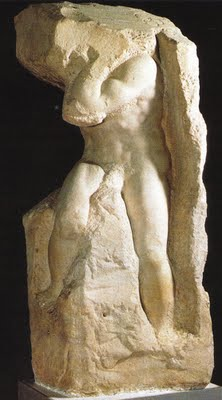
\includegraphics[width=\textwidth]{statue}\\
\tiny \flushright 
The Atlas Slave\\(Accademia, Florence)
\end{column}
\end{columns}
\end{frame}

\section{Structural Priors}

%%%%%%%%%%%%%%%%%

\begin{frame}{Typical Convolutional Layer}
\begin{figure}
   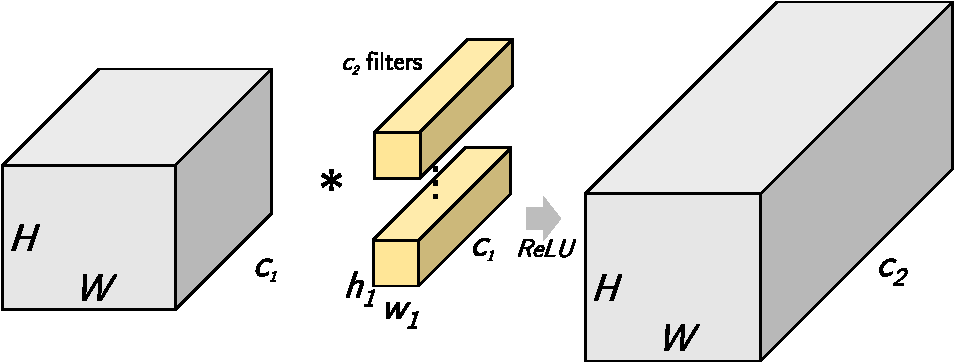
\includegraphics[width=0.9\textwidth, page=1]{../Figs/PDF/groupfig}
%   \caption{A full rank convolutional layer.}
\end{figure}
\begin{figure}

   \resizebox {0.5\textwidth} {!} {
   \begin{tikzpicture}[
       decoration={
          markings,
          mark=at position 1 with {\arrow[scale=2,gray]{latex}};
        }]
        % draw featuremap
        \pgfmathsetmacro{\cubex}{2}
        \pgfmathsetmacro{\cubey}{2}
        \pgfmathsetmacro{\cubez}{1.5}
        \draw[black,fill=fmcolor] (0,0,0) -- ++(-\cubex,0,0) -- ++(0,-\cubey,0) -- ++(\cubex,0,0) -- cycle;
        \draw[black,fill=fmshade] (0,0,0) -- ++(0,0,-\cubez) -- ++(0,-\cubey,0) -- ++(0,0,\cubez) -- cycle;
        \draw[black,fill=fmcolor] (0,0,0) -- ++(-\cubex,0,0) -- ++(0,0,-\cubez) -- ++(\cubex,0,0) -- cycle;
        \draw (-0.7, -2.5) node {image/feature map};
        
        \draw (1, -0.7) node {\LARGE$*$};
        
        % draw filter
        \pgfmathsetmacro{\cubex}{0.3}
        \pgfmathsetmacro{\cubey}{0.3}
        \pgfmathsetmacro{\cubez}{1.5}
        \draw[black,fill=filtercolor] (2,-0.7,0) -- ++(-\cubex,0,0) -- ++(0,-\cubey,0) -- ++(\cubex,0,0) -- cycle;
        \draw[black,fill=filtershade] (2,-0.7,0) -- ++(0,0,-\cubez) -- ++(0,-\cubey,0) -- ++(0,0,\cubez) -- cycle;
        \draw[black,fill=filtercolor] (2,-0.7,0) -- ++(-\cubex,0,0) -- ++(0,0,-\cubez) -- ++(\cubex,0,0) -- cycle;
        \draw (2.2, -2.5) node {filter};
            
        % draw output featuremap
        \pgfmathsetmacro{\cubex}{2}
        \pgfmathsetmacro{\cubey}{2}
        \pgfmathsetmacro{\cubez}{0.1}
        \draw[black,fill=fmcolor] (6,0,-0.75) -- ++(-\cubex,0,0) -- ++(0,-\cubey,0) -- ++(\cubex,0,0) -- cycle;
        \draw[black,fill=fmshade] (6,0,-0.75) -- ++(0,0,-\cubez) -- ++(0,-\cubey,0) -- ++(0,0,\cubez) -- cycle;
        \draw[black,fill=fmcolor] (6,0,-0.75) -- ++(-\cubex,0,0) -- ++(0,0,-\cubez) -- ++(\cubex,0,0) -- cycle;
        \draw (-0.7, -2.5) node {image/feature map};
        
        \draw[gray,postaction={decorate}] (2.7,-0.7) -- (3.8, -0.7);
        
        \draw (5.2, -2.5) node {output featuremap};
    \end{tikzpicture}
    }
\end{figure}
    \note[item]{We show here a typical convolutional layer.}
    \note[item]{Yellow blocks are filters.}
    \note[item]{Grey blocks are images or feature maps.}
\end{frame}

%%%%%%%%%%%%%%%%%%%%
\begin{frame}{Sparsity of Convolution}
\begin{figure}
    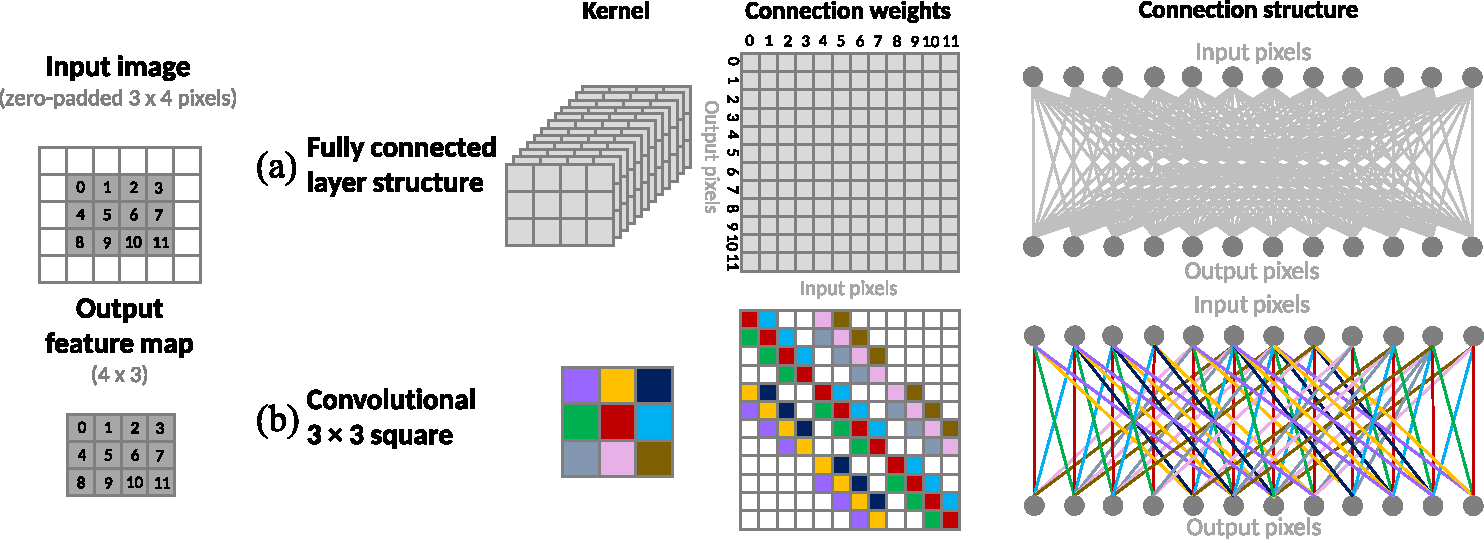
\includegraphics[width=\textwidth]{../Figs/PDF/sparseconn4}
\end{figure}
    \begin{itemize}
        \item Convolutional Neural Networks (CNNs) are structural priors for natural images
        \item Local connectivity - local correlations are important in natural images, \eg edges
        \item Shared parameters - we know we don't need to re-learn filters for every pixel
    \end{itemize}
\end{frame}
%%%%%%%%%%%%%%%%%%%%
\begin{frame}{Why are CNNs uniformly structured?}
\begin{quote}
``The marvelous powers of the brain emerge not from any single, uniformly structured
connectionist network but from highly evolved arrangements of smaller, specialized
networks which are interconnected in very specific ways.''\\
\flushright{\normalfont Marvin Minsky\\Perceptrons (1988 edition)}
\end{quote}
\begin{itemize}
    \item Deep networks are largely monolithic (uniformly connected), with few exceptions
    \item Why don't we try to structure our networks closer to the specialized components required for learning images?
\end{itemize}
\end{frame}

%%%%%%%%%%%%%%%%%%%%
\begin{frame}{Inception: Learning a Basis for Filter Size}{}
\begin{itemize}
   \item In \footcite{Szegedy2014going}, linear combination of different sized filters is learned, \ie a basis space for filters:
\end{itemize}
    
\begin{itemize}
    %\item Learns a limited number of large filters (7$\times$7, 5$\times$5), and a great number of small filters (3$\times$3, 1$\times$1)
    \item Motivation: expect most image correlations to be highly localized, \ie many small filters. However, a few may require larger, more complex filters
    %\item We can learn an effective filter of full size, but limited parameterization, by learning a basis -- the 1$\times$1 filters can learn a linear combination of the basis
\end{itemize}
\end{frame}
%%%%%%%%%%%%%%%%%%%%
\subsection{Spatial Structural Priors}

\usebackgroundtemplate{%             declare it
\tikz[overlay,remember picture] \node[opacity=0.7, at=(current page.center), yshift=-7cm] {
   \setlength{\fboxsep}{0pt}\fbox{
   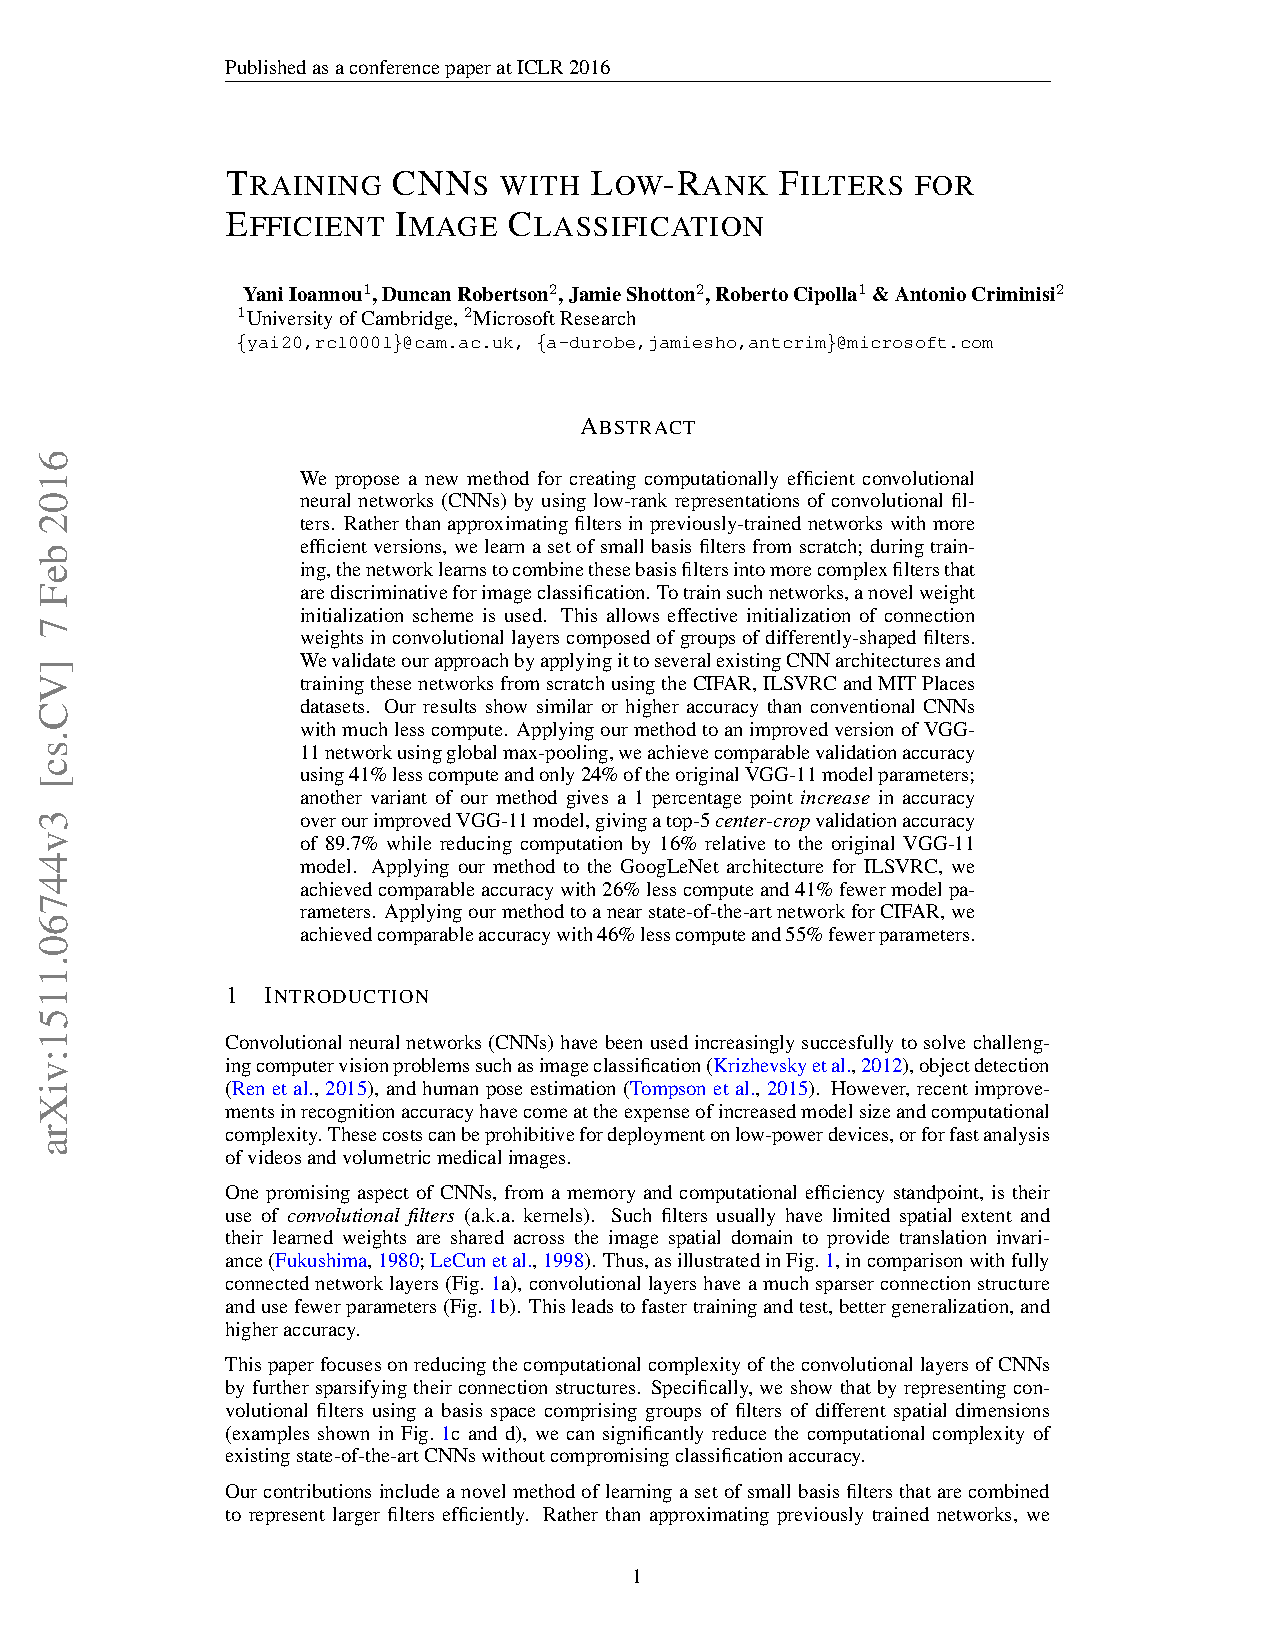
\includegraphics[width=0.9\paperwidth,page=1]{lrpaper.pdf}
   }
   };
}

\begin{frame}
\vfill
\centering
%\begin{beamercolorbox}[sep=8pt,center,shadow=true,rounded=true]{title}
\usebeamerfont{title}Spatial Structural Priors\par%
%\end{beamercolorbox}
\vfill
%Chiseling out the spatial
\end{frame}

\usebackgroundtemplate{}

%%%%%%%%%%%%%%%%%%%%
\begin{frame}{Proposed Method}{Learning a basis for filters.}
\begin{figure}
   \includegraphics[width=\textwidth, page=4]{../Figs/PDF/sparsification}
\end{figure}
\begin{itemize}
    \item A learned basis of vertical/horizontal rectangular filters and square filters!
    \item Shape of learned filters is a full $w \times h \times c$.
    \item But what can be effectively learned is limited by the number and complexity of the components.
\end{itemize}
\end{frame}

%%%%%%%%%%%%%%%%%%%%
\begin{frame}{VGG/Imagenet Results}
\centering
\pgfplotstableread[col sep=comma]{../lrdata/vggma.csv}\datatable
\pgfplotsset{major grid style={dotted,red}}

\tikzstyle{every node}=[font=\footnotesize]
\begin{tikzpicture}
\begin{axis}[
  width=\textwidth,
  height=0.4\textwidth,
  axis x line=bottom,
  ylabel=Top-5 Error,
  xlabel=Multiply-Accumulate Operations,
  axis lines=left,
  enlarge x limits=0.10,
  grid=major,
  %xmin=0,
  ytick={0.01,0.02,...,0.21},
  ymin=0.1,ymax=0.15,
  yticklabel={\pgfmathparse{\tick*100}\pgfmathprintnumber{\pgfmathresult}\%},style={
        /pgf/number format/fixed,
        /pgf/number format/precision=1
  },
  legend style={at={(0.01,0.98)}, anchor=north west, column sep=0.5em},
  legend columns=2,
]
\addplot[mark=square*,mark options={fill=blue},nodes near coords,only marks,
   point meta=explicit symbolic,
   x filter/.code={
       \ifnum\coordindex>2\def\pgfmathresult{}\fi
   },
] table[meta=Network,x=Multiply-Acc.,y expr={1 - \thisrow{Top-5 Acc.} },]{\datatable};
\addplot[mark=*,mark options={fill=green},nodes near coords,only marks,
   point meta=explicit symbolic,
   x filter/.code={
       \ifnum\coordindex<3\def\pgfmathresult{}\fi
   },
] table[meta=Network,x=Multiply-Acc.,y expr={1 - \thisrow{Top-5 Acc.} },]{\datatable};
\legend{Baseline Networks, Our Results}
\end{axis}
\end{tikzpicture}
\begin{tikzpicture}
\begin{axis}[
  width=\textwidth,
  height=0.4\textwidth,
  axis x line=bottom,
  ylabel=Top-5 Error,
  xlabel=Parameters,
  axis lines=left,
  enlarge x limits=0.10,
  grid=major,
  %xmin=0,
  ytick={0.01,0.02,...,0.21},
  ymin=0.1,ymax=0.15,
  yticklabel={\pgfmathparse{\tick*100}\pgfmathprintnumber{\pgfmathresult}\%},style={
        /pgf/number format/fixed,
        /pgf/number format/precision=1
  },
  legend style={at={(0.01,0.98)}, anchor=north west, column sep=0.5em},
  legend columns=2,
]
\addplot[mark=square*,mark options={fill=blue},nodes near coords,only marks,
   point meta=explicit symbolic,
   x filter/.code={
       \ifnum\coordindex>2\def\pgfmathresult{}\fi
   },
] table[meta=Network,x=Param.,y expr={1 - \thisrow{Top-5 Acc.} },]{\datatable};
\addplot[mark=*,mark options={fill=green},nodes near coords,only marks,
   point meta=explicit symbolic,
   x filter/.code={
       \ifnum\coordindex<3\def\pgfmathresult{}\fi
   },
] table[meta=Network,x=Param.,y expr={1 - \thisrow{Top-5 Acc.} },]{\datatable};
%\legend{Baseline Networks, Our Results}
\end{axis}
\end{tikzpicture}
%\caption{\textbf{VGG ILSVRC Results.} Multiply-accumulate operations \vs top-5 error for VGG-derived models on ILSVRC object classification dataset, the most efficient networks are closer to the origin. Our models are significantly faster than the baseline network, in the case of `gmp-lr-2x' by a factor of almost 60\%, while slightly lowering error. Note that the `gmp-lr' and `gmp-lr-join' networks have the same accuracy, showing that an explicit linear combination layer may be unnecessary.}

\end{frame}
%%%%%%%%%%%%%%%%%%%%

\begin{frame}{Imagenet Results}

%Applying our method to an improved version of VGG-11 network using global max-pooling, we achieve comparable validation accuracy using 41% less compute and only 24% of the original VGG-11 model parameters; another variant of our method gives a 1 percentage point increase in accuracy over our improved VGG-11 model, giving a top-5 center-crop validation accuracy of 89.7% while reducing computation by 16% relative to the original VGG-11 model. Applying our method to the GoogLeNet architecture for ILSVRC, we achieved comparable accuracy with 26% less compute and 41% fewer model parameters.
%Applying our method to a near state-of-the-art network for CIFAR, we achieved comparable accuracy with 46% less compute and 55% fewer parameters. Networks with root modules have similar or higher accuracy than the baseline architectures with much less computation.
\begin{itemize}
    \item VGG-11 (low-rank): \textbf{24\%} smaller, \textbf{41\%} fewer FLOPS
    \item VGG-11 (low-rank/full-rank mix): \textbf{16\%} fewer FLOPS with \textbf{1\% lower error} on ILSRVC val, but 16\% larger.
    \item GoogLeNet: \textbf{41\%} smaller, \textbf{26\%} fewer FLOPS
\end{itemize}
\vfill
Or better results if you tune it on GoogLeNet more\ldots
\end{frame}
%%%%%%%%%%%%%%%%%%%%

\usebackgroundtemplate{
\tikz[overlay,remember picture] \node[opacity=0.5, at=(current page.center), yshift=-1cm] {
\centering
   \setlength{\fboxsep}{0pt}\setlength\fboxrule{0.5pt}\fbox{
   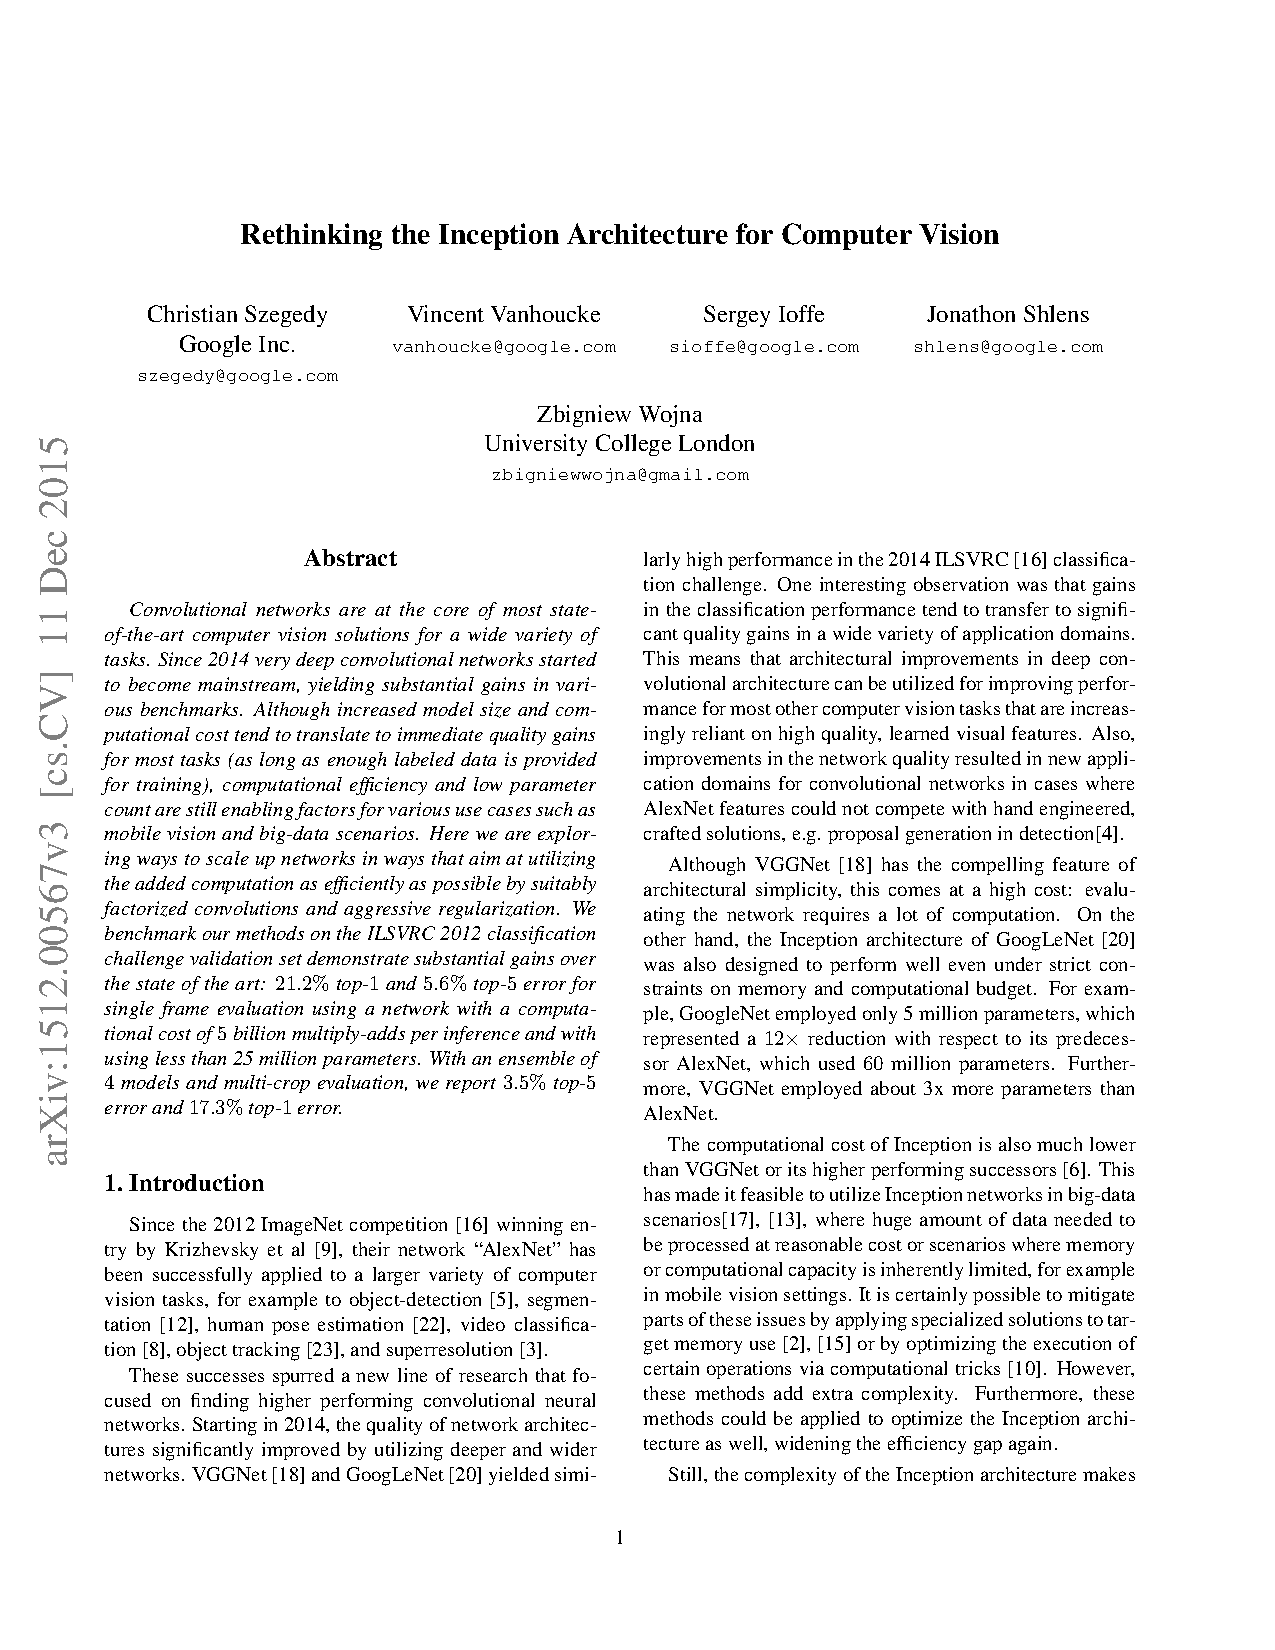
\includegraphics[width=0.9\paperwidth,page=1]{inceptionv3.pdf}
   }
   };
}

\begin{frame}
\vfill
\centering
\colorbox{white}{
\setlength{\fboxsep}{0pt}\fbox{
\begin{minipage}{0.6\paperwidth}
   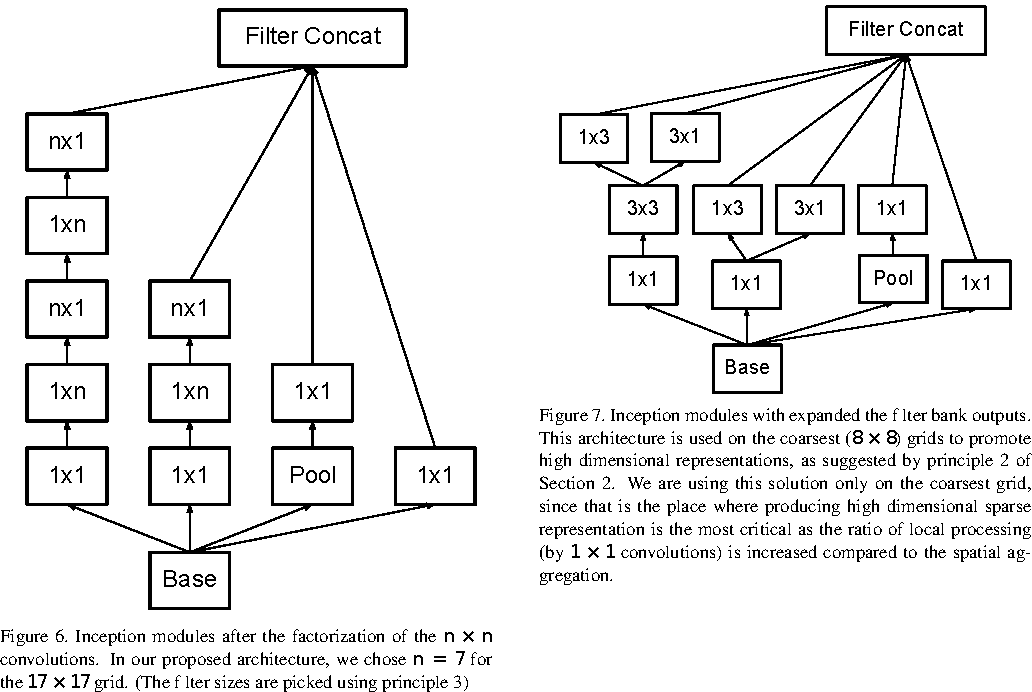
\includegraphics[width=0.6\paperwidth,page=1]{inceptionv3-filterconfig.pdf}
\end{minipage}}}
\end{frame}

\usebackgroundtemplate{}

%%%%%%%%%%%%%%%%%%%%

\subsection{Filter-wise Structural Priors}

\usebackgroundtemplate{%             declare it
\tikz[overlay,remember picture] \node[opacity=0.7, at=(current page.center), yshift=-7cm] {
   \setlength{\fboxsep}{0pt}\fbox{
   \includegraphics[width=0.9\paperwidth,page=1]{deeproots.pdf}
   }
   };
}

\begin{frame}
\vfill
\centering
%\begin{beamercolorbox}[sep=8pt,center,shadow=true,rounded=true]{title}
\usebeamerfont{title}Filter-wise Structural Priors\par%
%\end{beamercolorbox}
\vfill
\end{frame}

\usebackgroundtemplate{}

%%%%%%%%%%%%%%%%%%%%
\begin{frame}{Typical Convolutional Layer}
\begin{figure}
   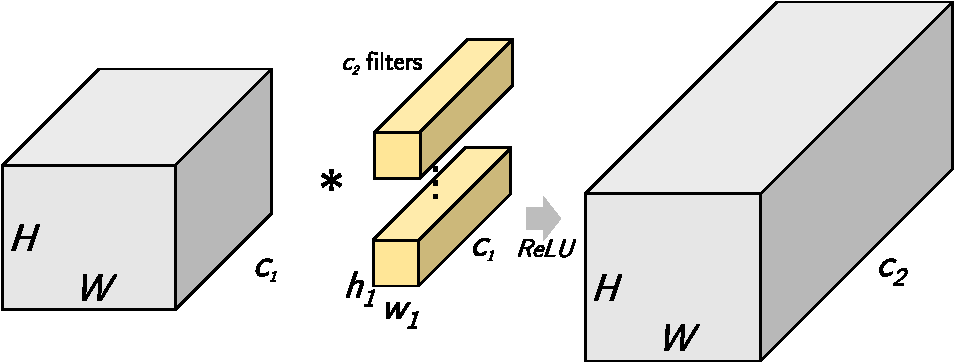
\includegraphics[width=0.9\textwidth, page=1]{../Figs/PDF/groupfig}
%   \caption{A full rank convolutional layer.}
\end{figure}
\begin{figure}

   \resizebox {0.5\textwidth} {!} {
   \begin{tikzpicture}[
       decoration={
          markings,
          mark=at position 1 with {\arrow[scale=2,gray]{latex}};
        }]
        % draw featuremap
        \pgfmathsetmacro{\cubex}{2}
        \pgfmathsetmacro{\cubey}{2}
        \pgfmathsetmacro{\cubez}{1.5}
        \draw[black,fill=fmcolor] (0,0,0) -- ++(-\cubex,0,0) -- ++(0,-\cubey,0) -- ++(\cubex,0,0) -- cycle;
        \draw[black,fill=fmshade] (0,0,0) -- ++(0,0,-\cubez) -- ++(0,-\cubey,0) -- ++(0,0,\cubez) -- cycle;
        \draw[black,fill=fmcolor] (0,0,0) -- ++(-\cubex,0,0) -- ++(0,0,-\cubez) -- ++(\cubex,0,0) -- cycle;
        \draw (-0.7, -2.5) node {image/feature map};
        
        \draw (1, -0.7) node {\LARGE$*$};
        
        % draw filter
        \pgfmathsetmacro{\cubex}{0.3}
        \pgfmathsetmacro{\cubey}{0.3}
        \pgfmathsetmacro{\cubez}{1.5}
        \draw[black,fill=filtercolor] (2,-0.7,0) -- ++(-\cubex,0,0) -- ++(0,-\cubey,0) -- ++(\cubex,0,0) -- cycle;
        \draw[black,fill=filtershade] (2,-0.7,0) -- ++(0,0,-\cubez) -- ++(0,-\cubey,0) -- ++(0,0,\cubez) -- cycle;
        \draw[black,fill=filtercolor] (2,-0.7,0) -- ++(-\cubex,0,0) -- ++(0,0,-\cubez) -- ++(\cubex,0,0) -- cycle;
        \draw (2.2, -2.5) node {filter};
            
        % draw output featuremap
        \pgfmathsetmacro{\cubex}{2}
        \pgfmathsetmacro{\cubey}{2}
        \pgfmathsetmacro{\cubez}{0.1}
        \draw[black,fill=fmcolor] (6,0,-0.75) -- ++(-\cubex,0,0) -- ++(0,-\cubey,0) -- ++(\cubex,0,0) -- cycle;
        \draw[black,fill=fmshade] (6,0,-0.75) -- ++(0,0,-\cubez) -- ++(0,-\cubey,0) -- ++(0,0,\cubez) -- cycle;
        \draw[black,fill=fmcolor] (6,0,-0.75) -- ++(-\cubex,0,0) -- ++(0,0,-\cubez) -- ++(\cubex,0,0) -- cycle;
        \draw (-0.7, -2.5) node {image/feature map};
        
        \draw[gray,postaction={decorate}] (2.7,-0.7) -- (3.8, -0.7);
        
        \draw (5.2, -2.5) node {output featuremap};
    \end{tikzpicture}
    }
\end{figure}
    \note[item]{We show here a typical convolutional layer.}
    \note[item]{Yellow blocks are filters.}
    \note[item]{Grey blocks are images or feature maps.}
\end{frame}

%%%%%%%%%%%%%%%%%%%
\begin{frame}{AlexNet Filter Grouping}
\begin{figure}
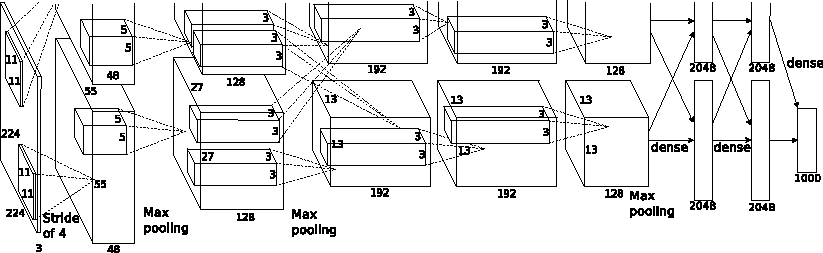
\includegraphics[width=\columnwidth]{alexnet}
\end{figure}
\begin{itemize}
\item Uses 2 filter groups in most of the convolutional layers
\item Allowed training across two GPUs (model parallelism)
\end{itemize}
\end{frame}

%%%%%%%%%%%%%%%%%%%

\begin{frame}{AlexNet Filter Grouping}
	\centering
    \begin{figure}
    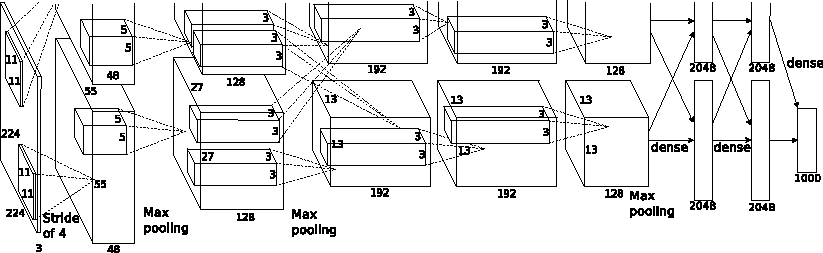
\includegraphics[width=0.9\columnwidth]{alexnet}
    \end{figure}
	\pgfplotstableread[col sep=comma]{../rootdata/alexnetma.csv}\datatable
	\pgfplotsset{major grid style={dotted,red}}
	
	\begin{tikzpicture}
	\begin{axis}[
	width=\linewidth,
	height=0.4\linewidth,
	axis x line=bottom,
	ylabel=Top-5 Val.\ Error,
	xlabel=Model Parameters (\# floats),
	axis lines=left,
	enlarge x limits=0.12,
	enlarge y limits=0.1,
	grid=major,
	%xmin=0,
	ytick={0.01,0.02,...,0.21},
	ymin=0.18,ymax=0.2,
	yticklabel={\pgfmathparse{\tick*100}\pgfmathprintnumber{\pgfmathresult}\%},style={
		/pgf/number format/fixed,
		/pgf/number format/precision=1
	},
	legend style={at={(0.98,0.98)}, anchor=north east, column sep=0.5em},
	legend columns=2,
	]
	\addplot[mark=*,mark options={fill=black},nodes near coords,only marks,
	point meta=explicit symbolic,
	] table[meta=Network,x=Param.,y expr={1 - \thisrow{Top-5 Acc.} },]{\datatable};
	\end{axis}
	\end{tikzpicture}
	\end{frame}

%%%%%%%%%%%%%%%%%%%%

\begin{frame}{Grouped Convolutional Layer}
\begin{figure}
   \includegraphics[width=0.9\textwidth, page=2]{../Figs/PDF/groupfig}
%   \caption{A full rank convolutional layer.}
\end{figure}
\begin{figure}

   \resizebox {0.5\textwidth} {!} {
   \begin{tikzpicture}[
       decoration={
          markings,
          mark=at position 1 with {\arrow[scale=2,gray]{latex}};
        }]
        % draw featuremap
        \pgfmathsetmacro{\cubex}{2}
        \pgfmathsetmacro{\cubey}{2}
        \pgfmathsetmacro{\cubez}{1.5}
        \draw[black,fill=fmcolor] (0,0,0) -- ++(-\cubex,0,0) -- ++(0,-\cubey,0) -- ++(\cubex,0,0) -- cycle;
        \draw[black,fill=fmshade] (0,0,0) -- ++(0,0,-\cubez) -- ++(0,-\cubey,0) -- ++(0,0,\cubez) -- cycle;
        \draw[black,fill=fmcolor] (0,0,0) -- ++(-\cubex,0,0) -- ++(0,0,-\cubez) -- ++(\cubex,0,0) -- cycle;
        \draw (-0.7, -2.5) node {image/feature map};
        
        \draw (1, -0.7) node {\LARGE$*$};
        
        % draw filter
        \pgfmathsetmacro{\cubex}{0.3}
        \pgfmathsetmacro{\cubey}{0.3}
        \pgfmathsetmacro{\cubez}{1.5}
        \draw[black,fill=filtercolor] (2,-0.7,0) -- ++(-\cubex,0,0) -- ++(0,-\cubey,0) -- ++(\cubex,0,0) -- cycle;
        \draw[black,fill=filtershade] (2,-0.7,0) -- ++(0,0,-\cubez) -- ++(0,-\cubey,0) -- ++(0,0,\cubez) -- cycle;
        \draw[black,fill=filtercolor] (2,-0.7,0) -- ++(-\cubex,0,0) -- ++(0,0,-\cubez) -- ++(\cubex,0,0) -- cycle;
        \draw (2.2, -2.5) node {filter};
            
        % draw output featuremap
        \pgfmathsetmacro{\cubex}{2}
        \pgfmathsetmacro{\cubey}{2}
        \pgfmathsetmacro{\cubez}{0.1}
        \draw[black,fill=fmcolor] (6,0,-0.75) -- ++(-\cubex,0,0) -- ++(0,-\cubey,0) -- ++(\cubex,0,0) -- cycle;
        \draw[black,fill=fmshade] (6,0,-0.75) -- ++(0,0,-\cubez) -- ++(0,-\cubey,0) -- ++(0,0,\cubez) -- cycle;
        \draw[black,fill=fmcolor] (6,0,-0.75) -- ++(-\cubex,0,0) -- ++(0,0,-\cubez) -- ++(\cubex,0,0) -- cycle;
        \draw (-0.7, -2.5) node {image/feature map};
        
        \draw[gray,postaction={decorate}] (2.7,-0.7) -- (3.8, -0.7);
        
        \draw (5.2, -2.5) node {output featuremap};
    \end{tikzpicture}
    }
\end{figure}
    \note[item]{We show here a grouped convolutional layer.}
    \note[item]{Yellow blocks are filters.}
    \note[item]{Grey blocks are images or feature maps.}
\end{frame}

%%%%%%%%%%%%%%%%%%%%

\begin{frame}{Root Modules}
%\includegraphics[width=0.7\linewidth, page=4]{../Figs/PDF/groupfig}
%   \caption{Convolution with $d$ filters of shape $h\times w\times c$.}
%   \label{fig:normalresnet}
%\end{subfigure}\\
%\begin{subfigure}[t]{\linewidth}
\centering
\includegraphics[width=0.9\linewidth, page=5]{../Figs/PDF/groupfig}\\
Root-2 Module: $d$ filters in $g = 2$ filter groups, of shape $h\times w\times c/2$.
\includegraphics[width=0.9\linewidth, page=6]{../Figs/PDF/groupfig}\\
Root-4 Module: $d$ filters in $g = 4$ filter groups, of shape $h\times w\times c/4$.
\end{frame}

%%%%%%%%%%%%%%%%%%%

\begin{frame}{Network-in-Network}
            \centering
			\begin{tikzpicture}[ampersand replacement=\&]
			\begin{scope}[]
			\matrix[column sep=0em]{
				\node (1a) {
					\includegraphics[height=0.12\linewidth, page=15]{../Figs/PDF/groupfig}
				};\&
				\node (1b) {
					\includegraphics[height=0.145\linewidth, page=17]{../Figs/PDF/groupfig}
				};\& 
				\node (1c) {
					\includegraphics[height=0.145\linewidth, page=17]{../Figs/PDF/groupfig}
				};\&
				\node (1cdots) {
					{\Large $\cdots$}
				};\\
				\draw node{{\footnotesize \textit{input}} \hspace{0.05em} {\footnotesize \textit{conv1a}}};\&
				\draw node{\footnotesize \textit{conv1b}};\&
				\draw node{\footnotesize \textit{conv1c}};\\
				\node (2adots) {
					{\Large $\cdots$}
				};\&
				\node (2a) {
				    \includegraphics[height=0.12\linewidth, page=16]{../Figs/PDF/groupfig}
				};\&
				\node (2b) {
					\includegraphics[height=0.145\linewidth, page=17]{../Figs/PDF/groupfig}
				};\&
				\node (2c) {
					\includegraphics[height=0.145\linewidth, page=17]{../Figs/PDF/groupfig}
				};\&
				\node (2cdots) {
					{\Large $\cdots$}
				};\\
				\&
				\draw node{\footnotesize \textit{conv2a}};\&
				\draw node{\footnotesize \textit{conv2b}};\&
				\draw node{\footnotesize \textit{conv2c}};\\
				\node (3adots) {
					{\Large $\cdots$}
				};\&
				\node (3a) {
				    \includegraphics[height=0.12\linewidth, page=16]{../Figs/PDF/groupfig}
				};\&
				\node (3b) {
					\includegraphics[height=0.145\linewidth, page=17]{../Figs/PDF/groupfig}
				};\&
				\node (3c) {
					\includegraphics[height=0.145\linewidth, page=17]{../Figs/PDF/groupfig}
				};\&
				\node (1a) {
					\includegraphics[height=0.12\linewidth, page=20]{../Figs/PDF/groupfig}
				};\\
				\&
				\draw node{\footnotesize \textit{conv3a}};\&
				\draw node{\footnotesize \textit{conv3b}};\&
				\draw node{\footnotesize \textit{conv3c}};\&
				\draw node{\footnotesize \textit{pool} \hspace{0.08em} {\footnotesize \textit{output}}};\\
			};
			\end{scope}
			\end{tikzpicture}
\end{frame}

%%%%%%%%%%%%%%%%%%%%

\begin{frame}{NiN Root Architectures}
			\begin{tikzpicture}[ampersand replacement=\&]
			\begin{scope}[]
			\matrix[column sep=0em, row sep=2em]{
				\node (1) {
					{\Large $\cdots$}
				};\&
				\node (1c) {
					\includegraphics[height=0.11\linewidth, page=17]{../Figs/PDF/groupfig}
				};\& 
				\node (2a) {
				    \includegraphics[height=0.09\linewidth, page=16]{../Figs/PDF/groupfig}
				};\&
				\node (2b) {
					\includegraphics[height=0.11\linewidth, page=17]{../Figs/PDF/groupfig}
				};\&
				\node (2c) {
					\includegraphics[height=0.11\linewidth, page=17]{../Figs/PDF/groupfig}
				};\&
				\node (3a) {
				    \includegraphics[height=0.09\linewidth, page=16]{../Figs/PDF/groupfig}
				};\&
				\node (3b) {
					\includegraphics[height=0.11\linewidth, page=17]{../Figs/PDF/groupfig}
				};\&
				\node (4) {
					{\Large $\cdots$}
				};\\
				%%%%%%%%%%%%%%%%%%
			    
				%%%%%%%%%%%%%%%%%%
				\node (r1) {
					{\Large $\cdots$}
				};\&
				\node (r1c) {
					\includegraphics[height=0.11\linewidth, page=17]{../Figs/PDF/groupfig}
				};\& 
				\node (r2a) {
					\includegraphics[height=0.15\linewidth, page=19]{../Figs/PDF/groupfig}
				};\&
				\node (r2b) {
					\includegraphics[height=0.11\linewidth, page=17]{../Figs/PDF/groupfig}
				};\&
				\node (r2c) {
					\includegraphics[height=0.11\linewidth, page=17]{../Figs/PDF/groupfig}
				};\&
				\node (r3a) {
					\includegraphics[height=0.09\linewidth, page=18]{../Figs/PDF/groupfig}
				};\&
				\node (r3b) {
					\includegraphics[height=0.11\linewidth, page=17]{../Figs/PDF/groupfig}
				};\&
				\node (r4) {
					{\Large $\cdots$}
				};\\
			};
			\draw[->] (2a) edge (r2a);
			\draw[->] (3a) edge (r3a);
			
			\draw[decorate,decoration={brace,mirror},](r2a.south west) -- node[below=3pt] {\small root-4 module} ++(2.3, 0);
			\draw[decorate,decoration={brace,mirror},yshift=-2em](r3a.south west) + (0, -0.4) -- node[below=3pt] {\small root-2 module} ++(2.5, -0.4);
			\end{scope}
			\end{tikzpicture}
\end{frame}

%%%%%%%%%%%%%%%%%%%%
\section*{Results}

\begin{frame}{NiN Root Architectures}
\centering
\textbf{Network-in-Network}. Filter groups in each convolutional layer.
\vfill
%\resizebox{\linewidth}{!}{
\begin{tabular}{@{}lm{1.5em}m{1.5em}m{1.5em}m{1.5em}m{1.5em}m{1.5em}m{1.5em}m{1.5em}m{1.5em}@{}}
\toprule
    Model & \multicolumn{3}{c}{conv1} & \multicolumn{3}{c}{conv2} & \multicolumn{3}{c}{conv3} \\
     & \textit{\footnotesize a} & \textit{\footnotesize b} & \textit{\footnotesize c} & \textit{\footnotesize a} & \textit{\footnotesize b} & \textit{\footnotesize c} & \textit{\footnotesize a} & \textit{\footnotesize b} & \textit{\footnotesize c} \\
     & \textit{\footnotesize5$\times$5} & \textit{\footnotesize1$\times$1} & \textit{\footnotesize1$\times$1} & \textit{\footnotesize5$\times$5} & \textit{\footnotesize1$\times$1} & \textit{\footnotesize1$\times$1} & \textit{\footnotesize3$\times$3} & \textit{\footnotesize1$\times$1} & \textit{\footnotesize1$\times$1} \\
    Orig. & 1 & 1 & 1 & 1 & 1 & 1 & 1 & 1 & 1\\
    \midrule
    root-2 & 1 & 1 & 1 & 2 & 1 & 1 & 1 & 1 & 1\\
    root-4 & 1 & 1 & 1 & 4 & 1 & 1 & 2 & 1 & 1\\
    root-8 & 1 & 1 & 1 & 8 & 1 & 1 & 4 & 1 & 1\\
    root-16 & 1 & 1 & 1 & 16 & 1 & 1 & 8 & 1 & 1\\
    \bottomrule
\end{tabular}
\vfill
\end{frame}


%%%%%%%%%%%%%%%%%%%%
\begin{frame}{CIFAR10: Model Parameters \vs Error}
\footnotesize
\pgfplotstableread[col sep=comma]{../rootdata/nincifar.csv}\datatable
\pgfplotstableread[col sep=comma]{../rootdata/nincifar_root_s.csv}\rdatatable
\pgfplotstableread[col sep=comma]{../rootdata/nincifar_tree_s.csv}\tdatatable
\pgfplotstableread[col sep=comma]{../rootdata/nincifar_col_s.csv}\cdatatable
\pgfplotsset{major grid style={dotted,red}}

\centering
\begin{tikzpicture}
%\tikzstyle{every node}=[font=\footnotesize]
\begin{axis}[
  width=\linewidth,
  height=0.66\linewidth,
  axis x line=bottom,
  ylabel=Error,
  xlabel=Model Parameters,
  axis lines=left,
  enlarge x limits=0.05,
  enlarge y limits=0.05,
  grid=major,
  %xmin=0,
  ytick={0.002,0.004,...,1.0},
  %ymin=0.075,ymax=0.09,
  xticklabel style={
        /pgf/number format/fixed,
        /pgf/number format/precision=1
  },
  yticklabel={\pgfmathparse{\tick*1}\pgfmathprintnumber{\pgfmathresult}\%},style={
        /pgf/number format/fixed zerofill,
        /pgf/number format/precision=1
  },
  legend style={at={(1,0.95)}, anchor=south east, column sep=0.2em, font=\small},
  legend columns=4,
]
\addplot[mark=*,mark options={fill=red},
   %nodes near coords,
   only marks,
   point meta=explicit symbolic,
   error bars/y dir=both,
   error bars/y fixed=0.00131497782,
] table[meta=name,x=param,y expr={1 - \thisrow{accuracy} },]{\datatable};
\addplot[mark=square*,mark options={fill=green},
   nodes near coords, only marks,
   every node near coord/.append style={inner sep=4pt},
   point meta=explicit symbolic,
] table[meta=name,x=param,y expr={1 - \thisrow{accuracy} },]{\rdatatable};
\addplot[mark=triangle*,mark options={fill=blue},
   nodes near coords, nodes near coords align = {below}, only marks,
   every node near coord/.append style={inner sep=4pt},
   point meta=explicit symbolic,
] table[meta=name,x=param,y expr={1 - \thisrow{accuracy} },]{\tdatatable};
\addplot[mark=diamond*,mark options={fill=yellow},
   nodes near coords, nodes near coords align = {below}, only marks,
   every node near coord/.append style={inner sep=4pt},
   point meta=explicit symbolic,
] table[meta=name,x=param,y expr={1 - \thisrow{accuracy} },]{\cdatatable};
\legend{NiN, Root, Tree, Column}
\end{axis}
\end{tikzpicture}
%\caption{\textbf{Model Parameters \vs Error.}}
%\label{fig:nincifarparamconvonly}
{\tiny NiN: mean and standard deviation (error bars) are shown over 5 different random initializations.}
\end{frame}

\begin{frame}{CIFAR10: FLOPS (Multiply-Add) \vs Error.}
\pgfplotstableread[col sep=comma]{../rootdata/nincifar.csv}\datatable
\pgfplotstableread[col sep=comma]{../rootdata/nincifar_root_s.csv}\rdatatable
\pgfplotstableread[col sep=comma]{../rootdata/nincifar_tree_s.csv}\tdatatable
\pgfplotstableread[col sep=comma]{../rootdata/nincifar_col_s.csv}\cdatatable
\pgfplotsset{major grid style={dotted,red}}
\footnotesize

\centering
\begin{tikzpicture}
%\tikzstyle{every node}=[font=\footnotesize]
\begin{axis}[
  width=\linewidth,
  height=0.66\linewidth,
  axis x line=bottom,
  ylabel=Error,
  xlabel=FLOPS (Multiply-Add),
  axis lines=left,
  enlarge x limits=0.05,
  enlarge y limits=0.05,
  grid=major,
  %xmin=0,
  ytick={0.002,0.004,...,1.0},
  %ymin=0.075,ymax=0.09,
  xticklabel style={
        /pgf/number format/fixed zerofill,
        /pgf/number format/precision=1
  },
  yticklabel={\pgfmathparse{\tick*1}\pgfmathprintnumber{\pgfmathresult}\%},style={
        /pgf/number format/fixed zerofill,
        /pgf/number format/precision=1
  },
  legend style={at={(1,0.95)}, anchor=south east, column sep=0.2em, font=\small},
  legend columns=4,
]
\addplot[mark=*,mark options={fill=red},
   %nodes near coords,
   only marks,
   point meta=explicit symbolic,
   error bars/y dir=both,
   error bars/y fixed=0.00131497782,
] table[meta=name,x=ma,y expr={1 - \thisrow{accuracy} },]{\datatable};
\addplot[mark=square*,mark options={fill=green},
   nodes near coords, only marks,
   every node near coord/.append style={inner sep=4pt},
   point meta=explicit symbolic,
] table[meta=name,x=ma,y expr={1 - \thisrow{accuracy} },]{\rdatatable};
\addplot[mark=triangle*,mark options={fill=blue},
   nodes near coords, nodes near coords align = {below}, only marks,
   every node near coord/.append style={inner sep=4pt},
   point meta=explicit symbolic,
] table[meta=name,x=ma,y expr={1 - \thisrow{accuracy} },]{\tdatatable};
\addplot[mark=diamond*,mark options={fill=yellow},
   nodes near coords, nodes near coords align = {below}, only marks,
   every node near coord/.append style={inner sep=4pt},
   point meta=explicit symbolic,
] table[meta=name,x=ma,y expr={1 - \thisrow{accuracy} },]{\cdatatable};
\legend{NiN, Root, Tree, Column}
\end{axis}
\end{tikzpicture}
{\tiny NiN: mean and standard deviation (error bars) are shown over 5 different random initializations.}
%\caption{\textbf{FLOPS (Multiply-Add) \vs Error.}}
%\label{fig:nincifarmaconvonly}

%\caption{\textbf{Network-in-Network CIFAR10 Results.} Spatial filters (3$\times$3, 5$\times$5) are grouped hierarchically. The best models are closest to the origin. 
%(left) Parameters \vs Error, (right) FLOPS \vs Error.}

\end{frame}
%%%%%%%%%%%%%%%%%%%%


\newcommand{\covarlabels}[1]{%
\tiny
\vspace{0.75em}
\begin{tikzpicture}[remember picture]
\node [anchor=south west, inner sep=0pt] (c)
    {
        #1
    };
    \path[use as bounding box] (c.south west) rectangle (c.north east);
    \node [anchor=south west, xshift=-0.5em, yshift=-0.5em, rotate=45] at (c.north west) {\footnotesize 0};
    \node [anchor=south east, xshift=\linewidth, yshift=-0.2em] at (c.north west) {\footnotesize 192};
    \node [anchor=south west, xshift=0.25em, yshift=-1.05\linewidth, rotate=90] at (c.north west) {\footnotesize 192};
    \node [anchor=south, xshift=0.5\linewidth] at (c.north west) {\footnotesize\texttt{conv3a}};
    \node [anchor=south, xshift=0.2em, yshift=-0.5\linewidth, rotate=90] at (c.north west) {\footnotesize \texttt{conv2c}};
\end{tikzpicture}%
}

\begin{frame}{Inter-layer Filter Covariance}

\begin{figure}[tb]
\centering
\begin{subfigure}[b]{0.31\linewidth}
\centering
    \covarlabels{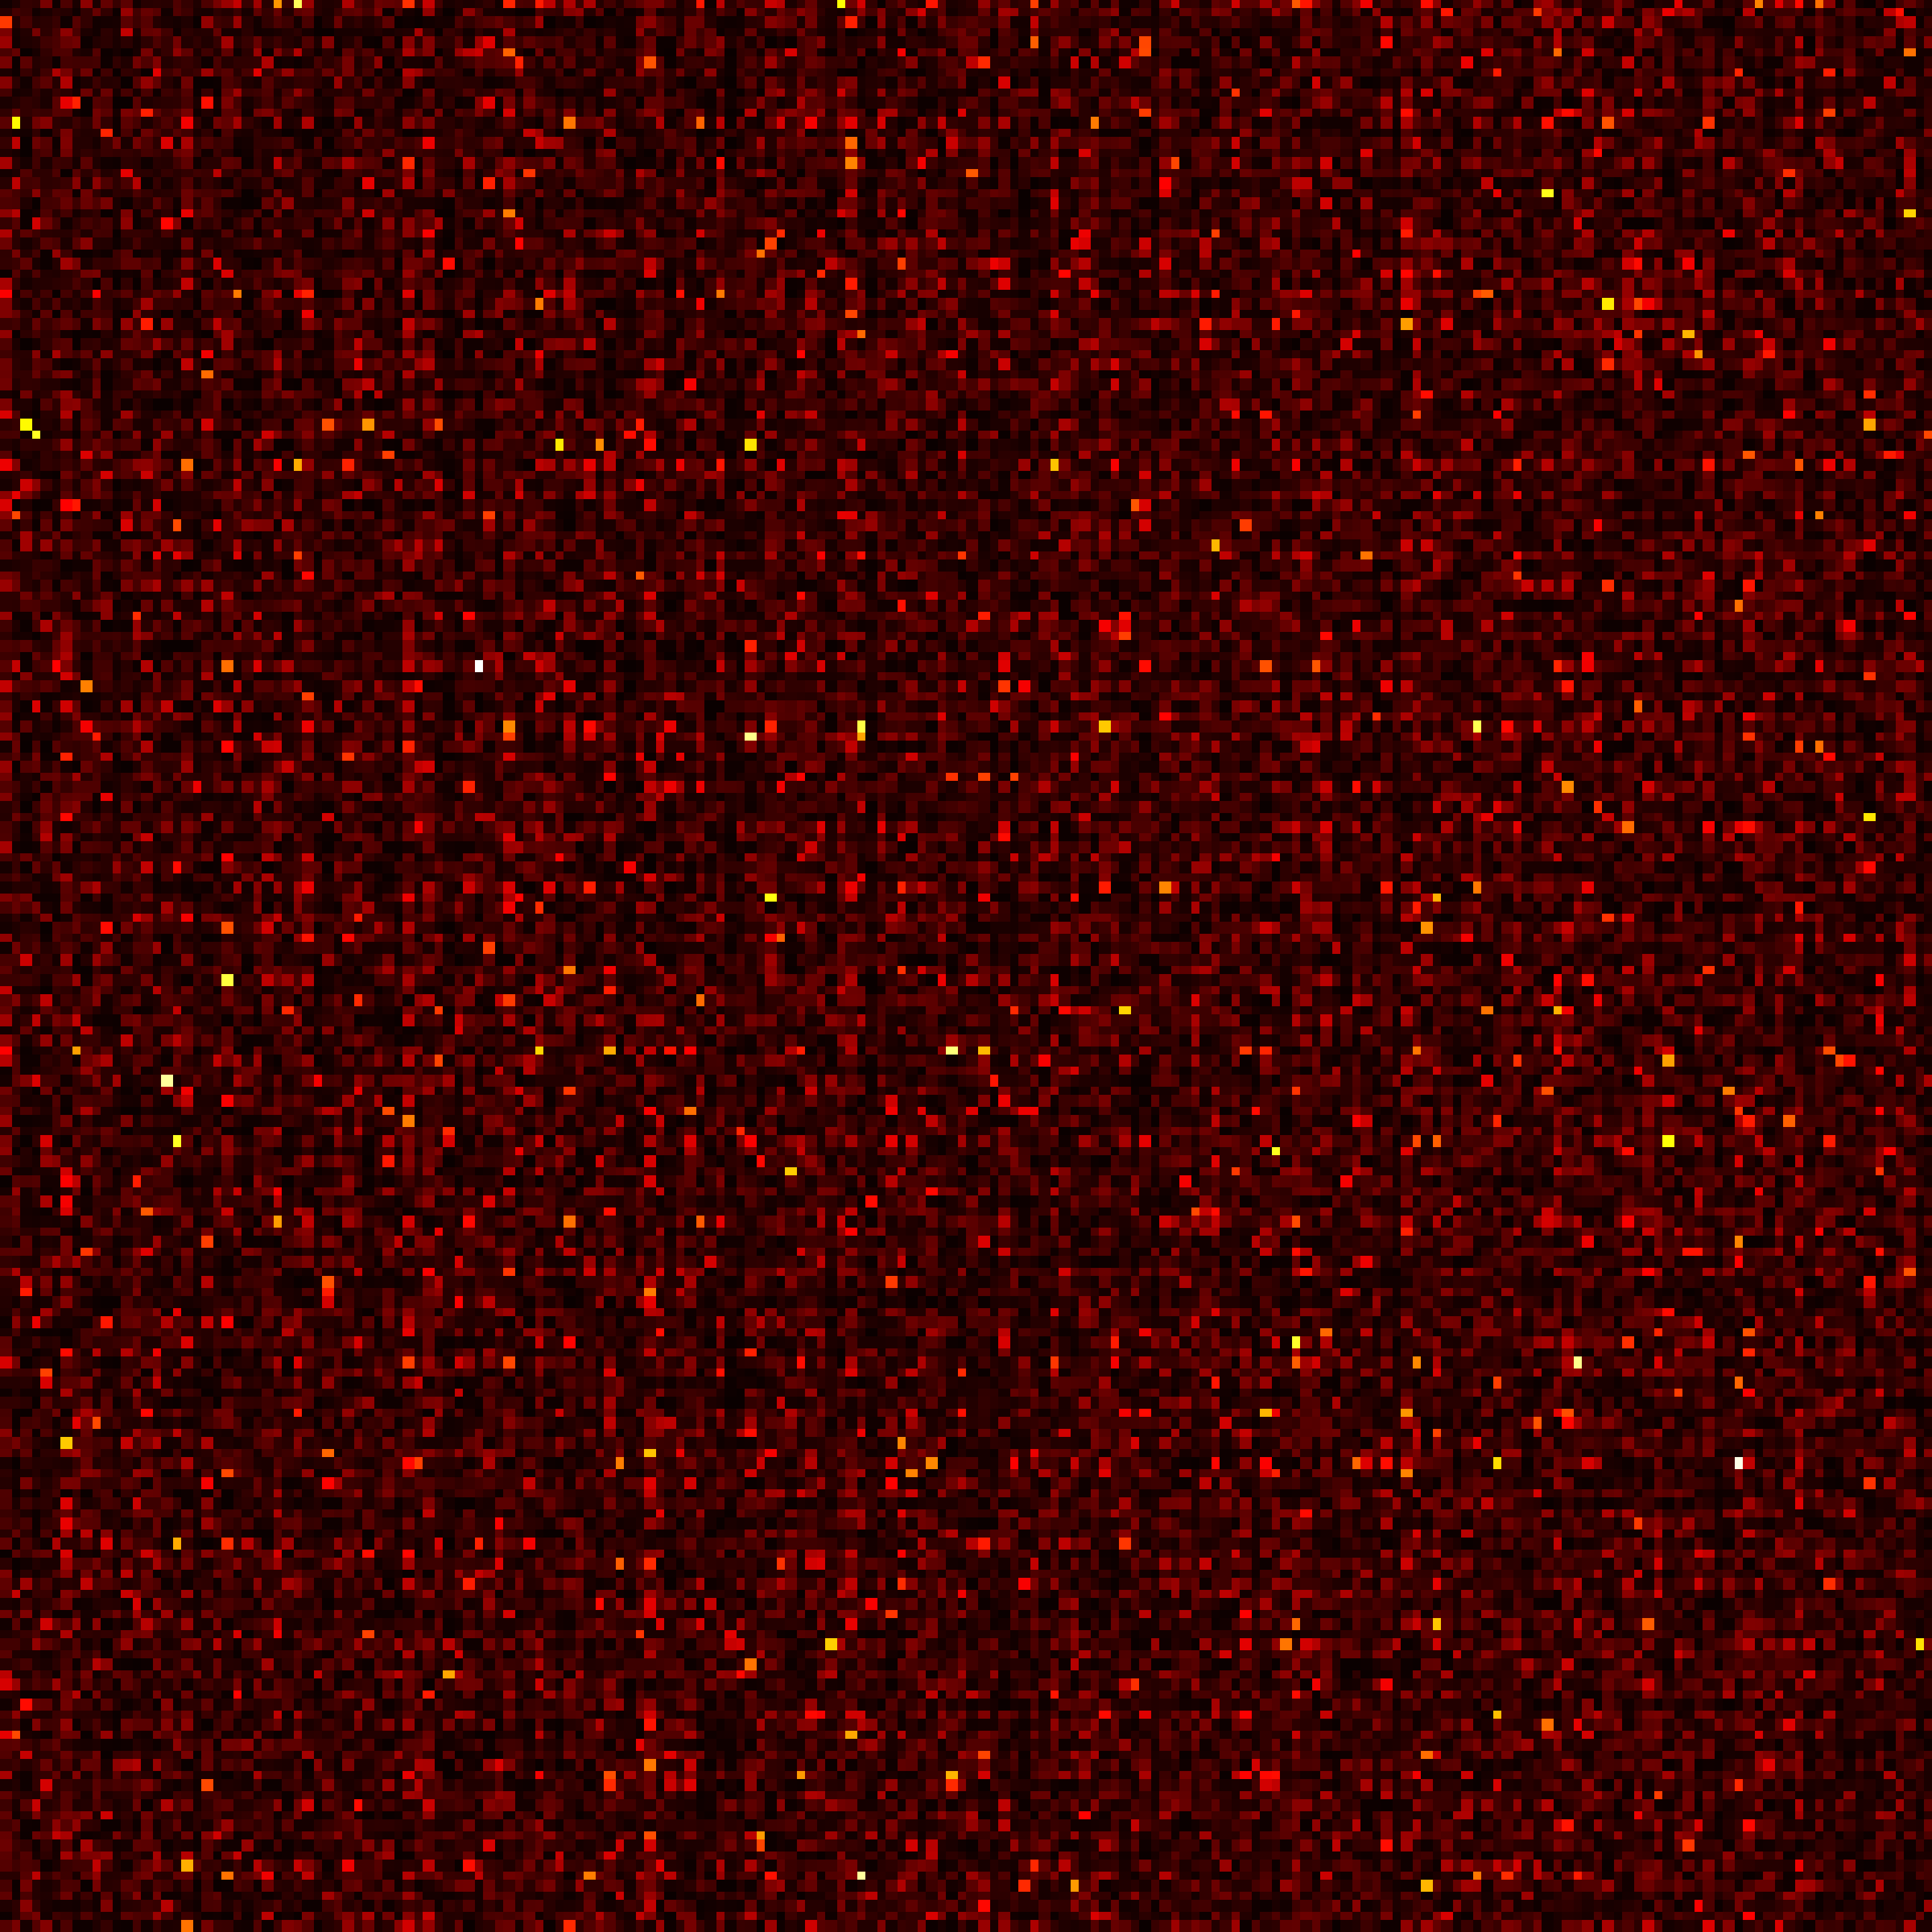
\includegraphics[width=\linewidth]{../Figs/Raster/msrc-cifar-nin-4pad-conv8-corr}}
    \caption{\textbf{Standard:} $g=1$}
    \label{fig:normalcovartest}
\end{subfigure}
~
\begin{subfigure}[b]{0.31\linewidth}
\centering
    \covarlabels{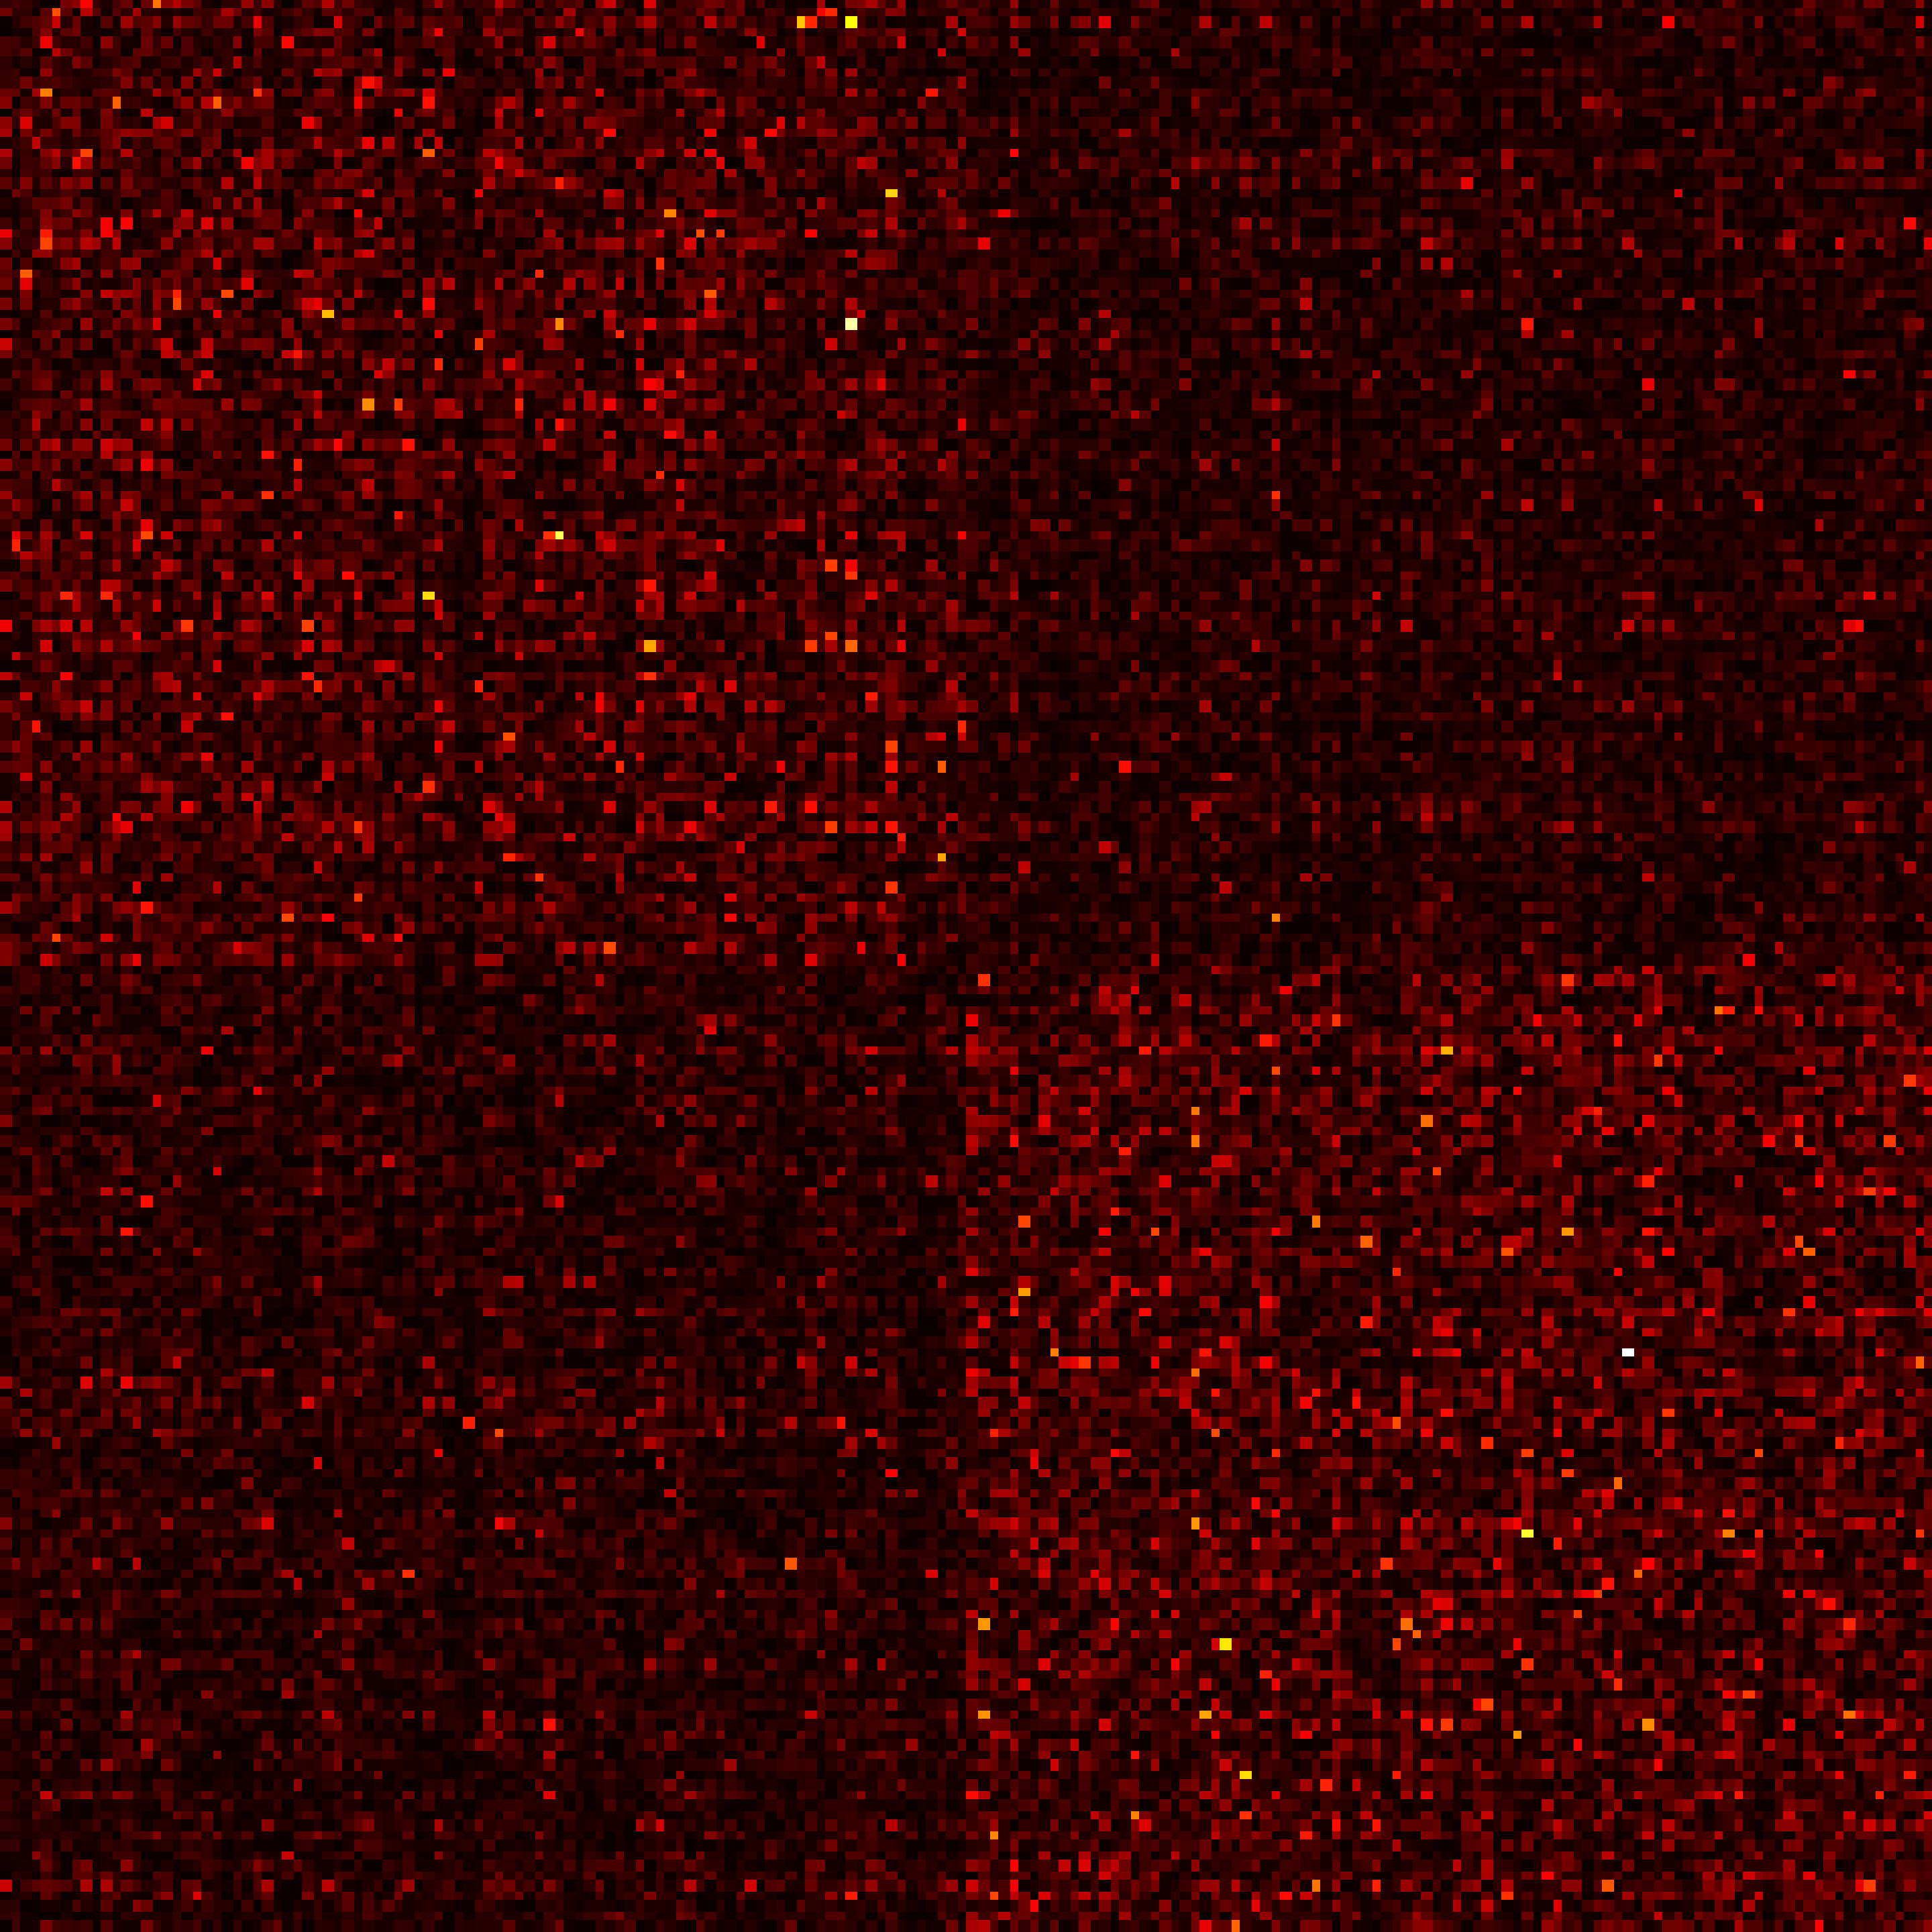
\includegraphics[width=\linewidth]{../Figs/Raster/msrc-cifar-nin-4pad-funnel4-convonly-conv8-corr}}
    \caption{\textbf{Root-4:} $g=2$}
    \label{fig:root4}
\end{subfigure}
%~
%\begin{subfigure}[b]{0.24\linewidth}
%\centering
%    \covarlabels{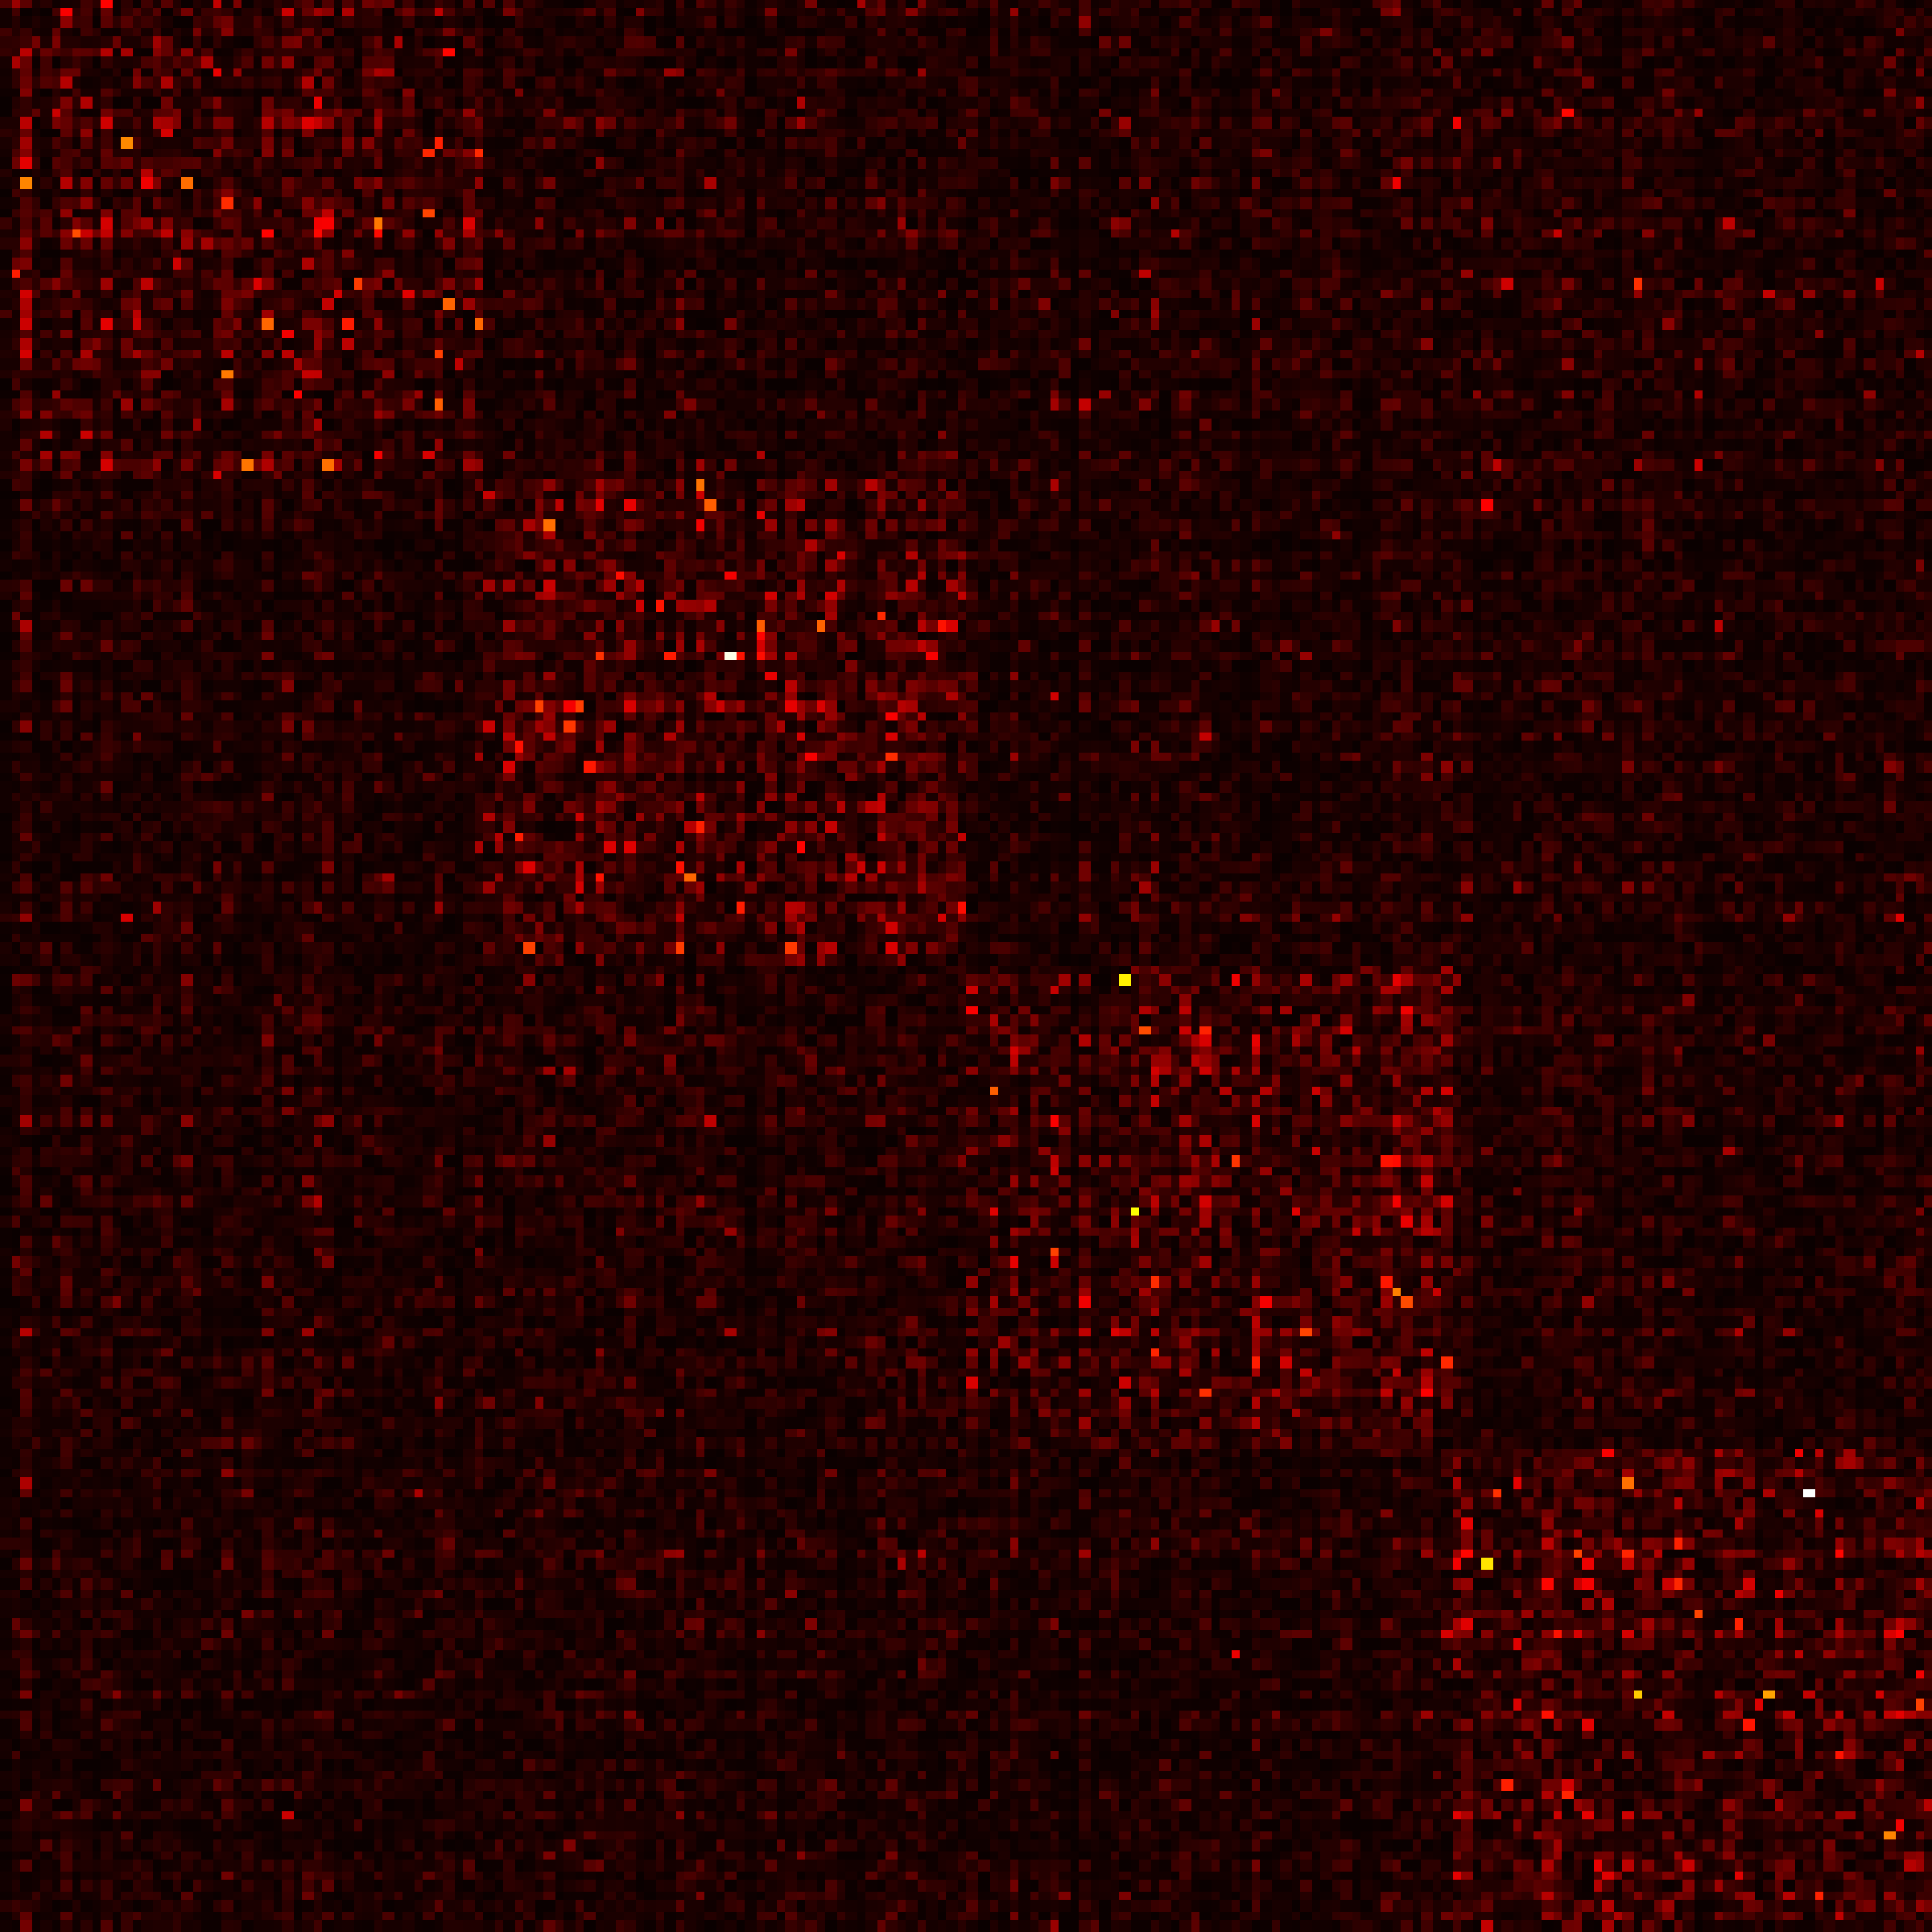
\includegraphics[width=\linewidth]{../Figs/Raster/msrc-cifar-nin-4pad-funnel8-convonly-conv8-corr}}
%    \caption{\textbf{Root-8:} 4 filter groups}
%    \label{fig:root8corr}
%\end{subfigure}
~
\begin{subfigure}[b]{0.31\linewidth}
\centering
    \covarlabels{\includegraphics[width=\linewidth]{../Figs/Raster/msrc-cifar-nin-4pad-funnel32-convonly-conv8-corr}}
    \caption{\textbf{Root-32:} $g=16$}
    \label{fig:root32corr}
\end{subfigure}
\caption{The block-diagonal sparsity learned by a root-module is visible in the correlation of filters on layers \texttt{conv3a} and \texttt{conv2c} in the NiN network.}
\label{fig:covar}
\end{figure}
%Figure~\ref{fig:covar} shows the inter-layer correlation between the adjacent filter layers \texttt{conv2c} and \texttt{conv3a} in the network architectures outlined in Table~\ref{table:ninconfig} as evaluated on the CIFAR test set. The block-diagonalization enforced by the filter group structure (as illustrated in Fig.~\ref{fig:groupconfig}) is visible, more so with larger number of filter groups. This shows that the network learns an organization of filters such that the sparsely distributed strong filter relations, visible in \ref{fig:normalcovartest} as brighter pixels, are grouped into a denser block-diagonal structure, leaving a visibly darker, low-correlated background. See \S\ref{interlayercovar} for more images, and an explanation of their derivation.
\end{frame}

%%%%%%%%%%%%%%%%5

\begin{frame}
\pgfplotstableread[col sep=comma]{../rootdata/resnet50ma.csv}\gdatatable
\pgfplotstableread[col sep=comma]{../rootdata/resnet50maconvonly.csv}\codatatable
\pgfplotsset{major grid style={dotted,red}}

\pgfplotstableset{
    create on use/singlecpu/.style={
        create col/expr={\thisrow{CPU Forward} / \thisrow{Batch Size}}},
}

\centering
\begin{tikzpicture}
\begin{axis}[
  width=\linewidth,
  height=0.45\linewidth,
  axis x line=bottom,
  ylabel=Top-5 Error,
  xlabel=Model Parameters (\# Floats),
  axis lines=left,
  enlarge x limits=0.05,
  %enlarge y limits=0.1,
  grid=major,
  %xmin=0,
  ytick={0.01,0.02,...,0.2},
  ymin=0.07,ymax=0.1,
  xticklabel style={
        /pgf/number format/fixed,
        /pgf/number format/precision=3
  },
  yticklabel={\pgfmathparse{\tick*100}\pgfmathprintnumber{\pgfmathresult}\%},style={
        /pgf/number format/fixed,
        /pgf/number format/precision=1
  },
  legend style={at={(0.98,0.98)}, anchor=north east, column sep=0.5em},
  legend columns=3,
]
\addplot[mark=*,mark options={fill=red},
   %nodes near coords,
   only marks,
   point meta=explicit symbolic,
] table[meta=Network,x=Param.,y expr={1 - \thisrow{Top-5 Acc.} },]{\gdatatable};
\addplot[mark=square*,mark options={fill=green},
   nodes near coords, nodes near coords align = {below}, only marks,
   every node near coord/.append style={inner sep=4pt},
   only marks,
   point meta=explicit symbolic,
] table[meta=Network,x=Param.,y expr={1 - \thisrow{Top-5 Acc.} },]{\codatatable};
\legend{ResNet 50, All Filters, Spatial Filters, LDE Half}
\end{axis}
\end{tikzpicture}

\pgfplotstableread[col sep=comma]{../rootdata/resnet50ma.csv}\gdatatable
\pgfplotstableread[col sep=comma]{../rootdata/resnet50maconvonly.csv}\codatatable
\pgfplotsset{major grid style={dotted,red}}

\centering
\begin{tikzpicture}
\begin{axis}[
  width=\linewidth,
  height=0.45\linewidth,
  axis x line=bottom,
  ylabel=Top-5 Error,
  xlabel=FLOPS (Multiply-Add),
  axis lines=left,
  enlarge x limits=0.05,
  %enlarge y limits=0.1,
  grid=major,
  %xmin=0,
  ytick={0.01,0.02,...,0.2},
  ymin=0.07,ymax=0.1,
  xticklabel style={
        /pgf/number format/fixed,
        /pgf/number format/precision=3
  },
  yticklabel={\pgfmathparse{\tick*100}\pgfmathprintnumber{\pgfmathresult}\%},style={
        /pgf/number format/fixed,
        /pgf/number format/precision=1
  },
  legend style={at={(0.98,0.98)}, anchor=north east, column sep=0.5em},
  legend columns=3,
]
\addplot[mark=*,mark options={fill=red},
   %nodes near coords,
   only marks,
   point meta=explicit symbolic,
] table[meta=Network,x=Multiply-Acc.,y expr={1 - \thisrow{Top-5 Acc.} },]{\gdatatable};
\addplot[mark=square*,mark options={fill=green},
   nodes near coords, nodes near coords align = {below}, only marks,
   every node near coord/.append style={inner sep=4pt},
   only marks,
   point meta=explicit symbolic,
] table[meta=Network,x=Multiply-Acc.,y expr={1 - \thisrow{Top-5 Acc.} },]{\codatatable};
\end{axis}
\end{tikzpicture}

\end{frame}

%%%%%%%%%%%%%%%%%%%%

\begin{frame}
\pgfplotstableread[col sep=comma]{../rootdata/resnet50ma.csv}\gdatatable
\pgfplotstableread[col sep=comma]{../rootdata/resnet50maconvonly.csv}\codatatable
\pgfplotsset{major grid style={dotted,red}}

\centering
\begin{tikzpicture}
\begin{axis}[
  width=\linewidth,
  height=0.45\linewidth,
  axis x line=bottom,
  ylabel=Top-5 Error,
  xlabel=GPU Forward (ms),
  axis lines=left,
  enlarge x limits=0.05,
  %enlarge y limits=0.1,
  grid=major,
  %xmin=0,
  ytick={0.01,0.02,...,0.2},
  ymin=0.07,ymax=0.1,
  xticklabel style={
        /pgf/number format/fixed,
        /pgf/number format/precision=3
  },
  yticklabel={\pgfmathparse{\tick*100}\pgfmathprintnumber{\pgfmathresult}\%},style={
        /pgf/number format/fixed,
        /pgf/number format/precision=1
  },
  legend style={at={(0.98,0.98)}, anchor=north east, column sep=0.5em},
  legend columns=3,
]
\addplot[mark=*,mark options={fill=red},
   %nodes near coords,
   only marks,
   point meta=explicit symbolic,
] table[meta=Network,
    x expr={\thisrow{GPU Forward} / \thisrow{Batch Size}},
    y expr={1 - \thisrow{Top-5 Acc.} }
]{\gdatatable};
\addplot[mark=square*,mark options={fill=green},
   nodes near coords, nodes near coords align = {below}, only marks,
   every node near coord/.append style={inner sep=4pt},
   only marks,
   point meta=explicit symbolic,
] table[meta=Network,
    x expr={\thisrow{GPU Forward} / \thisrow{Batch Size}},
    y expr={1 - \thisrow{Top-5 Acc.} },
]{\codatatable};
%\legend{ResNet 50, All Filters, Spatial Filters}
\end{axis}
\end{tikzpicture}

\pgfplotstableread[col sep=comma]{../rootdata/resnet50ma.csv}\gdatatable
\pgfplotstableread[col sep=comma]{../rootdata/resnet50maconvonly.csv}\codatatable
\pgfplotsset{major grid style={dotted,red}}

\centering
\begin{tikzpicture}
\begin{axis}[
  width=\linewidth,
  height=0.45\linewidth,
  axis x line=bottom,
  ylabel=Top-5 Error,
  xlabel=CPU Forward (ms),
  axis lines=left,
  enlarge x limits=0.05,
  %enlarge y limits=0.1,
  grid=major,
  %xmin=0,
  ytick={0.01,0.02,...,0.2},
  ymin=0.07,ymax=0.1,
  xticklabel style={
        /pgf/number format/fixed,
        /pgf/number format/precision=3
  },
  yticklabel={\pgfmathparse{\tick*100}\pgfmathprintnumber{\pgfmathresult}\%},style={
        /pgf/number format/fixed,
        /pgf/number format/precision=1
  },
  legend style={at={(0.98,0.98)}, anchor=north east, column sep=0.5em},
  legend columns=3,
]
\addplot[mark=*,mark options={fill=red},
   %nodes near coords,
   only marks,
   point meta=explicit symbolic,
] table[meta=Network,
    x expr={\thisrow{CPU Forward} / \thisrow{Batch Size}},
    y expr={1 - \thisrow{Top-5 Acc.} },
]{\gdatatable};
\addplot[mark=square*,mark options={fill=green},
   nodes near coords, nodes near coords align = {below}, only marks,
   every node near coord/.append style={inner sep=4pt},
   only marks,
   point meta=explicit symbolic,
] table[meta=Network,
    x expr={\thisrow{CPU Forward} / \thisrow{Batch Size}},
    y expr={1 - \thisrow{Top-5 Acc.} },
]{\codatatable};
%\legend{ResNet 50, All Filters, Spatial Filters}
\end{axis}
\end{tikzpicture}

\end{frame}

%%%%%%%%%%%%%%%%%%%%

\begin{frame}{Imagenet Results}

%We propose a new method for creating computationally efficient and compact convolutional neural networks (CNNs) using a novel sparse connection structure that resembles a tree root. This allows a significant reduction in computational cost and number of parameters compared to state-of-the-art deep CNNs, without compromising accuracy, by exploiting the sparsity of inter-layer filter dependencies. We validate our approach by using it to train more efficient variants of state-of-the-art CNN architectures, evaluated on the CIFAR10 and ILSVRC datasets. Our results show similar or higher accuracy than the baseline architectures with much less computation, as measured by CPU and GPU timings. For example, for ResNet 50, our model has 40% fewer parameters, 45% fewer floating point operations, and is 31% (12%) faster on a CPU (GPU). For the deeper ResNet 200 our model has 25% fewer floating point operations and 44% fewer parameters, while maintaining state-of-the-art accuracy. For GoogLeNet, our model has 7% fewer parameters and is 21% (16%) faster on a CPU (GPU).
Networks with root modules have similar or higher accuracy than the baseline architectures with much less computation.
\begin{itemize}
    \item ResNet 50\footnote{Caffe Re-implementation}: \textbf{40\%} smaller, \textbf{45\%} fewer FLOPS%, and is 31\% (12\%) faster on a CPU (GPU).
    \item ResNet 200\footnote{Based on Facebook Torch Model}: \textbf{44\%} smaller, \textbf{25\%} fewer FLOPS
    \item GoogLeNet: \textbf{7\%} smaller, \textbf{44\%} fewer FLOPS%, and is 21\% (16\%) faster on a CPU (GPU)
\end{itemize}
\vfill
But when you also \textbf{increase the number of filters}\ldots
\end{frame}

%%%%%%%%%%%%%%%%%%%%

\usebackgroundtemplate{
\tikz[overlay,remember picture] \node[opacity=0.5, at=(current page.center), yshift=-1cm] {
\centering
   \setlength{\fboxsep}{0pt}\setlength\fboxrule{0.5pt}\fbox{
   \includegraphics[width=0.9\paperwidth,page=1]{resnext.pdf}
   }
   };
}

\begin{frame}
\vfill
\centering
\colorbox{white}{
\setlength{\fboxsep}{0pt}\fbox{
\begin{minipage}{0.6\paperwidth}
   \includegraphics[width=0.6\paperwidth,page=1]{resnext-filterconfig.pdf}
   
   \begin{quote}
   \footnotesize
   ``Moreover, increasing cardinality is more effective than going deeper or wider when we increase the capacity.''
   \end{quote}
\end{minipage}
}
}
\end{frame}

\usebackgroundtemplate{}

%%%%%%%%%%%%%%%%%%%%
\section{Summary/Future Work}

%%%%%%%%%%%%%%%%%%%%
\begin{frame}{Summary}

  % Keep the summary *very short*.
  \begin{itemize}
	%\item Separable filter model show surprisingly high accuracy on what are considered challenging problems -- approx.\ 88\% top-5 accuracy on ILSVRC.
	\item Using structural priors:
	\begin{itemize}
    	\item Models are \textbf{less computationally complex}
	    \item They also use \textbf{less parameters}
	    \item They significantly help generalization in \textbf{deeper networks}
        \item They significantly help generalization with \textbf{larger datasets}
	\end{itemize}
	\item Are amenable to \textbf{model parallelization} (as with original AlexNet), for better parallelism across gpus/nodes
	%\item The restriction on what filter responses may be combined is an effective form of regularization, and helps prevent over-fitting.
  \end{itemize}
\end{frame}

%%%%%%%%%%%%%%%%%%%%
\begin{frame}{Future Work: Research}
    \begin{itemize}
        \item We don't always have enough knowledge of the domain to propose good structural priors
        \item Our results (and follow up work) do show however that current methods of training/regularization seem to have limited effectiveness in DNNs learning such priors themselves
        \item How can we otherwise learn structural priors?
    \end{itemize}
\end{frame}

\begin{frame}{Future Work: Applications}
    Both of these methods apply to most deep learning applications:
    \begin{itemize}
        \item Smaller model state -- easier storage and synchronization
        \item Faster training and test of models behind ML cloud services
        \item Embedded devices/Tensor processing units
    \end{itemize}
    And more specific to each method
    \begin{itemize}
        \item Low-rank filters
        \begin{itemize}
            \item Even larger impact for volumetric imagery (Microsoft Radiomics)
        \end{itemize}
        \item Root Modules
        \begin{itemize}
            \item Model parallelization (Azure/Amazon Cloud)
        \end{itemize}
    \end{itemize}
\end{frame}


%%%%%%%%%%%%%%%%%%%%

  \usebackgroundtemplate{
  \tikz[overlay,remember picture] \node[opacity=0.2, at=(current page.center)] {
  \includegraphics[height=\paperheight,width=\paperwidth]{background}};
  }

  \begin{frame}
  \vfill
  \centering
  %\begin{beamercolorbox}[sep=8pt,center,shadow=true,rounded=true]{title}
    \usebeamerfont{title}Extra Slides\par%
  %\end{beamercolorbox}
  \vfill
  \end{frame}
  
  \usebackgroundtemplate{}

%%%%%%%%%%%%%%%%%%%%

\begin{frame}{AlexNet Complexity}
\begin{figure}[tbp]
\centering
\tikzstyle{every node}=[font=\tiny]
\pgfplotstableread[col sep=comma]{alexnetma.csv}\datatable
\begin{tikzpicture}
\begin{axis}[
    axis x line=bottom,
    axis y line=left,
    ybar=0pt,
    bar width=1em,
    width=0.9\linewidth,
    height=0.33\linewidth,
    enlarge x limits=0.1,
    ylabel=FLOPS,
    y label style={at={(axis description cs:0.09,.5)},anchor=south},
    y tick label style={
        /pgf/number format/.cd,
            fixed,
            fixed zerofill,
            precision=1,
        /tikz/.cd
    },
    ymin=0,
    xmajorticks=false,
    legend style={at={(0.5,1.2)},
    draw=none, anchor=north,legend columns=-1},
    area legend,
]
\addplot[ybar, draw=none, fill=red!40] table [x expr=\coordindex,y=ma]{\datatable};
\end{axis}
\end{tikzpicture}
~
\begin{tikzpicture}
\begin{axis}[
    axis x line=bottom,
    axis y line=left,
    ybar=0pt,
    bar width=1em,
    width=0.9\linewidth,
    height=0.33\linewidth,
    enlarge x limits=0.1,
    ylabel=Parameters,
    y label style={at={(axis description cs:0.09,.5)},anchor=south},
    y tick label style={
        /pgf/number format/.cd,
            fixed,
            fixed zerofill,
            precision=1,
        /tikz/.cd
    },
    ymin=0,
    xticklabels from table={\datatable}{layer},
    xticklabel style = {rotate = 90, xshift = -0.8ex, anchor = mid east, font=\tiny},
    xtick=data,
]
\addplot[ybar, draw=none, fill=red!40] table [x expr=\coordindex,y=param]{\datatable};
\end{axis}
\end{tikzpicture}
\end{figure}
\end{frame}
%%%%%%%%%%%%%%%%%%%%

\begin{frame}{Typical Convolutional Layer}
\begin{figure}
   \includegraphics[width=0.9\textwidth, page=1]{../Figs/PDF/groupfig}
%   \caption{A full rank convolutional layer.}
\end{figure}
    Best example of this idea is a CNN!
    \begin{itemize}
        \item Shared parameters: filter learned for one part of the image should apply to the whole image.
        \item Filters: natural images are highly correlated locally
    \end{itemize}
    %\item A fully-connected network could theoretically learn the same thing, but in practice it never will.

    \note[item]{We show here a typical convolutional layer.}
    \note[item]{Yellow blocks are filters.}
    \note[item]{Grey blocks are images or feature maps.}
\end{frame}
%%%%%%%%%%%%%%%%%%%%
\begin{frame}{Vanishing/Exploding Gradients}{}
\vspace{-2em}
\begin{figure}
%\begin{tikzpicture}
    %\node[inner sep=0pt] (1) at (0,0)
    %{
    \includegraphics[width=0.2\textwidth, page=1, bb = 0 0 440 600, clip=true]{../Figs/PDF/sparsification}
    \includegraphics[width=0.2\textwidth, page=1, bb = 0 0 440 600, clip=true]{../Figs/PDF/sparsification}
    \includegraphics[width=0.2\textwidth, page=1, bb = 0 0 440 600, clip=true]{../Figs/PDF/sparsification}
    %};
    %\node[inner sep=0pt] (2) at (5,0)
    %{
    $\cdots$
    \includegraphics[width=0.2\textwidth, page=1, bb = 0 0 400 600, clip=true]{../Figs/PDF/sparsification}
    %};
    %\node at ($(1.south east)!.5!(2.south west)$) {\ldots};
%\end{tikzpicture}
\end{figure}

\begin{itemize}
    \item Incorrect initialization scales the forward signal by $\beta$.
    \item After $L$ layers, this becomes a scaling of $\beta^L$.
    \item For \alert{$\beta > 1$}, signal $\rightarrow\infty$, training \alert{diverges}.
    \item For \alert{$\beta < 1$}, signal $\rightarrow 0$, training \alert{stalls}.
    \item Want $\beta\approx 1$ in all layers to prevent this.
\end{itemize}
\note[item]{at the end of this layer, have a softmax!}
\note[item]{$\sigma(\mathbf{z})_j = \frac{e^{z_j}}{\sum_{k=1}^K e^{z_k}}$.}
\end{frame}

%%%%%%%%%%%%%%%%%%%%
\begin{frame}{Convolutional Layer - Initialization}
\begin{figure}
\includegraphics[width=0.7\textwidth, page=1]{../Figs/PDF/sparsification}
\end{figure}
For a sigmoid non-linearity\footcite{glorot2010understanding}:
\begin{eqnarray*}
\sigma &=& \sqrt{\frac{1}{n^{\textrm{ out}}}} = \sqrt{\frac{2}{w^{[i]} h^{[i]} d^{[i]}}}.
\end{eqnarray*}
For a ReLU non-linearity\footcite{He2015}:
\begin{equation*}
\sigma = \sqrt{\frac{2}{n^{\textrm{ out}}}}.
\end{equation*}
\end{frame}

%%%%%%%%%%%%%%%%%%%%

\begin{frame}{Convolution is Expensive}{Can we use Separable Filters?}
\begin{itemize}
    \item In image processing, we can often use separable filters instead.
    \begin{itemize}
        \item Factorizes a $k\times k$ filter into $1\times k$ and $k \times 1$ smaller filters.
        \item Only works if we can factorize a matrix into such an outer product $\Rightarrow$ rank-1 matrix    \item \eg $\begin{bmatrix} 1 \\ 2 \\ 1\end{bmatrix} \begin{bmatrix} -1 & 0 & 1\end{bmatrix}  = \begin{bmatrix} -1 & 0 & 1 \\ -2 & 0 & 2 \\ -1 & 0 & 1\end{bmatrix}$.
    \end{itemize}
    
    % The following outlook is optional.
    \vskip0pt plus.5fill
    \item Much faster - $\mathcal{O}(k+k)$ \vs $\mathcal{O}(k^2)$.
    \note[item]{We can do this because convolution is associative, \ie $f*(v*h) = (f*v)*h$.}
\end{itemize}
\end{frame}

%%%%%%%%%%%%%%%%%%%%

\begin{frame}{Separable Layer}
\vspace{-1em}
\begin{itemize}
    \item Use sequential filters of differing orientation\footcite{mamalet2012simplifying,journals/corr/JaderbergVZ14}.
\end{itemize}
\begin{figure}
    \begin{tikzpicture}
        \node at (0, 4.2) (n1) {
            \includegraphics[width=0.4\textwidth, page=1]{../Figs/PDF/sparsification}
        };
        \node at (0, 1) (t1) {
            \includegraphics[width=0.9\textwidth, page=2]{../Figs/PDF/sparsification}
        };
        \path[->]<1-> (n1) edge (t1);
    \end{tikzpicture}
\end{figure}

\end{frame}
%%%%%%%%%%%%%%%%%%%%

\begin{frame}{Separable Layer -- Issues}
\begin{figure}
\includegraphics[width=\textwidth, page=2]{../Figs/PDF/sparsification}
%   \caption{Sequential separable filters.}
%   \label{fig:separableseq}
\end{figure}
\begin{itemize}
    \item Order of filter orientations gives different results (!).
    \note[item]{Vertical first was more accurate\footcite{mamalet2012simplifying}}
    \note[item]{Second orientation has $64\times$ the param, overfits differently?}
    \item Complexity of each filter:
    \begin{itemize}
        \item before: filter is $\mathcal{O}(d \times [h\times w \times c])$.
        \item after: $\mathcal{O}(d\times [h\times \mathbf{m}] + \mathbf{m} [w \times c])$,
    \end{itemize}
    \item However, in practice was not trainable for large networks.
    \item New initialization proposed allows us to train this.
    \note[item]{Get vanishing/exploding gradients if we tried to train these networks.}
    \note[item]{in most CNNs, $d \geq m \gg c$, so still not that cheap.}
    \note[item]{Second orientation has $64\times$ the param, so much more expensive that you'd think.}
    \note[item]{Still has compute savings.}
\end{itemize}
\end{frame}

%%%%%%%%%%%%%%%%%%%%
\pgfplotstableread[col sep=comma]{../lrdata/bigpicture.csv}\datatable
\pgfplotstableread[col sep=comma]{../lrdata/bigpicture_ours.csv}\datatableours
\pgfplotstableread[col sep=comma]{../lrdata/bigpicture_aug.csv}\datatableaug
\pgfplotsset{major grid style={dotted,red}}
\pgfplotsset{minor grid style={dotted,red}}

\begin{frame}{State-of-the-Art Models}%{The Cost of Increasing Accuracy}
\resizebox {\textwidth} {!} {
\begin{tikzpicture}
\begin{axis}[
  width=1.2\textwidth,
  height=1.1\textheight,
  axis x line=bottom,
  ylabel=Top-5 Error,
  xlabel=$\log_{10}$(Multiply-Accumulate Operations),
  axis lines=left,
  enlarge x limits=0.05,
  enlarge y limits=0.05,
  grid=both,
  ytick={0.00,0.02,...,0.22},
  xmode=log, 
  %ymin=0,ymax=0.2,
  %xmin=10e8,xmax=10e10,
  yticklabel={\pgfmathparse{\tick*100}\pgfmathprintnumber{\pgfmathresult}\%},style={
        /pgf/number format/fixed,
        /pgf/number format/precision=1
  },
  legend style={at={(0.01,0.01)},anchor=south west},
]
\addplot[mark=*,mark options={fill=blue},nodes near coords,only marks,
   point meta=explicit symbolic,
   every node near coord/.append style={xshift=0.01em, anchor=west, font=\tiny},
] table[meta=Network,x=Multiply-Acc.,y expr={1 - \thisrow{Top-5 Acc.} }]{\datatable};
\addplot[mark=square*,mark options={fill=red},nodes near coords,only marks,
   point meta=explicit symbolic,
   every node near coord/.append style={xshift=0.01em, anchor=west, font=\tiny},
] table[meta=Network,x=Test Multiply-Acc.,y expr={1 - \thisrow{Top-5 Acc.} }]{\datatableaug};
\addplot[mark=*,mark options={fill=green!70!black},nodes near coords,only marks,
   point meta=explicit symbolic,
   every node near coord/.append style={xshift=0.01em, anchor=west, font=\tiny},
] table[meta=Network,x=Multiply-Acc.,y expr={1 - \thisrow{Top-5 Acc.} }]{\datatableours};
\legend{Crop \& Mirror Aug., Extra Augmentation, Our Results}
\end{axis}
\end{tikzpicture}
}
\end{frame}

%%%%%%%%%%%%%%%%%%%%

\begin{frame}{}
\begin{figure}
\centering
\pgfplotstableread[col sep=comma]{../lrdata/bigpicture.csv}\datatable
\pgfplotstableread[col sep=comma]{../lrdata/bigpicture_ours.csv}\datatableours
\pgfplotstableread[col sep=comma]{../lrdata/bigpicture_aug.csv}\datatableaug
\pgfplotsset{major grid style={dotted,red}}
\pgfplotsset{minor grid style={dotted,red}}

\resizebox {\textwidth} {!} {
\begin{tikzpicture}
\begin{axis}[
  width=1.2\textwidth,
  height=1.1\textheight,
  axis x line=bottom,
  ylabel=Top-5 Error,
  xlabel=$\log_{10}$(Number of Parameters),
  axis lines=left,
  enlarge y limits=0.05,
  grid=both,
  ytick={0.01,0.02,...,0.2},
  xmode=log,
  xmin=10e5,xmax=10e8,
  yticklabel={\pgfmathparse{\tick*100}\pgfmathprintnumber{\pgfmathresult}\%},style={
        /pgf/number format/fixed,
        /pgf/number format/precision=1
  },
  legend style={at={(0.01,0.01)},anchor=south west},
]
\addplot[mark=*,mark options={fill=blue},
   nodes near coords,
   only marks,
   point meta=explicit symbolic,
   every node near coord/.append style={xshift=0.01em, anchor=west, font=\tiny},
] table[meta=Network,x=Param.,y expr={1 - \thisrow{Top-5 Acc.} }]{\datatable};
\addplot[mark=square*,mark options={fill=red},
   nodes near coords,
   only marks,
   point meta=explicit symbolic,
   every node near coord/.append style={xshift=0.01em, anchor=west, font=\tiny},
   every node near coord/.append style={font=\tiny},
] table[meta=Network,x=Param.,y expr={1 - \thisrow{Top-5 Acc.} }]{\datatableaug};
\addplot[mark=*,mark options={fill=green!70!black},
   nodes near coords,
   only marks,
   point meta=explicit symbolic,
   every node near coord/.append style={xshift=0.01em, anchor=west, font=\tiny},
] table[meta=Network,x=Param.,y expr={1 - \thisrow{Top-5 Acc.} }]{\datatableours};
\legend{Crop \& Mirror Aug., Extra Augmentation, Our Results}
\end{axis}
\end{tikzpicture}
}
\end{figure}
\end{frame}
%%%%%%%%%%%%%%%%%%%%
\renewcommand{\covarlabels}[5]{%
\begin{tikzpicture}[anchor=south west]
    \tikzstyle{every node}=[font=\tiny]
    \node [inner sep=0pt] (c)
    {
        #5
    };
    \ifx\covarwidth\undefined
    \newlength{\covarwidth}
    \newlength{\covarheight}
    \fi
    \settowidth{\covarwidth}{#5}
    \settoheight{\covarheight}{#5}
    \path[use as bounding box] (c.south west) rectangle (c.north east);
    %\node [anchor=south west, xshift=-0.5em, yshift=-0.5em, rotate=45] at (c.north west) {\footnotesize 0};
    %\node [anchor=south east, xshift=\covarwidth, yshift=-0.2em] at (c.north west) {\footnotesize #4};
    %\node [anchor=south west, xshift=0.25em, yshift=-1.05\covarheight, rotate=90] at (c.north west) {\footnotesize #2};
    \node [anchor=south, xshift=0.5\covarwidth] at (c.north west) {\tiny\texttt{#3}};
    %\node [anchor=south, xshift=0.2em, yshift=-0.5\covarheight, rotate=90] at (c.north west) {\footnotesize \texttt{#1}};
\end{tikzpicture}%
}

\begin{frame}[fragile]{Intra-layer Filter Correlation}
\centering
\tiny
%    \covarlabels{conv1a}{192}{conv1a}{192}{\includegraphics[width=0.1\textwidth]{../Figs/Raster/nin/corrcoef_conv0.png}}
%~
%    \covarlabels{conv1b}{160}{conv1b}{160}{\includegraphics[width=0.1\textwidth]{../Figs/Raster/nin/corrcoef_conv1.png}}
%~
    \covarlabels{conv1c}{96}{conv1c}{96}{\includegraphics[width=0.15\textwidth]{../Figs/Raster/nin/corrcoef_conv2.png}}
    \covarlabels{conv2a}{192}{conv2a}{192}{\includegraphics[width=0.15\textwidth]{../Figs/Raster/nin/corrcoef_conv4.png}}
    \covarlabels{conv2b}{192}{conv2b}{192}{\includegraphics[width=0.15\textwidth]{../Figs/Raster/nin/corrcoef_conv5.png}}
    \covarlabels{conv2c}{192}{conv2c}{192}{\includegraphics[width=0.15\textwidth]{../Figs/Raster/nin/corrcoef_conv6.png}}
    \covarlabels{conv3a}{192}{conv3a}{192}{\includegraphics[width=0.15\textwidth]{../Figs/Raster/nin/corrcoef_conv8.png}}
    \covarlabels{conv3b}{192}{conv3b}{192}{\includegraphics[width=0.15\textwidth]{../Figs/Raster/nin/corrcoef_conv9.png}}\\
\textbf{Network-in-Network.}\\
%    \covarlabels{conv1a}{192}{conv1a}{192}{\includegraphics[width=0.11\textwidth]{../Figs/Raster/ninroot4/corrcoef_conv0.png}}
%~
%    \covarlabels{conv1b}{160}{conv1b}{160}{\includegraphics[width=0.11\textwidth]{../Figs/Raster/ninroot4/corrcoef_conv1.png}}
%~
    \includegraphics[width=0.15\textwidth]{../Figs/Raster/ninroot4/corrcoef_conv2.png}
~
    \includegraphics[width=0.15\textwidth]{../Figs/Raster/ninroot4/corrcoef_conv4.png}
~
    \includegraphics[width=0.15\textwidth]{../Figs/Raster/ninroot4/corrcoef_conv5.png}
~
    \includegraphics[width=0.15\textwidth]{../Figs/Raster/ninroot4/corrcoef_conv6.png}
~
    \includegraphics[width=0.15\textwidth]{../Figs/Raster/ninroot4/corrcoef_conv8.png}
~
    \includegraphics[width=0.15\textwidth]{../Figs/Raster/ninroot4/corrcoef_conv9.png}\\
\textbf{Root-4.}\\
%    \covarlabels{conv1a}{192}{conv1a}{192}{\includegraphics[width=0.15\textwidth]{../Figs/Raster/ninroot8/corrcoef_conv0.png}}
%~
%    \covarlabels{conv1b}{160}{conv1b}{160}{\includegraphics[width=0.15\textwidth]{../Figs/Raster/ninroot8/corrcoef_conv1.png}}
%~
    \includegraphics[width=0.15\textwidth]{../Figs/Raster/ninroot8/corrcoef_conv2.png}
~
    \includegraphics[width=0.15\textwidth]{../Figs/Raster/ninroot8/corrcoef_conv4.png}
~
    \includegraphics[width=0.15\textwidth]{../Figs/Raster/ninroot8/corrcoef_conv5.png}
~
    \includegraphics[width=0.15\textwidth]{../Figs/Raster/ninroot8/corrcoef_conv6.png}
~
    \includegraphics[width=0.15\textwidth]{../Figs/Raster/ninroot8/corrcoef_conv8.png}
~
    \includegraphics[width=0.15\textwidth]{../Figs/Raster/ninroot8/corrcoef_conv9.png}\\
\textbf{Root-8.}\\
%    \covarlabels{conv1a}{192}{conv1a}{192}{\includegraphics[width=0.15\textwidth]{../Figs/Raster/ninroot32/corrcoef_conv0.png}}
%~
%    \covarlabels{conv1b}{160}{conv1b}{160}{\includegraphics[width=0.15\textwidth]{../Figs/Raster/ninroot32/corrcoef_conv1.png}}
%~
    \includegraphics[width=0.15\textwidth]{../Figs/Raster/ninroot32/corrcoef_conv2.png}
~
    \includegraphics[width=0.15\textwidth]{../Figs/Raster/ninroot32/corrcoef_conv4.png}
~
    \includegraphics[width=0.15\textwidth]{../Figs/Raster/ninroot32/corrcoef_conv5.png}
~
    \includegraphics[width=0.15\textwidth]{../Figs/Raster/ninroot32/corrcoef_conv6.png}
~
    \includegraphics[width=0.15\textwidth]{../Figs/Raster/ninroot32/corrcoef_conv8.png}
~
    \includegraphics[width=0.15\textwidth]{../Figs/Raster/ninroot32/corrcoef_conv9.png}\\
\textbf{Root-32.}\\
\includegraphics[width=0.4\linewidth]{../Figs/PDF/colorbar}
\end{frame}

%%%%%%%%%%%%%%%%%%%%

\renewcommand{\covarlabels}[5]{%
\begin{tikzpicture}[anchor=south west]
    \node [inner sep=0pt] (c)
    {
        #5
    };
    \ifx\covarwidth\undefined
    \newlength{\covarwidth}
    \newlength{\covarheight}
    \fi
    \settowidth{\covarwidth}{#5}
    \settoheight{\covarheight}{#5}
    \path[use as bounding box] (c.south west) rectangle (c.north east);
    \node [anchor=south west, xshift=-0.5em, yshift=-0.5em, rotate=45] at (c.north west) {\footnotesize 0};
    \node [anchor=south east, xshift=\covarwidth, yshift=-0.2em] at (c.north west) {\footnotesize #4};
    \node [anchor=south west, xshift=0.25em, yshift=-1.05\covarheight, rotate=90] at (c.north west) {\footnotesize #2};
    \node [anchor=south, xshift=0.5\covarwidth] at (c.north west) {\footnotesize\texttt{#3}};
    \node [anchor=south, xshift=0.2em, yshift=-0.5\covarheight, rotate=90] at (c.north west) {\footnotesize \texttt{#1}};
\end{tikzpicture}%
}

\begin{frame}{Whitening for Covariance Analysis}

\begin{figure}[tbp]
\centering
\begin{subfigure}[b]{0.45\linewidth}
\centering
    \covarlabels{conv2c}{192}{conv3a}{192}{\includegraphics[width=\linewidth]{../Figs/Raster/ninroot32/layercovar_conv8.png}}
    \caption{Non-whitened responses}
    \label{fig:notwhitened}
\end{subfigure}
\hfill
\begin{subfigure}[b]{0.45\linewidth}
\centering
    \covarlabels{conv2c}{192}{conv3a}{192}{\includegraphics[width=\linewidth]{../Figs/Raster/ninroot32/layercovarwhite_conv8.png}}
    \caption{Whitened responses}
    \label{fig:whitened}
\end{subfigure}
\caption{Covariance between layers is conflated with the inherent covariances within $X_1$ and $X_2$ from the data. We can more clearly show the covariance between layers by first whitening (using ZCA~\citep{CIFAR10}) the samples in $X_1$ and $X_2$.}
\label{fig:whitevsnot}
\end{figure}
\end{frame}

%%%%%%%%%%%%%%%%%%%%%%%

\subsection{Collaborative Research}
\begin{frame}{Collaborative Research @ MSR}
\begin{itemize}
    \item \textbf{Medical Computer Vision}
    \begin{itemize}
        \item Segmentation of brain tumor tissues with convolutional neural networks.\\{\footnotesize D.\ Zikic, Y.\ Ioannou, M.\ Brown, A.\ Criminisi.}\\%\\\textit{MICCAI-BRATS 2014}}
        \item Using CNNs for Malaria Diagnosis.\\{\footnotesize Intellectual Ventures/Gates Foundation}
    \end{itemize}
    \item \textbf{Adversarial Examples}\\Measuring Neural Net Robustness with Constraints.\\{\footnotesize O.\ Bastani, Y.\ Ioannou, L.\ Lampropoulos, D.\ Vytiniotis, A.\ Nori, A.\ Criminisi.}%\\\textit{NIPS 2016}}
    \item \textbf{Neural Network Design}\\Refining Architectures of Deep Convolutional Neural Networks.\\{\footnotesize 
S.\ Shankar, D.\ Robertson, Y.\ Ioannou, A.\ Criminisi, R.\ Cipolla.}%\\\textit{CVPR 2016}}
\end{itemize}
\end{frame}


\usebackgroundtemplate{%             declare it
\tikz[overlay,remember picture] \node[opacity=0.7, at=(current page.center), yshift=-8cm] {
   \setlength{\fboxsep}{0pt}\fbox{
   \includegraphics[width=0.9\paperwidth,page=2]{darkobrats.pdf}
   }
   };
}

\begin{frame}{Collaborative Research @ MSR}
\textbf{Segmentation of brain tumor tissues with convolutional neural networks}\\{\footnotesize D.\ Zikic, Y.\ Ioannou, M.\ Brown, A.\ Criminisi.\\\textit{MICCAI-BRATS 2014}}
\begin{itemize}
    \item One of the first papers using deep learning for volumetric/medical imagery
    %\item Biggest challenge for training was the class-imbalanced training data
\end{itemize}
\vfill
\end{frame}

\usebackgroundtemplate{}

\begin{frame}{Collaborative Research @ MSR}
\textbf{Using CNNs for Malaria Diagnosis}\\{\footnotesize Intellectual Ventures/Gates Foundation}
\begin{itemize}
    \item Design and train CNN for the classification of malaria parasites in blood smears.
\end{itemize}
\vfill
\includegraphics[width=0.45\linewidth]{malarianegative}\hfill\includegraphics[width=0.45\linewidth]{malariapositive}
\end{frame}


\usebackgroundtemplate{%             declare it
\tikz[overlay,remember picture] \node[opacity=0.7, at=(current page.center), yshift=-7cm] {
   \setlength{\fboxsep}{0pt}\fbox{
   \includegraphics[width=0.9\paperwidth,page=1]{osbertnips.pdf}
   }
   };
}

\begin{frame}{Collaborative Research @ MSR}
\textbf{Measuring Neural Net Robustness with Constraints}\\{\footnotesize O.\ Bastani, Y.\ Ioannou, L.\ Lampropoulos, D.\ Vytiniotis, A.\ Nori, A.\ Criminisi.\\\textit{NIPS 2016}}
\begin{itemize}
    %\item Showed that contemporary methods of finding adversarial examples were limited in their coverage
    \item Found that not all adversarial images can be used to improve network robustness
\end{itemize}
\end{frame}


\usebackgroundtemplate{%             declare it
\tikz[overlay,remember picture] \node[opacity=0.7, at=(current page.center), yshift=-8cm] {
   \setlength{\fboxsep}{0pt}\fbox{
   \includegraphics[width=0.9\paperwidth,page=1]{sukritcvpr.pdf}
   }
   };
}

\begin{frame}{Collaborative Research @ MSR}
\textbf{Refining Architectures of Deep Convolutional Neural Networks}\\{\footnotesize S.\ Shankar, D.\ Robertson, Y.\ Ioannou, A.\ Criminisi, R.\ Cipolla.\\\textit{CVPR 2016}}
\begin{itemize}
    \item A method for adapting network architectures optimized for one dataset to another
    %\item Attempts to answer the common problem of adapting contemporary research to real-world problems
\end{itemize}
\end{frame}

\usebackgroundtemplate{}


\end{document}


